% =====================================================================
%  Tesis de Cipriano Ezequiel Pereira López — versión corregida (v2)
%  Compilar: latexmk -pdf main.tex   (pdflatex + biber)
% =====================================================================
\documentclass[12pt,letterpaper,oneside,openany]{report}

% ---------- Idioma y codificación ----------
\usepackage[utf8]{inputenc}
% Vocales nasales del guaraní que inputenc no trae definidas (Ñemombyky)
\DeclareUnicodeCharacter{1EBD}{\~e}
\DeclareUnicodeCharacter{1EF9}{\~y}
\usepackage[T1]{fontenc}
\usepackage{lmodern}
\usepackage[english,spanish,es-tabla,es-lcroman,es-nodecimaldot,es-noshorthands]{babel}
\usepackage{csquotes}

% ---------- Página ----------
% Hoja carta y márgenes de 2,54 cm, como el formato de referencia (APA 7).
% El margen superior de 3,81 cm deja lugar al membrete, que empieza a 0,5 cm del borde.
\usepackage[top=3.81cm,bottom=2.54cm,left=2.54cm,right=2.54cm,
            headheight=3.0cm,headsep=0.35cm,footskip=1.2cm]{geometry}
% Interlineado doble en todo el documento, como el formato de referencia (APA 7).
% Tablas, rótulos y notas al pie van a espacio simple (setspace lo hace en los
% flotantes y las notas); los listados y las tablas largas, más abajo.
\usepackage{setspace}
\doublespacing
\setlength{\parindent}{1.25cm}
\setlength{\parskip}{0pt}
\setlength{\emergencystretch}{2em}
\usepackage{ragged2e}
\usepackage{emptypage}
\usepackage{lastpage}

% ---------- Matemática ----------
\usepackage{amsmath,amssymb,bm}
\usepackage{etoolbox}
\usepackage{siunitx}
\sisetup{output-decimal-marker={,},group-separator={\,},per-mode=symbol}
% Las filas de las matrices usan el interlineado simple aunque el texto vaya a doble
\makeatletter
\newcommand{\filasimple}{\@tempdima=\f@baselineskip\relax
  \setbox\strutbox\hbox{\vrule\@height.7\@tempdima\@depth.3\@tempdima\@width\z@}}
\makeatother
\AtBeginEnvironment{bmatrix}{\filasimple}
\newcommand{\Aprime}{A$'$}
\newcommand{\IL}{I_L}

% ---------- Numeración e índice hasta subsubsecciones (marco referencial) ----------
\setcounter{secnumdepth}{3}
\setcounter{tocdepth}{3}

% ---------- Numeración continua de figuras, tablas y ecuaciones (APA) ----------
% Figura 1, Tabla 1, (1) en todo el cuerpo; en los anexos llevan la letra del anexo
\counterwithout{figure}{chapter}
\counterwithout{table}{chapter}
\counterwithout{equation}{chapter}

% ---------- Títulos ----------
% Capítulos (y títulos sin número: índices, referencias, anexos) centrados en
% negrita; tercer y cuarto nivel (1.2.1 y 1.2.1.1) en negrita cursiva, como en APA
\makeatletter
\renewcommand{\@makechapterhead}[1]{%
  \vspace*{20\p@}%
  {\centering\normalfont\setstretch{1}%
   \ifnum\c@secnumdepth>\m@ne
     {\Huge\bfseries\@chapapp\space\thechapter\par}\nobreak
     \vskip 20\p@
   \fi
   \interlinepenalty\@M
   {\LARGE\bfseries #1\par}\nobreak
   \vskip 40\p@}}
\renewcommand{\@makeschapterhead}[1]{%
  \vspace*{20\p@}%
  {\centering\normalfont\setstretch{1}%
   \interlinepenalty\@M
   {\LARGE\bfseries #1\par}\nobreak
   \vskip 40\p@}}
\renewcommand{\subsection}{\@startsection{subsection}{2}{\z@}%
  {-3.25ex\@plus -1ex \@minus -.2ex}{1.5ex \@plus .2ex}%
  {\normalfont\large\bfseries\itshape}}
\renewcommand{\subsubsection}{\@startsection{subsubsection}{3}{\z@}%
  {-3.25ex\@plus -1ex \@minus -.2ex}{1.5ex \@plus .2ex}%
  {\normalfont\normalsize\bfseries\itshape}}
\makeatother

% ---------- Figuras y tablas ----------
\usepackage{graphicx}
\graphicspath{{figuras/}{figuras/originales/}}
\usepackage{booktabs,longtable,array,multirow,makecell,tabularx}
\usepackage{pdflscape}
\usepackage{caption}
% Rótulos APA: número en negrita y, en la línea siguiente, el título en cursiva
\captionsetup{labelfont=bf,textfont=it,labelsep=newline,
              justification=raggedright,singlelinecheck=false}
\usepackage{float}
\usepackage{tikz}
\usetikzlibrary{arrows.meta,positioning,shapes.geometric,calc,fit}
\usepackage{xcolor}
\definecolor{metA}{HTML}{C0392B}
\definecolor{metAp}{HTML}{E67E22}
\definecolor{metB}{HTML}{2E86C1}
\definecolor{metC}{HTML}{1E8449}
\definecolor{pendiente}{HTML}{B9770E}

% ---------- Listados ----------
\usepackage{listings}
\renewcommand{\lstlistingname}{Listado}
\lstset{basicstyle=\ttfamily\scriptsize,breaklines=true,frame=single,
        columns=fullflexible,keepspaces=true,numberbychapter=false}
% Listados y tablas largas a espacio simple dentro del cuerpo a doble espacio
\AtBeginEnvironment{lstlisting}{\setstretch{1}}
\AtBeginEnvironment{longtable}{\setstretch{1}}

% ---------- Recuadros de pendientes ----------
\usepackage[most]{tcolorbox}
\newcounter{pendcount}
\newcommand{\pendiente}[1]{%
  \stepcounter{pendcount}%
  \begin{tcolorbox}[colback=pendiente!8,colframe=pendiente,boxrule=0.8pt,
    arc=2pt,left=4pt,right=4pt,top=3pt,bottom=3pt,
    title={\small\bfseries PENDIENTE P\thependcount\ (requiere datos)},fonttitle=\small]
  \small #1
  \end{tcolorbox}}
\newcommand{\pend}[1]{\textcolor{pendiente}{\textbf{[#1]}}}

% ---------- Bibliografía APA 7 ----------
\usepackage[backend=biber,style=apa,language=spanish,natbib=true]{biblatex}
\DeclareLanguageMapping{spanish}{spanish-apa}
\addbibresource{referencias.bib}
% «y» entre dos autores también en las citas entre paréntesis (APA en español);
% la lista de referencias conserva «&»
\AtBeginDocument{%
  \DeclareDelimFormat[cite,parencite,textcite]{finalnamedelim}{\addspace y\space}}

% ---------- Acrónimos ----------
\usepackage[acronym,toc,nomain,nonumberlist]{glossaries}
\makenoidxglossaries
\newacronym{3d}{3D}{tridimensional}
\newacronym{csv}{CSV}{valores separados por comas (\emph{comma-separated values})}
\newacronym{ea}{EA}{error absoluto}
\newacronym{jpg}{JPG}{formato de imagen del Joint Photographic Experts Group}
\newacronym{json}{JSON}{JavaScript Object Notation}
\newacronym{lt}{LT}{longitud total}
\newacronym{mae}{MAE}{error absoluto medio}
\newacronym{mape}{MAPE}{error porcentual absoluto medio}
\newacronym{mfld}{MFLD-net}{Mobile Fish Landmark Detection network}
\newacronym{opencv}{OpenCV}{Open Source Computer Vision Library}
\newacronym{pc}{PC}{profundidad corporal}
\newacronym{pla}{PLA}{ácido poliláctico (material de impresión 3D)}
\newacronym{rms}{RMS}{raíz cuadrática media (\emph{root mean square})}
\newacronym{rmse}{RMSE}{raíz del error cuadrático medio}
\newacronym{yaml}{YAML}{YAML Ain't Markup Language}


% ---------- Membrete institucional en todas las páginas, salvo la tapa ----------
% Igual que el formato de referencia: logo y datos del campus centrados arriba,
% sin línea, y número de página abajo a la derecha.
\usepackage{fancyhdr}
\newcommand{\membrete}{
\includegraphics[width=7.4cm]{header.png}}
\fancypagestyle{membrete}{%
  \fancyhf{}%
  \fancyhead[C]{\membrete}%
  \fancyfoot[R]{\thepage}%
  \renewcommand{\headrulewidth}{0pt}%
  \renewcommand{\footrulewidth}{0pt}}
% Las páginas de inicio de capítulo, índices y preliminares usan «plain»
\fancypagestyle{plain}{%
  \fancyhf{}%
  \fancyhead[C]{\membrete}%
  \fancyfoot[R]{\thepage}%
  \renewcommand{\headrulewidth}{0pt}%
  \renewcommand{\footrulewidth}{0pt}}
\pagestyle{membrete}

% ---------- Hipervínculos (sin recuadros) ----------
\usepackage[hidelinks]{hyperref}
\hypersetup{pdftitle={Estimación morfométrica monocular de peces a través de una interfaz aire–vidrio–agua},
            pdfauthor={Cipriano Ezequiel Pereira López}}

% ---------- Anexos rotulados «Anexo A», «Anexo B», ... e índices ----------
\addto\captionsspanish{%
  \renewcommand{\appendixname}{Anexo}%
  \renewcommand{\contentsname}{Índice}%
  \renewcommand{\listtablename}{Índice de tablas}%
  \renewcommand{\listfigurename}{Índice de figuras}%
  \renewcommand{\lstlistlistingname}{Índice de listados}}

% ---------- Datos ----------
\newcommand{\Titulo}{Estimación morfométrica monocular de peces a través de una interfaz aire--vidrio--agua: comparación de modelos de calibración y cuantificación de la incertidumbre por profundidad desconocida}
\newcommand{\TituloMay}{ESTIMACIÓN MORFOMÉTRICA MONOCULAR DE PECES A TRAVÉS DE UNA INTERFAZ AIRE--VIDRIO--AGUA: COMPARACIÓN DE MODELOS DE CALIBRACIÓN Y CUANTIFICACIÓN DE LA INCERTIDUMBRE POR PROFUNDIDAD DESCONOCIDA}
\newcommand{\Autor}{Cipriano Ezequiel Pereira López}
\newcommand{\Tutora}{Ing. Evelyn Giménez}
\newcommand{\Directora}{Andrea Mercado Kroll}
\newcommand{\Universidad}{Universidad Católica Nuestra Señora de la Asunción}
\newcommand{\Campus}{Campus Guairá}
\newcommand{\Unidad}{Unidad Académica de Ciencias y Tecnología}
\newcommand{\Carrera}{Carrera de Ingeniería en Informática}
\newcommand{\Ciudad}{Villarrica}
\newcommand{\Fecha}{octubre de 2026}
\newcommand{\Anio}{2026}
\newcommand{\PalabrasClave}{morfometría de peces; visión monocular; refracción; calibración de cámara; puerto plano}
\newcommand{\Keywords}{fish morphometry; monocular vision; refraction; camera calibration; flat port}
\newcommand{\RepoURL}{https://github.com/Zequi20/FishmeterTPF}
\newcommand{\RepoTag}{v1.0-tesis}
\newcommand{\RepoCommit}{0d71b69a8a7757b118d5f421f1958a0ecbb09214}
\newcommand{\RepoCommitShort}{0d71b69}


\begin{document}

% ================= PRELIMINARES =================
\pagenumbering{Roman}
\begin{titlepage}
\centering
{\large \Universidad\\ \Campus\\ \Unidad\\ \Carrera\par}
\vspace{2.5cm}
{\large\bfseries PROYECTO FINAL DE CARRERA\par}
\vspace{1.5cm}
{\Large\bfseries \TituloMay\par}
\vspace{2cm}
{\large \Autor\par}
\vfill
{\large \Ciudad, \Fecha\par}
\end{titlepage}
\thispagestyle{empty}
\begin{center}
{\large \Autor\par}
\vspace{2cm}
{\Large\bfseries \TituloMay\par}
\vspace{2.5cm}
\end{center}
\begin{flushleft}
\hspace{3cm}\parbox{11cm}{PROYECTO FINAL DE CARRERA presentado como requisito para optar al título de Ingeniero en Informática, \Universidad, \Campus, \Unidad.}
\end{flushleft}
\vspace{2cm}
\begin{flushright}
Tutora: \Tutora
\end{flushright}
\vfill
\begin{center}
\Ciudad\\[4pt] \Anio
\end{center}
\clearpage

\thispagestyle{empty}
\begin{center}
{\large\bfseries PÁGINA DE ADVERTENCIA\par}
\end{center}
\vspace{1cm}
Por este medio, declaro que el presente documento titulado:
\begin{center}
\emph{«\Titulo»}
\end{center}
es de mi autoría, excluyendo las citas, referencias y materiales de apoyo utilizados para contextualizar el tema investigado y los objetivos del estudio.

Asimismo, declaro que el trabajo no se ha presentado previamente bajo este título para la obtención de otro título profesional o académico equivalente.
\vspace{3cm}
\begin{center}
\rule{7cm}{0.4pt}\\ \Autor
\end{center}
\clearpage

\thispagestyle{empty}
\begin{center}
{\large \Universidad\\[2pt] \Campus\\[2pt] \Unidad\\[2pt] \Carrera\par}
\vspace{1.2cm}
{\large \Autor\par}
\vspace{1.2cm}
{\large\bfseries \Titulo\par}
\end{center}
\vspace{1.5cm}
\noindent Calificación: \rule{4cm}{0.4pt}\hfill Mesa Examinadora
\vspace{1.5cm}
\begin{flushright}
\rule{6cm}{0.4pt}\\[2pt]
\rule{6cm}{0.4pt}\\[2pt]
\rule{6cm}{0.4pt}\\[12pt]
\end{flushright}
\vspace{1cm}
\begin{center}
Directora: \Directora\\[1.5cm]
\Ciudad, \Fecha
\end{center}
\clearpage

% ---------- Dedicatoria ----------
\thispagestyle{plain}
\phantomsection\addcontentsline{toc}{chapter}{Dedicatoria}
\vspace*{0.48\textheight}

\begin{flushright}
  \begin{minipage}{0.55\textwidth}
    \raggedleft
    {\Large\bfseries DEDICATORIA}\par
    \vspace{1.1\baselineskip}
 A mi familia, que durante todos estos años me apoyaron incondicionalmente.
\\A mis parientes en general, también a los que ya no están, a mis abuelas y a mi tío.
  \end{minipage}
\end{flushright}
\clearpage

% ---------- Agradecimientos ----------
\thispagestyle{plain}
\begin{center}
  {\Large\bfseries AGRADECIMIENTOS}
\end{center}

\vspace{0.8\baselineskip}

\begin{center}
  \begin{minipage}{0.90\textwidth}
    \justifying
    \setlength{\parskip}{6pt plus 1pt minus 1pt}
    \setlength{\parindent}{25pt}

    A mi tutora, por revisar cada versión del protocolo y devolverla con observaciones y excelentes sugerencias. Le agradezco en especial la paciencia para leer los borradores en horarios poco habituales y ayudarme con los modelos de PLA utilizados en el proyecto, infinitas gracias.

    A la Universidad Católica Nuestra Señora de la Asunción, particularmente a la Directora de la Carrera y al plantel docente de la Unidad Académica de Ciencias y Tecnología, por la formación de estos años. Usé lo aprendido a lo largo de todas las materias de la carrera, en cada homografía y en cada calibración, gestión del proyecto, programación y todo lo relacionado a conocimiento técnico durante este trabajo.

    A mis compañeros de curso, por las horas de estudio compartidas.

    A mi familia, por el apoyo y la confianza de siempre, gracias sobre todo por tomar en cuenta mis anhelos y permitirme estudiar esta carrera.

  \end{minipage}
\end{center}
\clearpage


% Índices en el orden del reglamento (Res. 31/2020): contenido, cuadros, figuras;
% después, listados y acrónimos.
\clearpage
\phantomsection\addcontentsline{toc}{chapter}{\contentsname}
\tableofcontents
\clearpage
\phantomsection\addcontentsline{toc}{chapter}{\listtablename}
\listoftables
\clearpage
\phantomsection\addcontentsline{toc}{chapter}{\listfigurename}
\listoffigures
\clearpage
\phantomsection\addcontentsline{toc}{chapter}{\lstlistlistingname}
\lstlistoflistings
% \glsaddall va antes del salto: en una página nueva dejaba una hoja en blanco
\glsaddall
\clearpage
\printnoidxglossary[type=\acronymtype,title={Índice de acrónimos}]
\clearpage
% ---------- Resumen ----------
\thispagestyle{plain}
\phantomsection\addcontentsline{toc}{chapter}{Resumen}
\begin{center}
  {\Large\bfseries RESUMEN}
\end{center}

\vspace{0.8\baselineskip}

\begin{spacing}{1.3}
    \justifying
    \setlength{\parskip}{6pt plus 1pt minus 1pt}
    \setlength{\parindent}{0pt}

La medición de peces a partir de imágenes evitaría retirarlos del agua, pero fotografiarlos a través de un tanque introduce un error: la luz se desvía al atravesar agua, vidrio y aire, y el tamaño aparente del pez depende de su distancia al vidrio, que una sola imagen no permite conocer. El objetivo fue comparar, sobre los mismos puntos anatómicos, cuatro procedimientos de conversión de píxeles a milímetros ---la escala de un marcador ArUco adherido al vidrio (A), una homografía con un marcador coplanar con la réplica (\Aprime), una calibración \emph{pinhole} bajo el agua (B) y un modelo refractivo de puerto plano (C)--- y cuantificar el intervalo de longitud que resulta de una profundidad desconocida. Se fotografiaron seis réplicas rígidas, medidas con calibre, a cuatro distancias del vidrio, con tres capturas por condición (72 imágenes). B y C requieren conocer la profundidad; con ese dato obtuvieron los menores errores de longitud total (MAE \SI{1,08}{mm}, \SI{0,73}{\percent}, y \SI{1,22}{mm}, \SI{0,88}{\percent}), seguidos de \Aprime{} (\SI{3,29}{mm}) y A (\SI{37,43}{mm}); no se detectó diferencia entre B y C (prueba de signos, $p = 1$). Sin información sobre la profundidad, el intervalo de C abarca del 56 al 82~\% de la longitud y contuvo la longitud de calibre en las 72 capturas; con la profundidad acotada a $\pm 1$~cm se reduce al 4--5~\%. Se concluye que, con la profundidad conocida, la calibración bajo el agua y el modelo refractivo reducen el error medio por debajo del 1~\%, y que sin ella la profundidad es la fuente dominante de incertidumbre.

    \textbf{Palabras clave:} \PalabrasClave.
\end{spacing}
\clearpage

% ---------- Ñemombyky (resumen en guaraní) ----------
% Traducción del resumen. Conviene que la revise un docente o traductor de guaraní antes de la entrega.
\thispagestyle{plain}
\phantomsection\addcontentsline{toc}{chapter}{Ñemombyky}
\begingroup
    \RaggedRight
    \hyphenpenalty=10000\exhyphenpenalty=10000
    \setlength{\parindent}{0pt}
    \setlength{\parskip}{4pt plus 1pt minus 1pt}
    {\centering \LARGE\bfseries ÑEMOMBYKY\par}

    Ojeha'ãramo peteĩ pira cámara rupive, natekotevẽmo'ãi oñenohẽ ýgui. Jepémo upéicha, oñenohẽvo ita'ãnga peteĩ tanque rupive, oike peteĩ jejavy: tesape rape iñambue ohasávo y, vidrio ha aire rupi, ha pira tuichakue ojehecháva iñambue mombyrykuére oĩhápe vidriógui; upe mombyrykue ndaikatúi ojekuaa peteĩ ta'ãnga año rupive. Ko tembiapo rembipota ha'eva'ekue oñembojoja irundy tape oñembohasa ha\~{g}ua píxel milímetrope, ojeporúvo umi punto anatómico peteĩchagua ---peteĩ marcador ArUco ojejáva vidrio rehe ome'ẽva escala (A), peteĩ homografía oiporúva marcador oĩva réplica plano-pe (\Aprime), peteĩ calibración pinhole ojejapóva y guýpe (B) ha peteĩ modelo refractivo de puerto plano (C)--- ha ojeha'ã pe intervalo pukukue rehegua heñóiva ndojekuaáiramo pypukukue. Oñemoĩ hipótesis ramo C oguerekotaha jejavy michĩvéva, pe ventaja oguerekóva B rehe tuichavetaha oñemombyryvévo zona de calibración-gui, ha pukukue añetegua oiketaha C intervalo ryepýpe.

    Oñenohẽ ta'ãnga poteĩ réplica hatã PLA-gui ojejapóvagui, ojeha'ãva calibre rupive, irundy pypukukuépe (5, 11, 17 ha 23~cm). Oñenohẽ mbohapy ta'ãnga peteĩteĩ réplica-gui peteĩteĩ pypukukuépe, oñembyatývo 72 ta'ãnga. Ojekuaávo pypukukue, B ha C ohupyty umi jejavy michĩvéva pukukue total ñemedíme: B-pe, MAE \SI{1,08}{mm} ha jejavy porcentual \SI{0,73}{\percent}; C-pe, MAE \SI{1,22}{mm} ha jejavy porcentual \SI{0,88}{\percent}. Hapykuéri opyta \Aprime{} (MAE \SI{3,29}{mm}) ha A (MAE \SI{37,43}{mm}). Mokõivéva ome'ẽ jejavy michĩvéva A ha \Aprime{}-gui umi poteĩ réplica-pe (prueba de signos, $p = 0{,}031$), ha pe prueba ndohechaukái joavy estadísticamente significativo B ha C apytépe ($p = 1$). Peteĩha hipótesis oñemoañete A ha \Aprime{} rehe añoite; mokõiha noñemoañetéi; ha mbohapyha katu oñemoañete: pe intervalo ryepýpe oike pukukue ojeha'ãva calibre rupive umi 72 ta'ãngápe.

    A jejavy ojupi \SI{13,8}{mm}-gui \SI{57,6}{mm}-pe oñemombyryvévo réplica vidriógui, geometría ohechaukaháicha. Ndojekuaáiramo pypukukue, pe intervalo ipukukue ohupyty 56--82~\% pira pukukuégui; oñemombykýramo pypukukue incertidumbre $\pm 1$~cm-pe, pe intervalo oguejy 4--5~\%-pe. Oñembyapu'ávo, ojekuaávo pypukukue, calibración y guýpe ha modelo refractivo omboguejy jejavy porcentual 1~\% guýpe. Ndojekuaáiramo katu, incertidumbre tuichavéva ou pypukukue ndojekuaáigui, ndaha'éi refracción-gui. Ko'ã resultado ojeaplica ko montaje ha umi réplica hatã ojeporúvape.

    \textbf{Ñe'ẽ kuaarapoite:} \PalabrasClaveGn.
\endgroup
\clearpage

% ---------- Abstract ----------
\thispagestyle{plain}
\phantomsection\addcontentsline{toc}{chapter}{Abstract}
\begin{center}
  {\Large\bfseries ABSTRACT}
\end{center}

\vspace{0.8\baselineskip}

\begin{spacing}{1.3}
    \begin{otherlanguage}{english}
    \justifying
    \setlength{\parskip}{6pt plus 1pt minus 1pt}
    \setlength{\parindent}{0pt}

    Measuring fish from images would avoid removing them from the water, but photographing them through a tank introduces an error: light is refracted as it crosses water, glass and air, and the apparent size of the fish depends on its distance from the glass, which a single image cannot reveal. The objective was to compare, on the same anatomical points, four procedures for converting pixels to millimetres ---the scale of an ArUco marker attached to the glass (A), a homography from a marker coplanar with the replica (\Aprime), an underwater pinhole calibration (B) and a flat-port refractive model (C)--- and to quantify the length interval that results from an unknown depth. Six rigid replicas, measured with a calliper, were photographed at four distances from the glass, with three captures per condition (72 images). B and C require the depth to be known; with that information they obtained the lowest total-length errors (MAE 1.08 mm, 0.73\,\%, and 1.22 mm, 0.88\,\%), followed by \Aprime{} (3.29 mm) and A (37.43 mm); no difference between B and C was detected (sign test, $p = 1$). Without depth information, the interval of C spans 56 to 82\,\% of the length and contained the calliper length in all 72 captures; with depth bounded to $\pm 1$~cm it narrows to 4 to 5\,\%. It is concluded that, with known depth, the underwater calibration and the refractive model reduce the mean error below 1\,\%, and that without it depth is the dominant source of uncertainty.

    \textbf{Keywords:} \Keywords.
    \end{otherlanguage}
\end{spacing}
\clearpage


% ================= CUERPO =================
\clearpage
\pagenumbering{arabic}
\chapter{Introducción}
\label{cap:introduccion}

La medición del tamaño y de la forma de los peces es una tarea habitual en la producción acuícola, porque a partir de ella se sigue el crecimiento de un lote, se estima el rendimiento y se seleccionan los ejemplares destinados a reproducción. En la práctica, estas medidas se obtienen de forma manual, lo que implica retirar al pez del agua, sujetarlo y apoyarlo sobre una regla. El procedimiento consume tiempo, requiere personal con experiencia y expone al animal a un estrés que puede provocarle lesiones \parencite{Fernandes2020,Saleh2023,Torres2018}. Por este motivo existe un interés sostenido en obtener las medidas a partir de imágenes. Sin embargo, localizar al pez dentro de la fotografía resuelve solo una parte del problema, ya que luego es necesario convertir las distancias observadas en píxeles a una longitud expresada en milímetros.

Esta conversión presenta una dificultad adicional cuando la fotografía se toma desde el exterior de un tanque. La luz que proviene del pez atraviesa el agua, la pared de vidrio y el aire antes de llegar a la cámara, y en cada cambio de medio modifica su dirección por refracción. En consecuencia, una cámara que observa a través de una interfaz aire--vidrio--agua con puerto plano no se comporta, en general, como una cámara \emph{pinhole} central, es decir, como el modelo ideal en el que todos los rayos pasan por un único punto \parencite{Agrawal2012,Treibitz2012}. El efecto práctico es que el tamaño aparente del pez depende de la distancia que lo separa del vidrio, y esa distancia no puede determinarse a partir de una sola imagen. La calibración de la cámara realizada directamente bajo el agua compensa parte de este efecto en la zona donde se efectuó la calibración, pero el error varía a medida que el objeto se aleja de ella \parencite{Rofallski2022}. La Figura~\ref{fig:1-1} muestra la geometría del problema: el rayo que llega al sensor se desvía en las dos caras del vidrio, de modo que la posición aparente del punto depende de la distancia cámara--vidrio, del espesor del vidrio y de la profundidad del punto.

\begin{figure}[H]
\centering
\caption[Configuración conceptual de cámara, vidrio, agua y rayos refractados]{Configuración conceptual de cámara, vidrio, agua y rayos refractados. El rayo que llega al sensor desde el punto $P$ se quiebra en las interfaces $\pi_1$ y $\pi_2$, de modo que el píxel «ve» el punto en un lugar distinto del que ocupa; el desplazamiento depende de la distancia $d$, del espesor $t_g$ y de la profundidad $z$ del punto detrás del vidrio.}
\label{fig:1-1}
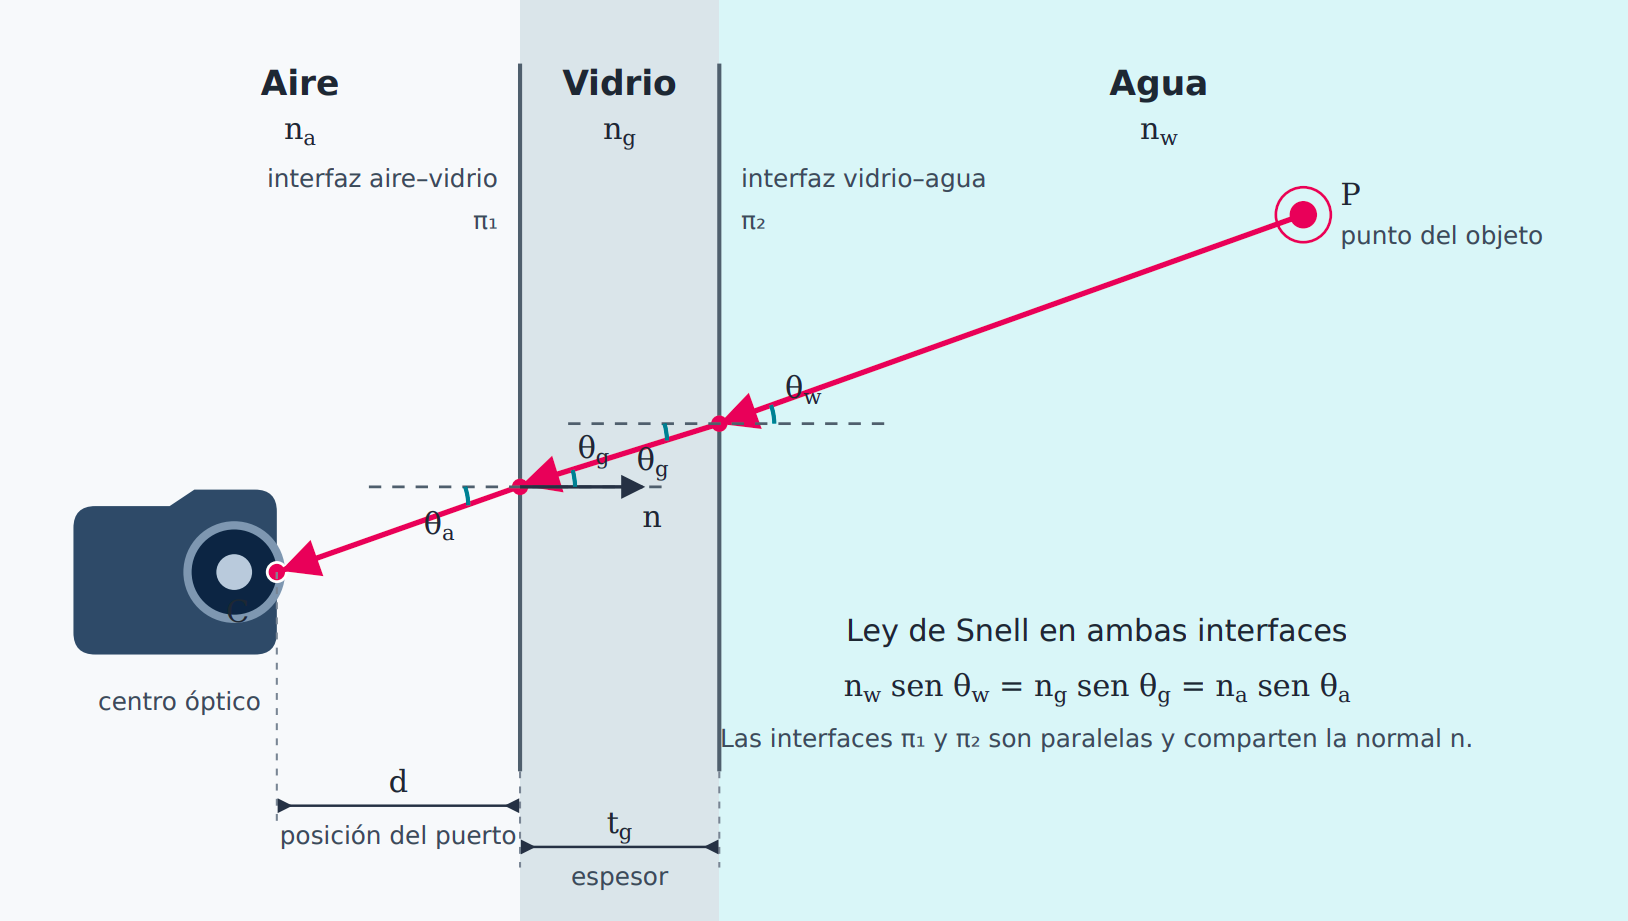
\includegraphics[width=0.9\textwidth]{fig1_1_configuracion.png}
\fignota{Elaboración propia.}
\end{figure}

En este trabajo se evaluaron cuatro procedimientos para convertir píxeles en milímetros, aplicados a los mismos puntos anatómicos de la misma imagen. El primero (A) utiliza la escala de un marcador ArUco adherido al vidrio. El segundo (\Aprime) emplea una homografía calculada con un marcador ubicado en el mismo plano que la réplica. El tercero (B) corresponde a una calibración \emph{pinhole} efectiva realizada bajo el agua. El cuarto (C) modela de forma explícita la desviación de los rayos en el puerto plano. En lugar de peces vivos se utilizaron réplicas rígidas medidas con calibre, de manera que cada estimación pudiera compararse con una longitud conocida. Cuando la profundidad era conocida, se comparó el error de las cuatro rutas; cuando se la consideró desconocida, se empleó C para calcular el intervalo de longitudes compatible con cualquier posición dentro de la pecera y determinar cuánto debe acotarse la profundidad para que ese intervalo resulte útil.



El tema surgió de una pregunta práctica: de qué manera pasar de píxeles a milímetros cuando se quiere medir un pez en una pecera con una cámara convencional. Las respuestas disponibles en la bibliografía son un marcador de escala, una calibración realizada bajo el agua o un modelo óptico explícito, y cada una produce un valor distinto para la misma fotografía. Los trabajos revisados muestran que la refracción afecta la medición \parencite{Agrawal2012,Rofallski2022,Treibitz2012}, pero no comparan el error de estas alternativas sobre los mismos puntos y contra una referencia física cuando la cámara se ubica del lado exterior de un vidrio plano (Sección~\ref{sec:antecedentes}).

Se estudió, por lo tanto, un flujo de medición con una sola cámara y puntos anatómicos marcados a mano sobre fotografías de réplicas rígidas tomadas a través de una pecera de vidrio. Se compararon las cuatro rutas de conversión, A, \Aprime, B y C, sobre los mismos puntos de cada imagen y se evaluó cada una contra la medida física de la réplica. El tema reúne conocimientos de visión por computadora, geometría proyectiva y metrología. Desde la perspectiva de la Ingeniería Informática, el aporte consiste en un procedimiento de medición monocular que declara de forma explícita la incertidumbre que introduce el desconocimiento de la profundidad, y en un módulo de trazado refractivo implementado y verificado experimentalmente.

\section{Enunciado del problema}
\label{sec:enunciado}

\subsection{Planteamiento del problema}

Diversos trabajos han demostrado que de una imagen pueden extraerse tanto los puntos anatómicos de un pez como una referencia de escala, ya sea mediante algoritmos o de forma manual \parencite{Correia2025,Saleh2023,Tseng2020}. Los primeros enfoques se desarrollaron fuera del agua o en montajes controlados. \textcite{Monkman2019} detectaron el pez junto con un marcador ArUco colocado a su lado, aproximadamente en el mismo plano; \textcite{Fernandes2020} segmentaron imágenes de tilapia para extraer medidas corporales; y \textcite{Saleh2023} localizaron puntos anatómicos con fines morfométricos. Estos estudios confirman que las imágenes contienen información morfométrica aprovechable. Muestran también que la correcta ubicación de los puntos no es suficiente para obtener una medida física exacta, y ninguno de ellos considera lo que ocurre cuando la imagen se forma a través de una pared de vidrio y la escala varía con la profundidad.

En condiciones subacuáticas se agrega una dificultad, dado que además de localizar al pez es necesario recuperar su escala o su profundidad. \textcite{AlJubouri2017} resolvieron este problema con dos cámaras ortogonales, y \textcite{Zhou2023} y \textcite{Seibold2026}, mediante visión estéreo y triangulación. MorphoCal emplea una sola cámara, aunque sumergida, y proyecta los puntos sobre un plano de referencia definido mediante una calibración \emph{pinhole} realizada bajo el agua \parencite{Vijayalakshmi2026}. \textcite{Yin2026} corrigieron la refracción en una interfaz aire--agua y analizaron el efecto de suponer distintas profundidades, pero trabajaron con una profundidad nominal y no informaron un intervalo de longitud. Pinax y CalibMar modelan puertos planos, aunque no fueron concebidos para medir peces \parencite{Luczynski2017,Seegraber2025}. En la bibliografía revisada no se encontró una evaluación monocular que compare A, \Aprime, B y C sobre los mismos puntos y que, además, cuantifique el intervalo de longitud cuando la profundidad es desconocida. La Sección~\ref{sec:antecedentes} desarrolla estos antecedentes y los compara en detalle.


La medición a partir de imágenes permitiría reducir la manipulación de los animales y observarlos con mayor frecuencia. El obstáculo es de naturaleza física: cuando la escena atraviesa la interfaz aire--vidrio--agua, la cámara deja de comportarse como una cámara perspectiva simple, y la refracción, sumada a la diferencia de profundidad entre el pez y el marcador de escala, puede producir una longitud aparente distinta de la real aunque los cuatro puntos anatómicos estén correctamente marcados.

La dificultad metodológica consiste en separar tres efectos que suelen presentarse combinados: la escala directa de un marcador adherido al vidrio, la calibración aproximada de una cámara bajo el agua y el modelado explícito de los rayos a través del puerto plano. Para aislarlos, se compararon las rutas A, \Aprime, B y C en la misma imagen y sobre los mismos puntos anatómicos, y se evaluó además la ruta C sobre todo el rango de profundidades físicamente posibles. El resultado de esta última evaluación es un rango geométrico y no un intervalo de confianza estadístico: $[\min_{z} L(z), \max_{z} L(z)]$, es decir, el conjunto de longitudes compatibles con desconocer la posición de $z$ dentro de $[z_{\min}, z_{\max}]$. La notación abreviada $[L(z_{\min}), L(z_{\max})]$ solo es válida cuando $L(z)$ es monótona en ese intervalo.

El estudio se limita a réplicas rígidas vistas de perfil y a dos medidas, la longitud total y la profundidad corporal, esta última tomada sobre el cuerpo y sin incluir las aletas. Los cuatro puntos anatómicos se marcaron a mano una sola vez sobre cada imagen original y se reutilizaron en las cuatro rutas. Las capturas repetidas de una misma réplica se consideran repeticiones técnicas y no unidades experimentales independientes. Esta delimitación permitió aislar el efecto geométrico, a costa de no poder extender las conclusiones de manera directa a peces vivos, en movimiento, en agua turbia, parcialmente ocultos o en posturas distintas de la de perfil.

De esta brecha y de esta delimitación surgen las preguntas que orientaron la investigación.

\subsection{Formulación del problema}

El problema se formula mediante una pregunta principal y dos preguntas secundarias.

\subsubsection*{Pregunta principal}

¿Qué rango de longitudes produce la ruta C al variar la profundidad $z$ dentro del rango físicamente admisible de la pecera y de ventanas acotadas de $\pm 3$ y $\pm 1$~cm, y qué ancho relativo y qué cobertura de la referencia se observan en el montaje experimental?

\subsubsection*{Preguntas secundarias}

\begin{enumerate}
  \item Con $z$ conocida, ¿cómo se comportan A, \Aprime, B y C en longitud total y en profundidad corporal, y cómo cambia el error de A y de B al alejarse de la zona de calibración de B?
  \item ¿Qué sensibilidad tiene la estimación de C a los parámetros geométricos del montaje medidos a mano (distancia cámara--vidrio e índice de refracción del agua)?
\end{enumerate}

\section{Objetivos de la investigación}

\subsection{Objetivo general}

Evaluar, en un montaje controlado con una interfaz aire--vidrio--agua, cuatro estrategias de conversión métrica para estimar con una sola cámara la longitud total y la profundidad corporal de peces, comparándolas sobre los mismos puntos anatómicos contra referencias físicas de réplicas rígidas, y cuantificar con un modelo refractivo de puerto plano el intervalo de longitud que introduce una profundidad desconocida.

\subsection{Objetivos específicos}

\begin{enumerate}
  \item Construir y documentar el conjunto de datos de réplicas, referencias físicas, posiciones, repeticiones y exclusiones.
  \item Establecer un protocolo reproducible de marcado manual de los cuatro puntos anatómicos, único por imagen y compartido por las cuatro rutas.
  \item Implementar y validar las rutas A, \Aprime, B y C, incluido el módulo C de puerto plano, frente a las referencias físicas de las réplicas.
  \item Comparar el error de longitud total y de profundidad corporal de A, \Aprime, B y C sobre las mismas imágenes, y analizar cómo varía ese error con la distancia de la réplica al vidrio.
  \item Calcular el intervalo $[\min_z L(z), \max_z L(z)]$ sobre el rango físicamente admisible de profundidad y sobre ventanas acotadas de $\pm 3$ y $\pm 1$~cm, junto con su ancho relativo y su cobertura.
  \item Evaluar la sensibilidad de las estimaciones de C a las condiciones geométricas del montaje medidas a mano (distancia cámara--vidrio e índice de refracción del agua).
\end{enumerate}

Los objetivos 1, 2 y 3 construyen el conjunto de datos, el protocolo de marcado y las rutas sobre las que se trabaja; el objetivo 4 responde a la pregunta secundaria 1 y se contrasta con las hipótesis H1 y H2; el objetivo 5 responde a la pregunta principal y se contrasta con la hipótesis H3; y el objetivo 6 responde a la pregunta secundaria 2 (Sección~\ref{sec:hipotesis}). Las conclusiones del Capítulo~5 se presentan en ese mismo orden.

\section{Hipótesis}
\label{sec:hipotesis}

Se plantean tres hipótesis de investigación. Los criterios con que se decide cada una se definen en la Sección~\ref{sec:criterios-hipotesis}.

\begin{description}
  \item[H1: comparación geométrica con profundidad conocida.] Con la profundidad conocida, el error absoluto de longitud total de C es menor que el de A, \Aprime{} y B. Responde a la pregunta secundaria 1 y a los objetivos 3 y 4.
  \item[H2: dependencia con la distancia.] La diferencia $\mathrm{error}(B) - \mathrm{error}(C)$ aumenta con la separación respecto de la zona de calibración de B. Responde a la pregunta secundaria 1 y al objetivo 4.
  \item[H3: intervalo por profundidad desconocida.] El intervalo calculado con C, $\IL = [\min_z L(z), \max_z L(z)]$, contiene la longitud física de la réplica cuando $z$ recorre el rango físicamente admisible, y su ancho relativo puede predecirse a partir de la geometría del montaje ($d$, $t_g$, índices y rango de $z$). Responde a la pregunta principal y al objetivo 5.
\end{description}

\section{Justificación}

La medición repetible de los peces permite seguir su crecimiento, estimar el rendimiento y seleccionar ejemplares. En Paraguay la actividad tiene una escala que justifica el interés en el tema, dado que la acuicultura produjo alrededor de 14\,000 toneladas en 2021 \parencite{FAO2025Paraguay}. Un sistema basado en imágenes podría reducir la manipulación directa de los animales y permitir observaciones más frecuentes.

Para la Ingeniería Informática, el interés radica en determinar el límite métrico de un procedimiento con una sola cámara cuando la escena atraviesa un puerto plano. Se mantuvieron fijos la imagen y los cuatro puntos marcados a mano, se compararon A, \Aprime, B y C sobre las mismas observaciones y se hizo explícita la incertidumbre geométrica que agrega la profundidad. El resultado es evidencia experimental que permite decidir en qué condiciones es suficiente una escala directa, cuándo conviene una calibración \emph{pinhole} y cuándo se requiere un modelo refractivo.

La contribución puede verificarse en cinco aspectos: una salida monocular que declara la incertidumbre atribuible a la profundidad; evidencia comparativa de A, \Aprime, B y C en un montaje controlado; una implementación propia del modelo de puerto plano, basada en formulaciones publicadas y evaluada contra referencias físicas; un protocolo reproducible de marcado manual con réplicas rígidas; y un análisis de la sensibilidad de C a los parámetros del montaje medidos a mano.

\section{Delimitación espacial y temporal}
\label{sec:delimitacion}

El trabajo se desarrolló en \Ciudad, Paraguay, sobre un montaje experimental propio: una pecera de vidrio de $30 \times 30 \times 30$~cm, una cámara de teléfono fija y seis réplicas rígidas de peces, descritos en el Capítulo~\ref{cap:metodologia}. Los resultados se refieren a ese montaje. En lo temporal, el trabajo abarcó de agosto a octubre de 2026: armado del montaje y pruebas preliminares en agosto y septiembre, capturas definitivas y calibraciones de cámara en octubre de 2026, y búsqueda de antecedentes cerrada en septiembre de 2026.

\section{Alcance y limitaciones}
\label{sec:alcance}

El trabajo evalúa de forma comparativa cuatro rutas de conversión métrica con una sola cámara y cuantifica la incertidumbre geométrica que introduce una profundidad desconocida. Los resultados corresponden a réplicas rígidas fotografiadas de perfil, en un montaje controlado y con los índices de refracción adoptados en el Capítulo~\ref{cap:metodologia}.

Quedan fuera del alcance los peces vivos, el agua turbia, el movimiento, las oclusiones y las instalaciones productivas. El marcado de los puntos anatómicos es manual, y la repetibilidad del operador no se cuantificó; su posible efecto sobre las medidas se discute en la Sección~\ref{sec:limitaciones}.

\section{Estructura del documento}

El documento consta de cinco capítulos, ordenados según la estructura que establece el reglamento de Proyecto Final de Carrera para una investigación.

\begin{description}
  \item[Capítulo 1. Introducción.] Presenta la motivación, el enunciado del problema con su planteamiento y sus preguntas, los objetivos, las hipótesis, la justificación, la delimitación espacial y temporal, el alcance y las limitaciones, y la estructura del documento.
  \item[Capítulo 2. Marco teórico.] Reúne los antecedentes y la brecha de investigación; el marco referencial, que explica la morfometría, la formación de imágenes a través de una interfaz plana, las rutas A, \Aprime, B y C, el marcado manual, los marcadores ArUco y la evaluación de mediciones; y el marco conceptual, con las definiciones de los términos principales.
  \item[Capítulo 3. Marco metodológico.] Describe el tipo y el enfoque de la investigación, la población y la muestra, las variables con su definición conceptual y operacional, los criterios de decisión de las hipótesis, los instrumentos y técnicas de recolección de datos, los métodos de conversión, el procedimiento, el análisis y la trazabilidad del experimento.
  \item[Capítulo 4. Presentación, análisis e interpretación de resultados.] Presenta los datos y las exclusiones, las calibraciones, la comparación entre A, \Aprime, B y C, el comportamiento según la profundidad, el intervalo por profundidad desconocida, el contraste de hipótesis y la discusión.
  \item[Capítulo 5. Conclusiones y recomendaciones.] Ofrece la regla de decisión que resume el aporte, una conclusión por objetivo, el impacto potencial, las limitaciones, las recomendaciones y el trabajo futuro.
\end{description}

Los anexos reúnen el registro visual de las capturas, los parámetros del puerto plano, los perfiles de calibración, la referencia geométrica del riel, el índice de los repositorios de código y datos, la tabla maestra de resultados, las fichas de las réplicas y las fotografías del montaje y de los instrumentos.

\chapter{Marco teórico}
\label{cap:marco}

La medición de un pez a partir de una fotografía tomada a través de un vidrio requiere encadenar varias etapas, y cada una de ellas puede introducir error. En primer lugar es necesario definir qué se mide y contra qué referencia física; luego, comprender cómo se forma la imagen cuando la luz atraviesa el agua, el vidrio y el aire; y finalmente marcar los puntos anatómicos, recuperar la escala y comparar lo estimado con lo medido. Las etapas de esa cadena se muestran en la Figura~\ref{fig:2-1}, en el mismo orden en que las desarrolla el marco referencial de este capítulo.

Este capítulo tiene tres partes. Primero se revisan los antecedentes y, a partir de ellos, se identifica la brecha que motiva el trabajo (\ref{sec:antecedentes}). Después se desarrolla la teoría de cada etapa de la cadena de medición (\ref{sec:referencial}). Al final se definen los términos que se usan a lo largo del documento (\ref{sec:conceptual}).

\begin{figure}[H]
\centering
\caption[Flujo teórico simplificado de la investigación]{Flujo teórico simplificado de la investigación: escena y referencia física, formación refractiva de la imagen, marcado manual único de puntos, comparación de las rutas A, \Aprime, B y C y evaluación con profundidad conocida o desconocida.}
\label{fig:2-1}
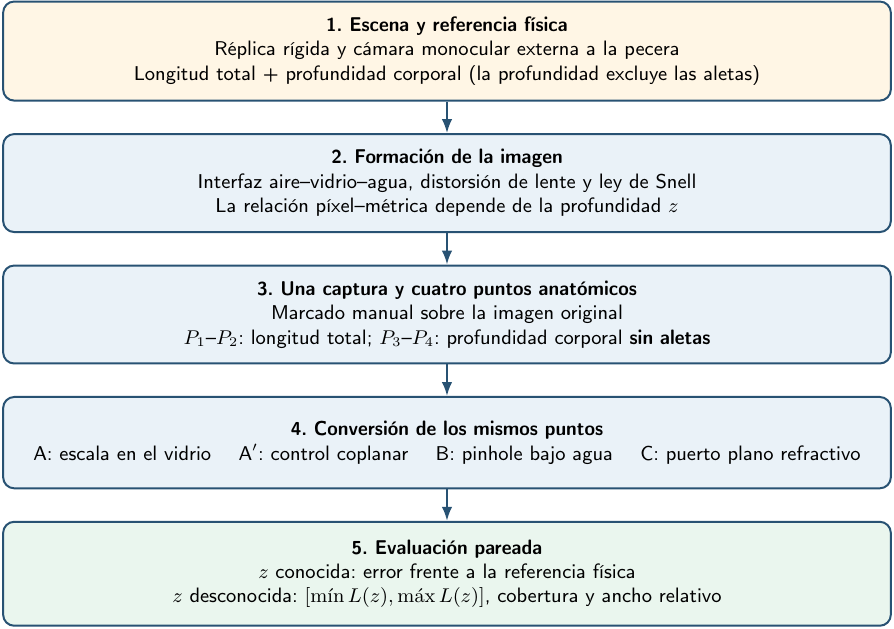
\includegraphics[width=0.85\textwidth]{fig2_1_flujo.png}
\fignota{Elaboración propia.}
\end{figure}

\section{Antecedentes}
\label{sec:antecedentes}

Se realizó una revisión narrativa estructurada de los trabajos sobre medición morfométrica con imágenes, marcado manual o localización de puntos anatómicos, recuperación de escala y formación de imágenes a través de medios refractivos. La búsqueda comenzó con términos generales como «fish measurement», «morphometric analysis», «fish size estimation», «non-invasive measurement» e «image processing», y continuó con combinaciones más específicas: «underwater fish length measurement», «fiducial marker fish measurement», «ArUco fish length», «flat-port camera», «air-glass-water refraction», «refractive camera calibration» y «refraction-aware fish measurement». Las bases consultadas fueron Semantic Scholar y Google Scholar, y la búsqueda se completó siguiendo las referencias de los trabajos encontrados y revisando las fuentes originales. Dado que no se aplicó un protocolo exhaustivo de selección y exclusión, la revisión se considera narrativa y no sistemática. La búsqueda se cerró en septiembre de 2026. Se incluyeron trabajos en español o inglés que trataran al menos uno de estos temas: medición morfométrica de peces con imágenes, recuperación de escala o de puntos anatómicos, calibración de cámaras a través de interfaces aire--vidrio--agua, o modelos explícitos de refracción aplicables a un montaje acuático. Se excluyeron los trabajos sin relación con la medición de organismos acuáticos, la calibración óptica, el marcado de puntos o la estimación de escala, los duplicados y los documentos cuya fuente primaria no pudo identificarse. Además de los catorce trabajos que resume la Tabla~\ref{tab:antecedentes}, se examinaron alrededor de veinte resultados que no se incorporaron a esa matriz.

\textcite{Petrtyl2014} midieron 18 caracteres morfométricos de carpa prusiana de dos maneras, con calibre digital y sobre imágenes, y repitieron las medidas con dos investigadores. Los sesgos relativos medios fueron de $-4{,}27$~\% a $9{,}48$~\%, y en varias comparaciones las diferencias resultaron significativas. Es decir, ni la medición manual ni la digital están libres de sesgo, y ambas cambian según quién mide y cuántas veces. Por eso en este trabajo la referencia manual se tomó con un procedimiento fijo y se la trata como una medida con su propia incertidumbre, no como el valor verdadero.

Sobre la automatización de la información anatómica, \textcite{Petrellis2021} combinó procesamiento de imágenes, detección de contornos, correspondencia de patrones y aprendizaje profundo para estimar la longitud, la profundidad corporal y el área en términos relativos, y para localizar aletas y otras regiones. El error en longitud se ubicó entre 1,9~\% y 13,2~\%. El método trabajó sobre todo con dimensiones relativas, y \citeauthor{Petrellis2021} propuso pasar a visión estéreo, es decir, dos cámaras que observan la misma escena y permiten calcular por triangulación la distancia de cada punto \parencite{Hartley2004}, para obtener dimensiones absolutas en peces inclinados u ocultos.

\textcite{Saleh2023} propusieron MFLD-net, una red liviana que detecta 16 puntos anatómicos en imágenes de peces y, a partir de ellos, calcula la longitud total, la longitud estándar, la longitud cefálica y la profundidad corporal. El modelo logró una precisión promedio de detección $\mathrm{AP} = 0{,}967$ y errores absolutos medios de 9,25~mm en longitud total, 8,27~mm en longitud estándar, 6,57~mm en longitud cefálica y 7,62~mm en profundidad corporal. De este trabajo se tomaron las definiciones de los extremos anatómicos. Su montaje, con cámara industrial y cinta transportadora, es distinto del de esta tesis, donde la imagen se forma a través del vidrio y del agua.

En esta tesis los puntos se marcaron a mano, por dos razones: no atribuirle a un algoritmo una precisión que no se evaluó, y asegurar que las cuatro rutas se comparen sobre exactamente los mismos cuatro puntos. La incertidumbre de la referencia física queda documentada con las tres lecturas de calibre de cada réplica (Tabla~\ref{tab:replicas}).

Un segundo grupo de trabajos se ocupa de la recuperación de la escala. Mediante tres redes regionales, \textcite{Monkman2019} detectaron simultáneamente el pez y un marcador ArUco de tamaño conocido. Calcularon la longitud total a partir del lado mayor de la región detectada y del promedio de las escalas de los cuatro lados del marcador, y reportaron una intersección sobre la unión media cercana al 93~\% y un sesgo porcentual medio de 2,2~\%. También identificaron las principales fuentes de error: la diferencia de profundidad entre marcador y pez, la distorsión de la lente y las orientaciones mayores a unos $20^{\circ}$. Este trabajo respalda el uso de marcadores ArUco y, al mismo tiempo, advierte que el marcador proporciona una escala válida solo si se controlan la coplanaridad y la orientación.

En la misma línea, \textcite{Tseng2020} emplearon una red convolucional para detectar la cabeza, la horquilla caudal y una placa de color de tamaño conocido. Luego ubicaron los puntos del hocico y de la horquilla con procesamiento de imágenes y calcularon la longitud a partir de la relación píxel--distancia de la placa. El clasificador alcanzó una exactitud del 98,78~\%, mientras que la longitud presentó un error absoluto medio de 5,36~cm y un error relativo absoluto medio de 4,26~\%. La diferencia entre ambas cifras muestra que una detección muy precisa no garantiza una medición igualmente precisa.

En un tanque de producción, \textcite{Correia2025} conectaron una cámara a una Raspberry Pi y utilizaron un modelo YOLOv8m-seg para segmentar camarones y una placa de alimentación de tamaño conocido. La placa proporcionó la escala, y la segmentación permitió seleccionar individuos extendidos y aproximadamente coplanares. Obtuvieron un MAPE de 1,56~\% en longitud y de 0,15~\% en anchura. El trabajo integra captura acuática, segmentación y escala visual, pero no corrige la refracción de forma explícita y estudia otro organismo con otra geometría.

Los sistemas estéreo constituyen otra vía para obtener dimensiones físicas. \textcite{Marrable2023} combinaron la detección automática de cabeza y cola con un sistema estéreo BRUVS calibrado con estructuras tridimensionales. Al comparar 3954 mediciones automáticas con mediciones manuales obtuvieron un coeficiente de correlación de Pearson de $r = 0{,}99$. Se trata de una asociación lineal muy fuerte, aunque la correlación no mide concordancia ni descarta un sesgo entre métodos. \textcite{AlJubouri2017}, por su parte, midieron peces cebra a través de un tanque de vidrio con dos cámaras web ortogonales; despreciaron el efecto del vidrio y compensaron la distancia con la segunda vista.

\textcite{ZhangX2025} utilizaron una cámara superior y otra lateral, una red basada en módulos Hourglass y transformaciones tridimensionales para medir siete variables fenotípicas de bagre de canal bajo el agua. El error relativo medio fue de alrededor de 3,7~\% en longitud total y de 9,6~\% considerando las siete variables juntas. El trabajo demuestra que es posible recuperar varias medidas en un montaje acuático, aunque no evalúa por separado el efecto de corregir la refracción.

Los antecedentes de carácter óptico cumplen una función distinta. \textcite{Qiao2019} propusieron un método de estructura a partir del movimiento con un modelo refractivo, capaz de estimar la calibración, la pose de la cámara y la reconstrucción tridimensional a través de superficies que desvían la luz. Con simulaciones e imágenes reales mostraron que ignorar la refracción deforma la reconstrucción. Su objetivo, no obstante, es la reconstrucción de escenas y no la medición de peces.

Para la calibración de cámaras que miran a través de interfaces planas, el modelo Pinax de \textcite{Luczynski2017} representa de forma explícita la refracción en una carcasa de puerto plano y corrige el camino de los rayos antes de reconstruir o medir. Es el antecedente conceptual más cercano a la ruta C, aunque fue concebido como corrección óptica general y no para comparar, en una misma captura monocular, una escala sin corregir, una calibración implícita y un modelo refractivo explícito. En la misma línea, \textcite{Rofallski2022} analizaron la distorsión que depende de la distancia cuando se aplican modelos de cámara convencionales a interfaces multimedia planas, y \textcite{Shortis2015} revisó las técnicas de calibración para medir bajo el agua. Ambos trabajos indican que la compensación implícita depende de la profundidad y que la calidad de una calibración no puede resumirse en un único valor válido para toda la zona de trabajo.

Tres trabajos recientes permiten delimitar con precisión la brecha que aborda esta tesis. MorphoCal \parencite{Vijayalakshmi2026} utiliza una sola cámara, aunque sumergida, y proyecta los puntos sobre un plano de calibración fijo obtenido con un damero bajo el agua; reporta un MAE de 0,75~cm y un RMSE de 0,86~cm sobre 4810 muestras. \textcite{Yin2026} corrigieron la refracción en la superficie agua--aire con la ley de Snell, suponiendo una profundidad nominal (aproximadamente 0,8~m), y analizaron el efecto de ese supuesto, sin informar un intervalo. \textcite{Zhou2023} resolvieron la profundidad con visión estéreo y corrigieron la refracción en la superficie. Ninguno de los tres considera una cámara ubicada del lado exterior de un vidrio plano, ni compara sobre los mismos puntos una escala directa, una calibración implícita y un modelo explícito.

\textcite{Seegraber2025} desarrollaron CalibMar, una herramienta abierta que integra la calibración de la cámara, del par estéreo y de la carcasa para puertos planos o en cúpula. En un puerto plano, el modelo estima la orientación y la posición de la interfaz y representa el camino no central de los rayos. Es un antecedente instrumental, pero no incluye marcado anatómico, referencia ArUco ni evaluación de medidas de peces.

El antecedente más cercano desde el punto de vista óptico es el de \textcite{Seibold2026}, quienes midieron la longitud de pequeños peces de agua dulce en acuarios con una cámara estéreo. Su método combina YOLOv11-Pose, correspondencias restringidas por geometría epipolar refractiva y una triangulación tridimensional que tiene en cuenta las interfaces aire--vidrio--agua. Sus mejores resultados fueron un RMSE de 6,11~mm y 9,22~mm en dos escenas de prueba. El trabajo confirma que la refracción debe incorporarse a la cadena de medición, pero utiliza dos cámaras, no emplea un marcador ArUco y no compara, sobre las mismas observaciones, una cadena con y sin corrección.

La Tabla~\ref{tab:antecedentes} resume las diferencias. Sus cifras no permiten establecer un ordenamiento entre métodos, porque difieren la especie, el tamaño, la geometría, las medidas, los datos e incluso la definición de las métricas.

\begin{landscape}
\pagestyle{apaisada}
\begin{spacing}{1.0}
\begin{footnotesize}
\arrayrulecolor{black!30}
\begin{longtable}{@{}p{2.2cm}p{2.8cm}p{2.6cm}p{3.0cm}p{3.0cm}p{3.2cm}p{3.6cm}@{}}
\caption{Matriz comparativa de antecedentes relacionados con la medición morfométrica y la corrección refractiva.}
\label{tab:antecedentes}\\
\arrayrulecolor{black}\toprule\arrayrulecolor{black!30}
Fuente & Objeto y medio & Geometría & Puntos o procedimiento & Escala y refracción & Medidas y resultados & Limitación frente a este trabajo \\
\arrayrulecolor{black}\midrule\arrayrulecolor{black!30}
\endfirsthead
\multicolumn{7}{l}{\small Tabla~\ref{tab:antecedentes} (continuación)}\\
\arrayrulecolor{black}\toprule\arrayrulecolor{black!30}
Fuente & Objeto y medio & Geometría & Puntos o procedimiento & Escala y refracción & Medidas y resultados & Limitación frente a este trabajo \\
\arrayrulecolor{black}\midrule\arrayrulecolor{black!30}
\endhead
\arrayrulecolor{black}\bottomrule
\endfoot
\endlastfoot
\textcite{Monkman2019} & Lubina europea; fotografías fuera del agua & Monocular; tres cámaras no especializadas & R-CNN para pez y marcador; longitud por región envolvente & ArUco de lado conocido; solo distorsión de lente & LT; mIoU $\approx$ 93~\%; sesgo porcentual medio 2,2~\% & Sin agua ni vidrio; sensible a paralaje, profundidad e inclinación \\
\specialrule{0.3pt}{2pt}{2pt}
\textcite{Tseng2020} & Peces cosechados; fuera del agua & Monocular & CNN para cabeza, horquilla y placa de color & Placa de dimensión conocida; sin refracción & LT; exactitud de clasificación 98,78~\%; MAE 5,36~cm & Fuera del agua; muestra que detectar bien no implica medir bien \\
\specialrule{0.3pt}{2pt}{2pt}
\textcite{Saleh2023} & Peces en cinta transportadora & Cámara industrial monocular en montaje fijo & MFLD-net; 16 puntos anatómicos & Calibración del montaje; sin refracción & LT, LE, cefálica y PC; AP 0,967; MAE 6,57--9,25~mm & Fuera del agua; geometría distinta de un tanque \\
\specialrule{0.3pt}{2pt}{2pt}
\textcite{Correia2025} & Camarones en tanque de producción & Monocular (Raspberry Pi) & YOLOv8m-seg para individuos y placa & Placa como referencia; sin corrección refractiva & Longitud y anchura; MAPE 1,56~\% y 0,15~\% & Objeto y geometría distintos; sin modelo refractivo \\
\specialrule{0.3pt}{2pt}{2pt}
\textcite{AlJubouri2017} & Peces cebra en tanque de vidrio & Dos cámaras web ortogonales & Procesamiento clásico & Compensación de distancia por la segunda vista; vidrio despreciado & Longitud; error $\approx$ 1~\% & Estéreo; no modela el vidrio ni compara rutas \\
\specialrule{0.3pt}{2pt}{2pt}
\textcite{Marrable2023} & Peces en estéreo-BRUVS & Estéreo calibrado & Detección profunda de cabeza y cola & Triangulación estéreo & Longitud; $r = 0{,}99$ frente a manual & Estéreo; correlación no es concordancia \\
\specialrule{0.3pt}{2pt}{2pt}
\textcite{ZhangX2025} & Bagre de canal en agua & Cámaras superior y lateral & Red Hourglass; puntos clave & Transformaciones 3D & Siete variables; ERM 3,7~\% (LT) & Dos vistas; no separa el efecto refractivo \\
\specialrule{0.3pt}{2pt}{2pt}
\textcite{Rofallski2022} & Interfaz plana; análisis de la medición & Modelo convencional a distintas distancias & Patrones de calibración & Distorsión dependiente de la distancia & Error de reproyección & No mide peces; antecedente directo de la validez local de B \\
\specialrule{0.3pt}{2pt}{2pt}
\textcite{Luczynski2017} & Cámaras en carcasa de puerto plano & Modelo Pinax de rayos refractados & Patrones de calibración & Corrección refractiva explícita & Reconstrucción y corrección de imagen & Fundamento óptico de C; sin medidas de peces \\
\specialrule{0.3pt}{2pt}{2pt}
\textcite{Seegraber2025} & Patrones sintéticos y reales & Mono o estéreo con puerto plano o cúpula & Detección de patrones; optimización & Calibración explícita de cámara y carcasa & Parámetros de cámara y puerto & Herramienta de calibración; sin anatomía ni medidas \\
\specialrule{0.3pt}{2pt}{2pt}
\textcite{Vijayalakshmi2026} & Peces en estanques; cámara sumergida & Monocular & Detección y puntos clave (MorphoCal) & Pinhole calibrado bajo agua; proyección rayo--plano & Longitud; MAE 0,75~cm, RMSE 0,86~cm (4810 muestras) & Cámara sumergida; asume un plano de referencia fijo; no evalúa fuera de él \\
\specialrule{0.3pt}{2pt}{2pt}
\textcite{Yin2026} & \emph{Micropterus salmoides} en estanque & Monocular; seguimiento & Puntos clave y fusión de rasgos & Snell en la superficie agua--aire; profundidad nominal $\approx$ 0,8~m & Longitud; sensibilidad al error de profundidad & Interfaz agua--aire sin vidrio; no entrega un intervalo \\
\specialrule{0.3pt}{2pt}{2pt}
\textcite{Zhou2023} & Peces en agua & Estéreo & Puntos clave & Corrección de refracción en la superficie; compara calibrar en aire frente a bajo agua & Longitud; error $\approx$ 1~\% & Estéreo; la profundidad se resuelve con la segunda cámara \\
\specialrule{0.3pt}{2pt}{2pt}
\textcite{Seibold2026} & Peces de arroz en acuario & Estéreo externo a través de aire--vidrio--agua & YOLOv11-Pose; cinco puntos; asociación estéreo & Geometría epipolar y triangulación refractivas & Longitud boca--aleta caudal; RMSE 6,11 y 9,22~mm & Estéreo; sin ArUco; no compara la misma escena con y sin corrección \\
\end{longtable}
\end{footnotesize}
\end{spacing}
\end{landscape}

\pagestyle{membrete}

La matriz muestra que cada componente de la cadena de medición ya fue demostrado, aunque en combinaciones distintas. El marcado de puntos anatómicos y los marcadores o patrones de tamaño conocido permiten recuperar la escala, y los modelos refractivos describen el camino de los rayos a través del puerto. Sin embargo, una buena ubicación de los puntos o una correlación alta no garantizan una aproximación a la medida física, porque el resultado final depende también de la escala, la profundidad, la orientación y el modelo óptico.

Existen sistemas que combinan medición de peces y refracción explícita, como el trabajo estéreo de \textcite{Seibold2026}. Lo que distingue al presente trabajo es la evaluación de una configuración monocular y controlada a través de un puerto plano, con la comparación de A, \Aprime, B y C sobre las mismas escenas, los mismos puntos anatómicos y la misma referencia de escala, y el uso de C para construir $L(z)$ cuando la profundidad es desconocida.

\subsection{Síntesis del estado del arte y brecha de investigación}
\label{sec:brecha}

El estado del arte ha resuelto, por separado, varios componentes de la cadena: el marcado y la detección de puntos anatómicos, la recuperación de escala con marcadores o patrones, la calibración convencional de cámaras y el modelado explícito de la refracción en montajes acuáticos. También hay sistemas estéreo que combinan triangulación y refracción para medir peces.

Lo que permanece abierto, para la configuración estudiada, es qué parte del error de una medición monocular a través de un puerto plano se debe al uso de una escala constante, de una calibración implícita o de una corrección refractiva explícita. En concreto, no se dispone de una comparación pareada que mantenga fijos los puntos marcados, la referencia ArUco y las imágenes; que mida cómo cambia el error al alejarse del plano de calibración; y que establezca qué puede afirmarse sobre la longitud cuando la profundidad no se conoce.

Esta tesis evaluó esa diferencia de forma experimental mediante las rutas A, \Aprime, B y C, la comparación contra una referencia manual y el análisis de la variación del error con la profundidad. El marcado manual es la entrada común; la contribución central es la evaluación geométrica y metrológica de las alternativas de conversión y la medida del intervalo por profundidad desconocida.

No se presenta como novedad un sistema automático de detección anatómica, un marcador nuevo ni un modelo general de calibración refractiva. Tampoco se sostiene que una ruta sea superior en cualquier circunstancia; lo que se afirma es válido para la configuración, las distancias y las condiciones de este experimento.

\section{Marco referencial}
\label{sec:referencial}

El marco referencial reúne la teoría en la que se apoya la medición: qué se mide y contra qué referencia, cómo se forma la imagen a través del vidrio, cómo se convierten los píxeles en milímetros y cómo se evalúa el resultado.

\subsection{Medición morfométrica de peces}

\subsubsection{Morfometría y parámetros corporales}

La morfometría estudia los rasgos externos del tamaño y la forma de un organismo. En peces, estas medidas se obtienen con instrumentos manuales o mediante el análisis de imágenes, y se utilizan para describir la variación corporal y para obtener datos biométricos \parencite{Petrtyl2014}.

En este trabajo se consideran dos medidas: la longitud total y la profundidad corporal. La longitud estándar y la longitud cefálica se excluyeron de manera deliberada, porque el marcado manual permite ubicar sin ambigüedad los extremos de las dos primeras, pero no la placa hipural ni el borde posterior del opérculo que requieren las otras dos. La profundidad corporal se define de forma estricta, para que no se confunda con una dimensión que incluya las aletas.

La longitud total resume el tamaño del pez y se extiende desde la punta del hocico hasta el extremo posterior de la aleta caudal. La profundidad corporal es la distancia entre el perfil dorsal y el perfil ventral del cuerpo, en la sección donde esa separación es máxima, y excluye por completo las aletas dorsal, ventral, pectorales y caudal. Las aletas pueden formar parte de la longitud total cuando constituyen el extremo caudal, pero no intervienen en la profundidad corporal. La referencia física y las cuatro rutas, A, \Aprime, B y C, utilizan exactamente los mismos puntos para ambas medidas, lo que evita seleccionar, una vez observados los datos, la medida que más favorezca a un método.

\subsubsection{Puntos anatómicos y definición de las medidas}
\label{sec:puntos-def}

La medición de longitudes sobre un pez requiere puntos anatómicos que cualquier operador pueda volver a localizar. La bibliografía no siempre utiliza los nombres de manera uniforme, en especial en el caso de la longitud estándar, por lo que se adoptan las siguientes definiciones \parencite{Howe2002,Saleh2023,Steeds2024}:

\begin{description}
  \item[Longitud total (LT):] distancia desde el punto más anterior del hocico hasta el punto más posterior de la aleta caudal, es decir, el extremo del radio caudal más largo. En la práctica se mide como la proyección del segmento entre ambos puntos sobre el eje longitudinal del cuerpo (ecuación~\ref{eq:medidas}); si los dos puntos se ubican sobre el eje, coincide con la distancia en línea recta.
  \item[Profundidad corporal (PC):] mayor distancia dorsoventral entre los perfiles dorsal y ventral del cuerpo, medida en la sección de separación máxima y sin incluir las aletas. Sus extremos se ubican sobre el perfil del cuerpo y no sobre el extremo de una aleta.
\end{description}

Estas definiciones se aplican por igual a la medición con calibre y a la estimación a partir de las imágenes. La longitud estándar y la cefálica quedan como antecedentes o trabajo futuro, porque con los cuatro puntos del marcado manual no es posible observar sus extremos sin ambigüedad. La Figura~\ref{fig:2-2} muestra los puntos y las medidas.

\begin{figure}[H]
\centering
\caption[Puntos anatómicos y medidas morfométricas consideradas]{Puntos anatómicos y medidas morfométricas consideradas. La longitud total incluye el extremo caudal; la profundidad corporal se mide solo sobre el cuerpo y excluye las aletas.}
\label{fig:2-2}
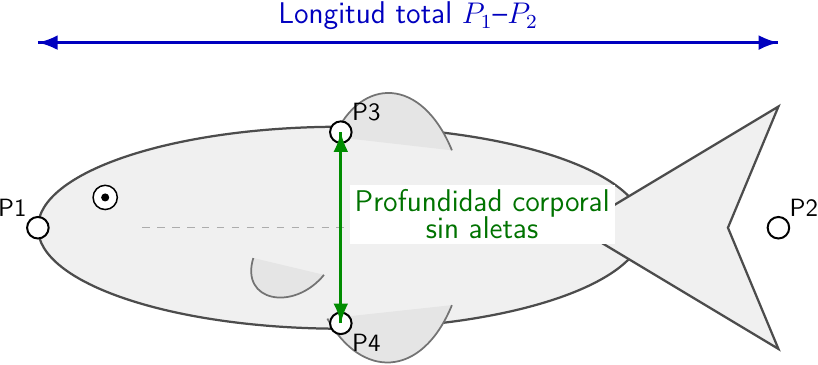
\includegraphics[width=0.8\textwidth]{fig2_2_puntos.png}
\fignota{Elaboración propia.}
\end{figure}

Las medidas tomadas con calibre sobre las réplicas constituyen la referencia contra la cual se evalúa cada estimación. Esta referencia también tiene error, que depende de la resolución del instrumento, de la ubicación de los puntos anatómicos y de la repetibilidad del procedimiento. Por ese motivo se utilizan las mismas definiciones anatómicas en la medición física y en la digital.

\subsubsection{Exactitud, repetibilidad e incertidumbre de la referencia}

La medición manual de un pez no da siempre el mismo resultado: varía entre operadores y entre repeticiones de un mismo operador. Influyen la ubicación de cada punto, la presión del instrumento, la posición del objeto, la resolución del calibre y la experiencia de quien mide \parencite{Petrtyl2014}. El valor manual, por lo tanto, no es un valor exento de incertidumbre, sino una referencia obtenida con un procedimiento controlado.

La exactitud de la referencia indica cuán cerca está del valor real de la magnitud medida; la repetibilidad, cuánto se dispersan las lecturas tomadas en las mismas condiciones. La resolución y la exactitud declaradas del instrumento, la variación entre repeticiones y la elección de los puntos anatómicos agregan incertidumbre a la referencia, y esta debe tenerse presente antes de extraer conclusiones de diferencias pequeñas entre el valor manual y el estimado.

\subsection{Formación de imágenes en medios acuáticos}

\subsubsection{Modelo geométrico convencional de cámara}

El modelo de cámara estenopeica, o \emph{pinhole}, representa la cámara como una caja con un orificio diminuto, de modo que todos los rayos de la escena pasan por ese único punto, el centro de proyección, antes de llegar al plano de la imagen. Con este modelo, la relación entre un punto del espacio, expresado en coordenadas del mundo, y su proyección en la imagen se escribe como \parencite{Hartley2004,Zhang2000}:
\begin{equation}
\lambda \begin{bmatrix} u \\ v \\ 1 \end{bmatrix} = \mathbf{K}\,[\mathbf{R} \mid \mathbf{t}]\begin{bmatrix} X_w \\ Y_w \\ Z_w \\ 1 \end{bmatrix},
\label{eq:pinhole}
\end{equation}
donde $(X_w, Y_w, Z_w)$ son las coordenadas del punto en el sistema del mundo, $(u, v)$ son sus coordenadas en la imagen y $\lambda$ es un factor de escala ligado a la profundidad del punto.

La matriz $\mathbf{K}$ reúne los parámetros intrínsecos, que describen las características internas de la cámara:
\begin{equation}
\mathbf{K} = \begin{bmatrix} f_x & \gamma & c_x \\ 0 & f_y & c_y \\ 0 & 0 & 1 \end{bmatrix},
\label{eq:K}
\end{equation}
donde $f_x$ y $f_y$ son las distancias focales en píxeles, $(c_x, c_y)$ es el punto principal y $\gamma$ recoge una posible falta de perpendicularidad entre los ejes del sensor. Estos parámetros transforman coordenadas de la cámara en coordenadas de la imagen y, en principio, no dependen de la ubicación de la cámara \parencite{Hartley2004}.

Los parámetros extrínsecos, la matriz de rotación $\mathbf{R}$ y el vector de traslación $\mathbf{t}$, describen la posición y la orientación de la cámara. Juntos definen la transformación rígida que lleva las coordenadas del mundo a las de la cámara \parencite{Hartley2004,Zhang2000}.

El modelo \emph{pinhole} es una idealización y no incluye la distorsión que introduce la lente. En una cámara convencional se lo completa con coeficientes de distorsión radial y tangencial. Cuando la imagen se forma a través de interfaces aire--vidrio--agua, en cambio, la refracción modifica además la dirección de los rayos y puede invalidar el supuesto de un único centro de proyección \parencite{Treibitz2012,Seegraber2025}.

\subsubsection{Distorsión óptica producida por la lente}

Una lente real no se comporta como el orificio ideal, sino que desplaza ligeramente la posición de los puntos en la imagen. La formulación habitual describe estos desplazamientos con una componente radial y otra tangencial \parencite{Brown1966,Weng1992}.

Sean $(x, y)$ las coordenadas normalizadas que tendría un punto con una proyección ideal, y sea
\begin{equation}
r^2 = x^2 + y^2,
\end{equation}
donde $r$ es la distancia del punto al eje óptico en el plano normalizado. Las coordenadas distorsionadas, $(x_d, y_d)$, resultan
\begin{equation}
\begin{aligned}
x_d &= x\left(1 + k_1 r^2 + k_2 r^4 + k_3 r^6\right) + 2p_1 xy + p_2\left(r^2 + 2x^2\right),\\
y_d &= y\left(1 + k_1 r^2 + k_2 r^4 + k_3 r^6\right) + p_1\left(r^2 + 2y^2\right) + 2p_2 xy.
\end{aligned}
\label{eq:distorsion}
\end{equation}

Los coeficientes $k_1$, $k_2$ y $k_3$ describen la componente radial. Su efecto crece con la distancia $r$ y se manifiesta principalmente hacia los bordes de la imagen, donde las líneas rectas se curvan en forma de barril o de cojín. Los coeficientes $p_1$ y $p_2$ describen la componente tangencial, o de descentrado, que aparece cuando los elementos de la lente, el eje óptico y el sensor no están perfectamente alineados, y que por ese motivo puede desplazar los puntos de forma asimétrica según la zona de la imagen.

Todos estos coeficientes pertenecen al conjunto cámara--lente. En una calibración convencional se estiman junto con los parámetros intrínsecos, minimizando el error de reproyección bajo el supuesto de una cámara central, es decir, \emph{pinhole} \parencite{Zhang2000}. Con esa compensación la cámara se aproxima a la proyección que produciría una cámara ideal sin distorsión.

La refracción en un puerto plano es un fenómeno distinto. Al atravesar las interfaces aire--vidrio--agua, los rayos dejan de converger, en general, en un único punto, y el sistema se convierte en una cámara axial no central, cuya geometría depende de la orientación y la posición de las interfaces, de sus espesores y de los índices de refracción de cada medio \parencite{Agrawal2012,JordtSedlazeck2012}.

\subsubsection{Refracción en la interfaz aire--vidrio--agua}

Un rayo de luz se desvía al pasar de un medio a otro con distinto índice de refracción. En una interfaz entre dos medios, la ley de Snell relaciona el ángulo de incidencia $\theta_1$, el ángulo refractado $\theta_2$ y los índices de refracción $n_1$ y $n_2$ \parencite{Hecht2017}:
\begin{equation}
n_1 \sin\theta_1 = n_2 \sin\theta_2 .
\label{eq:snell}
\end{equation}

Los ángulos se miden respecto de la normal de la interfaz. En el montaje utilizado, la luz que proviene del objeto atraviesa primero el agua, luego la pared transparente y por último el aire situado frente a la cámara; recorrido en sentido inverso, desde la cámara, el orden es aire, vidrio y agua. La ley de Snell se aplica en cada interfaz, teniendo en cuenta los índices, la orientación de las superficies y su geometría. Como señalan \textcite{Seegraber2025}, una carcasa o un puerto modifica el modelo de formación de la imagen, ya que el camino de cada rayo depende de la forma y la orientación del puerto, de la posición de la cámara respecto de él y de los medios que atraviesa.

\subsubsection{Modelo refractivo de puerto plano}
\label{sec:puerto-plano}

Un puerto plano se modela con dos interfaces paralelas: una entre el aire y la pared transparente, y otra entre la pared y el agua. Para seguir el rayo que corresponde a un píxel conviene recorrerlo desde la cámara hacia la escena. Por el principio de reversibilidad óptica, ese camino coincide con el que recorre la luz desde el objeto hasta la cámara, en sentido contrario \parencite{Agrawal2012,JordtSedlazeck2012}. La Figura~\ref{fig:2-3} muestra la geometría.

\begin{figure}[H]
\centering
\caption[Modelo refractivo de puerto plano]{Modelo refractivo de puerto plano. El centro de la cámara $C$ es el origen; las interfaces $\Pi_1$ (aire--vidrio) y $\Pi_2$ (vidrio--agua) son planos paralelos a distancias $d$ y $d + t_g$ de $C$, con normal común $\mathbf{n}_\pi$. El rayo de un píxel sale de $C$ con dirección $\mathbf{v}_a$, se refracta en $\mathbf{q}_1$ ($\mathbf{v}_g$), atraviesa el vidrio, se refracta de nuevo en $\mathbf{q}_2$ ($\mathbf{v}_w$) y recorre el agua según $\mathbf{X}(\lambda) = \mathbf{q}_2 + \lambda\,\mathbf{v}_w$ (ecuaciones~\ref{eq:q1} a~\ref{eq:rayo}). La línea punteada muestra dónde iría el rayo sin refracción.}
\label{fig:2-3}
\begin{tikzpicture}[scale=0.92,>=Stealth,font=\small]
  % medios
  \fill[gray!22] (4.0,-0.6) rectangle (4.6,5.2);
  \fill[cyan!7]  (4.6,-0.6) rectangle (8.8,5.2);
  \draw[gray!60!black,thick] (4.0,-0.6) -- (4.0,5.2);
  \draw[gray!60!black,thick] (4.6,-0.6) -- (4.6,5.2);
  \node[gray!50!black,above] at (2.0,5.2) {aire, $\mu_a$};
  \node[gray!50!black,above] at (4.3,5.2) {vidrio, $\mu_g$};
  \node[gray!50!black,above] at (7.8,5.2) {agua, $\mu_w$};
  \node[gray!60!black,below] at (4.0,-0.6) {$\Pi_1$};
  \node[gray!60!black,below] at (4.6,-0.6) {$\Pi_2$};
  % eje óptico y normal
  \draw[dashed,gray] (0,0) -- (8.8,0);
  \draw[->,thick] (4.0,0) -- (5.3,0) node[below right=-2pt] {$\mathbf{n}_\pi$};
  % centro de cámara
  \fill (0,0) circle (2.2pt); \node[below left] at (0,0) {$C$};
  % rayo
  \coordinate (q1) at (4.0,2.80);
  \coordinate (q2) at (4.6,3.05);
  \coordinate (X)  at (7.9,4.62);
  \draw[gray,dotted,thick] (q1) -- ++(35:2.6) node[above=2pt,font=\footnotesize,align=center] {rayo sin\\refracción};
  \draw[metC,very thick,->] (0,0) -- (q1);
  \draw[metC,very thick,->] (q1) -- (q2);
  \draw[metC,very thick,->] (q2) -- (X);
  \fill[metC] (q1) circle (2pt); \fill[metC] (q2) circle (2pt); \fill[metC] (X) circle (2.2pt);
  \node[metC,left=3pt] at (q1) {$\mathbf{q}_1$};
  \node[metC,right=3pt] at (q2) {$\mathbf{q}_2$};
  \node[metC,below right=-2pt] at (X) {$\mathbf{X}(\lambda)=\mathbf{q}_2+\lambda\,\mathbf{v}_w$};
  % direcciones
  \node[metC,above left=-2pt,rotate=35] at (2.1,1.5) {$\mathbf{v}_a$};
  \node[metC,above=1pt,rotate=22] at (4.3,2.95) {$\mathbf{v}_g$};
  \node[metC,above left=-2pt,rotate=25] at (6.4,3.9) {$\mathbf{v}_w$};
  % cotas
  \draw[<->] (0,-0.35) -- (4.0,-0.35) node[midway,below] {$d$};
  \draw[<->] (4.0,4.75) -- (4.6,4.75) node[midway,above,font=\footnotesize] {$t_g$};
  \draw[<->] (0,-1.0) -- (4.6,-1.0) node[midway,below] {$d + t_g$};
\end{tikzpicture}
\fignota{Adaptado de \emph{A theory of multi-layer flat refractive geometry}, por A. Agrawal, S. Ramalingam, Y. Taguchi y V. Chari, 2012, \emph{2012 IEEE Conference on Computer Vision and Pattern Recognition}, pp. 3346--3353 (\url{https://doi.org/10.1109/CVPR.2012.6248073}).}
\end{figure}

Se toma el centro de proyección de la cámara como origen de coordenadas y se llama $\mathbf{n}_\pi$ al vector unitario normal a las interfaces, orientado desde la cámara hacia la escena. La cara exterior de la pared (del lado del aire, $\Pi_1$) y la cara interior (del lado del agua, $\Pi_2$) se escriben como
\begin{align}
\Pi_1 &: \mathbf{n}_\pi^{\mathsf{T}}\mathbf{X} = d, \label{eq:pi1}\\
\Pi_2 &: \mathbf{n}_\pi^{\mathsf{T}}\mathbf{X} = d + t_g, \label{eq:pi2}
\end{align}
donde $d$ es la distancia perpendicular entre el centro de la cámara y la primera interfaz, y $t_g$ es el espesor de la pared. Esta representación supone dos superficies planas, paralelas y con la misma normal.

Para un punto de la imagen en coordenadas homogéneas, $\tilde{\mathbf{p}} = (u, v, 1)^{\mathsf{T}}$, ya corregido de la distorsión de la lente, la dirección unitaria del rayo en el aire es
\begin{equation}
\mathbf{v}_a = \frac{\mathbf{K}^{-1}\tilde{\mathbf{p}}}{\lVert \mathbf{K}^{-1}\tilde{\mathbf{p}} \rVert},
\label{eq:va}
\end{equation}
donde $\mathbf{K}$ es la matriz de parámetros intrínsecos de la cámara. El rayo toca la cara exterior del puerto en
\begin{equation}
\mathbf{q}_1 = \frac{d}{\mathbf{n}_\pi^{\mathsf{T}}\mathbf{v}_a}\,\mathbf{v}_a .
\label{eq:q1}
\end{equation}

Para calcular la desviación del rayo al pasar de un medio $i$ a un medio $j$ se utiliza la forma vectorial de la ley de Snell. Si $\mathbf{v}_i$ es la dirección unitaria incidente y $\eta_{ij} = \mu_i/\mu_j$ es el cociente entre los índices de refracción, entonces
\begin{equation}
\mathcal{R}(\mathbf{v}_i; \mu_i, \mu_j, \mathbf{n}_\pi) = \eta_{ij}\left(\mathbf{v}_i - (\mathbf{v}_i^{\mathsf{T}}\mathbf{n}_\pi)\,\mathbf{n}_\pi\right) + \sqrt{1 - \eta_{ij}^2\left(1 - (\mathbf{v}_i^{\mathsf{T}}\mathbf{n}_\pi)^2\right)}\;\mathbf{n}_\pi .
\label{eq:snell-vec}
\end{equation}

Con esta expresión, la dirección del rayo dentro de la pared transparente es
\begin{equation}
\mathbf{v}_g = \mathcal{R}(\mathbf{v}_a; \mu_a, \mu_g, \mathbf{n}_\pi),
\label{eq:vg}
\end{equation}
donde $\mu_a$ y $\mu_g$ son los índices de refracción del aire y del material de la pared. El rayo atraviesa entonces el espesor $t_g$ y sale del vidrio en
\begin{equation}
\mathbf{q}_2 = \mathbf{q}_1 + \frac{t_g}{\mathbf{n}_\pi^{\mathsf{T}}\mathbf{v}_g}\,\mathbf{v}_g .
\label{eq:q2}
\end{equation}

Una segunda aplicación de la ley de Snell, en la interfaz vidrio--agua, proporciona la dirección final del rayo dentro del agua:
\begin{equation}
\mathbf{v}_w = \mathcal{R}(\mathbf{v}_g; \mu_g, \mu_w, \mathbf{n}_\pi),
\label{eq:vw}
\end{equation}
donde $\mu_w$ es el índice de refracción del agua. Todos los puntos de la escena que pueden haber producido ese píxel se encuentran, por lo tanto, sobre el rayo
\begin{equation}
\mathbf{X}(\lambda) = \mathbf{q}_2 + \lambda\,\mathbf{v}_w, \qquad \lambda \geq 0 .
\label{eq:rayo}
\end{equation}
De manera equivalente, un punto $\mathbf{X}$ del espacio compatible con la observación debe cumplir
\begin{equation}
(\mathbf{X} - \mathbf{q}_2) \times \mathbf{v}_w = \mathbf{0}.
\label{eq:restriccion}
\end{equation}

Cada parámetro del puerto tiene un efecto identificable en la imagen. La normal $\mathbf{n}_\pi$ determina la orientación de las interfaces y, con ella, los ángulos de incidencia en cada aplicación de la ley de Snell. Si la normal coincide con el eje óptico, el efecto de la refracción es aproximadamente simétrico alrededor del centro de la imagen; si están desalineados, los rayos se desvían de manera distinta según su posición y esa simetría se pierde.

La distancia $d$ ubica la primera interfaz respecto del centro de la cámara y determina el punto $\mathbf{q}_1$ donde el rayo deja el aire. No modifica el ángulo que impone la ley de Snell, pero desplaza los puntos de intersección y, con ellos, la posición del rayo en el espacio. El espesor $t_g$ tiene un efecto similar, ya que determina la distancia que recorre el rayo dentro de la pared y la separación entre $\mathbf{q}_1$ y $\mathbf{q}_2$.

Los índices $\mu_a$, $\mu_g$ y $\mu_w$ actúan a través de sus cocientes y determinan la desviación del rayo en cada interfaz. Con dos superficies paralelas, el ángulo final del rayo respecto de la normal depende solo de los índices del primer y del último medio; aun así, el índice del vidrio y su espesor influyen en el desplazamiento lateral y en el punto por el que el rayo ingresa al agua.

Dado que cada píxel tiene su propio punto de partida $\mathbf{q}_2$ y su propia dirección $\mathbf{v}_w$, los rayos en el agua no necesariamente se cruzan en un único centro de proyección. Un sistema con interfaces planas y paralelas es, en general, una cámara axial no central, en la que cada rayo se mantiene en el plano formado por el rayo incidente y la normal del puerto \parencite{Agrawal2012}.

\paragraph{Aproximación de primer orden.} Cuando los rayos inciden de forma casi perpendicular al vidrio, la ecuación~\eqref{eq:snell-vec} puede linealizarse y el sistema se comporta como una cámara \emph{pinhole} cuya distancia efectiva al plano del objeto es
\begin{equation}
D(z) = d + \frac{t_g}{\mu_g} + \frac{z}{\mu_w},
\label{eq:Dz}
\end{equation}
donde $z$ es la profundidad del objeto detrás de la cara interior del vidrio. La magnificación de un objeto a profundidad $z$ es proporcional a $1/D(z)$, de modo que el tamaño aparente disminuye con la distancia. Esta relación no reemplaza al trazado completo, pero es suficiente para predecir el signo y el orden de magnitud del error de una escala tomada en el vidrio, así como el ancho del intervalo que produce el desconocimiento de la profundidad. En el Capítulo~\ref{cap:resultados} se contrastan ambas predicciones con los datos.

\subsubsection{Profundidad, inclinación y acortamiento aparente}

La posibilidad de recuperar medidas físicas a partir de una imagen depende de la ubicación relativa de la cámara, la pared transparente, el objeto y la referencia métrica. Detrás de una pared plana, la posición y el tamaño aparente del objeto cambian con su profundidad y con su ubicación en el campo de visión \parencite{Hartley2004,Treibitz2012}.

Para que una medida observada represente adecuadamente al objeto, su plano lateral debe ser aproximadamente paralelo a la pared. Si el objeto gira fuera de ese plano, sus dimensiones proyectadas se acortan. Algo similar ocurre si el eje longitudinal se inclina, porque cambia la orientación de la medida en la imagen y resulta más difícil ubicar los puntos anatómicos.

Una escala obtenida de una referencia visual solo puede trasladarse al objeto si ambos se encuentran en condiciones geométricas equivalentes. Si el marcador y la réplica están a profundidades distintas, la perspectiva y la refracción les asignan escalas aparentes distintas \parencite{Monkman2019}, como muestra la Figura~\ref{fig:2-5}.

\begin{figure}[H]
\centering
\caption[Escala aparente de un marcador según su profundidad]{Un marcador fijo en el vidrio y una réplica situada a profundidad $z$ se observan con magnificaciones distintas: la escala del marcador (rojo) no se transfiere a la réplica (verde). Un marcador coplanar con la réplica (naranja) comparte su magnificación.}
\label{fig:2-5}
\begin{tikzpicture}[scale=0.9,>=Stealth,font=\small]
  % vidrio
  \fill[gray!25] (2.0,-0.3) rectangle (2.3,3.3);
  \node[gray!70!black,above] at (2.15,3.3) {vidrio};
  \fill[cyan!8] (2.3,-0.3) rectangle (10.6,3.3);
  % cámara
  \node[draw,fill=white,minimum width=0.9cm,minimum height=0.6cm] (cam) at (0.2,1.5) {};
  \fill (0.65,1.5) circle (1.5pt);
  \node[below] at (0.2,1.2) {cámara};
  % marcador en el vidrio
  \draw[very thick,metA] (2.35,1.0) -- (2.35,2.0);
  \node[metA,left,align=right] at (1.95,2.5) {marcador\\en el vidrio};
  % marcador coplanar y pez
  \draw[very thick,metAp] (6.2,0.5) -- (6.2,1.5);
  \draw[very thick,metC] (6.2,1.7) -- (6.2,2.9);
  \node[metAp,right,align=left] at (6.3,1.0) {marcador\\coplanar};
  \node[metC,right] at (6.3,2.3) {réplica (LT)};
  % rayos extremos del marcador en vidrio
  \draw[metA] (0.65,1.5) -- (2.35,1.0);
  \draw[metA] (0.65,1.5) -- (2.35,2.0);
  % rayos de la réplica: aire hasta vidrio, luego quebrados
  \draw[metC] (0.65,1.5) -- (2.0,1.62) -- (2.3,1.645) -- (6.2,1.7);
  \draw[metC] (0.65,1.5) -- (2.0,2.33) -- (2.3,2.40) -- (6.2,2.9);
  % anotación
  \draw[<->] (2.3,-0.15) -- (6.2,-0.15) node[midway,below] {$z$ (profundidad desconocida)};
  \node[align=left,font=\footnotesize,anchor=west] at (8.35,1.0) {misma longitud,\\distinto tamaño\\aparente};
\end{tikzpicture}
\fignota{Elaboración propia.}
\end{figure}

La ubicación de la cámara, el tamaño y el material del tanque, las distancias de trabajo, la posición del marcador y las tolerancias de postura, inclinación y diferencia de profundidad son decisiones del diseño experimental. El Capítulo~\ref{cap:metodologia} detalla estos valores y el esquema del montaje.

\subsubsection{Profundidad conocida y profundidad desconocida}
\label{sec:z-desconocida}

La profundidad $z$ es la distancia entre el objeto y la referencia geométrica del montaje, medida desde la cara interna del vidrio o en el sistema de coordenadas de la calibración. Se considera conocida cuando un soporte fija y mide la posición de la réplica. En ese caso, cada rayo se interseca con el plano del objeto, se obtiene una estimación puntual y es posible comparar A, \Aprime, B y C contra la referencia física.

Se considera desconocida cuando una sola imagen no permite determinar a qué distancia del vidrio se encuentra el pez. En ese caso se evalúa C sobre todo el rango físicamente posible, $z \in [z_{\min}, z_{\max}]$. Si $L(z)$ es la longitud que se obtiene al suponer la profundidad $z$, el intervalo geométrico es
\begin{equation}
\IL = \Big[\min_{z \in [z_{\min}, z_{\max}]} L(z),\ \max_{z \in [z_{\min}, z_{\max}]} L(z)\Big].
\label{eq:IL}
\end{equation}

La forma abreviada $[L(z_{\min}), L(z_{\max})]$ solo es equivalente si $L(z)$ es monótona en el rango. En la aproximación de primer orden de la ecuación~\eqref{eq:Dz}, $L(z)$ es proporcional a $D(z)$ y, por lo tanto, crece con $z$; en el Capítulo~\ref{cap:resultados} se verifica con el trazado completo. El intervalo expresa únicamente la incertidumbre debida a la profundidad desconocida. No incluye los errores de calibración, de postura, de marcado manual ni de la referencia de calibre, que se informan por separado (Secciones~\ref{sec:calibraciones} y~\ref{sec:sensibilidad} y Tabla~\ref{tab:replicas}); la repetibilidad del marcado no se cuantificó. No debe interpretarse como un intervalo de confianza.

\subsubsection{Calibración y corrección refractiva}

CalibMar, el software de \textcite{Seegraber2025}, calibra cámaras y carcasas con puertos planos o en cúpula, y estima tanto los parámetros intrínsecos como los de la geometría refractiva. En este trabajo opera como antecedente instrumental, ya que los perfiles de calibración se obtuvieron con la rutina \texttt{calibrateCamera} de OpenCV \parencite{Zhang2000}, y la ruta C utiliza el trazado de rayos implementado en la aplicación desarrollada en este trabajo (Sección~\ref{sec:metodos}).

Para medir el efecto geométrico se aplican las cuatro rutas, A, \Aprime, B y C, a la misma escena. Si la imagen, el criterio de marcado, los puntos anatómicos y la referencia física se mantienen fijos, las diferencias de error pueden atribuirse con mayor claridad al tratamiento geométrico. La salida de una herramienta de calibración no es, por sí misma, una «corrección refractiva», ni puede convertirse sin verificación en coeficientes de distorsión de lente. La ruta C requiere parámetros, unidades, un sistema de coordenadas y un trazado coherentes con la geometría del montaje; por ese motivo se documentan los parámetros que consume, sus unidades y el sistema de coordenadas que utiliza.

\subsection{Estrategias de conversión métrica A, \Aprime, B y C}
\label{sec:rutas}

El experimento compara cuatro rutas geométricas aplicadas a los mismos puntos de cada imagen. La Figura~\ref{fig:2-4} las presenta de forma comparada.

\begin{figure}[H]
\centering
\caption[Las cuatro rutas de conversión métrica lado a lado]{Las cuatro rutas de conversión métrica sobre la misma escena. A toma la escala de un marcador en el vidrio y supone rayos rectos; \Aprime{} rectifica el plano del marcador coplanar con la réplica; B usa una cámara \emph{pinhole} con parámetros efectivos ajustados bajo el agua; C traza cada rayo a través de aire, vidrio y agua.}
\label{fig:2-4}
\begin{tikzpicture}[scale=0.6,>=Stealth,font=\scriptsize]
\foreach \x/\lab/\col/\txt in {0/A/metA/{escala del marcador\\en el vidrio},
                               6.4/\Aprime/metAp/{homografía del marcador\\coplanar con la réplica},
                               12.8/B/metB/{pinhole efectivo\\calibrado bajo el agua},
                               19.2/C/metC/{rayo refractado dos veces\\(puerto plano)}}{
  \begin{scope}[shift={(\x,0)}]
    \fill[gray!25] (1.6,0) rectangle (1.85,3.6);
    \fill[cyan!8] (1.85,0) rectangle (5.6,3.6);
    \node[draw,fill=white,minimum width=0.6cm,minimum height=0.45cm] at (0.3,1.8) {};
    \fill (0.6,1.8) circle (1.2pt);
    \draw[very thick,metC] (4.6,1.2) -- (4.6,2.6);
    \node[\col,font=\bfseries\small] at (2.8,4.1) {\lab};
    \node[align=center,font=\scriptsize] at (2.8,-0.55) {\txt};
  \end{scope}
}
% A: marcador en vidrio y rayos rectos
\draw[very thick,metA] (1.9,1.5) -- (1.9,2.1);
\draw[metA,dashed] (0.6,1.8) -- (4.6,1.2); \draw[metA,dashed] (0.6,1.8) -- (4.6,2.6);
% A': marcador junto a la réplica
\draw[very thick,metAp] (6.4+4.2,0.9) -- (6.4+4.2,1.5);
\draw[metAp,dashed] (6.4+0.6,1.8) -- (6.4+4.6,1.2); \draw[metAp,dashed] (6.4+0.6,1.8) -- (6.4+4.6,2.6);
% B: pinhole recto con damero
\foreach \i in {0,1,2}{\foreach \j in {0,1}{\fill[black!60] (12.8+2.3+\i*0.22,0.4+\j*0.22) rectangle ++(0.22,0.22);}}
\draw[metB] (12.8+0.6,1.8) -- (12.8+4.6,1.2); \draw[metB] (12.8+0.6,1.8) -- (12.8+4.6,2.6);
% C: rayos quebrados
\draw[metC] (19.2+0.6,1.8) -- (19.2+1.6,1.62) -- (19.2+1.85,1.6) -- (19.2+4.6,1.2);
\draw[metC] (19.2+0.6,1.8) -- (19.2+1.6,2.3) -- (19.2+1.85,2.34) -- (19.2+4.6,2.6);
\end{tikzpicture}
\fignota{Elaboración propia.}
\end{figure}

\begin{description}
  \item[A: escala directa en el vidrio.] El marcador ArUco queda pegado a la pared y su tamaño conocido convierte píxeles en milímetros. Constituye la línea de base más realista, la que emplearía cualquier usuario con una cámara y un marcador, pero está afectada por el paralaje: si la réplica se encuentra a otra profundidad, su escala aparente es distinta.
  \item[\Aprime: escala aproximadamente coplanar.] El marcador se coloca en el mismo plano de profundidad que la réplica, dentro de la tolerancia que fija la metodología. Esta ruta permite medir cuánto del error de A se debe a la separación entre marcador y objeto. Como rectifica el plano con una homografía, la diferencia entre A y \Aprime{} combina dos efectos: la coplanaridad y la corrección de perspectiva del plano del marcador.
  \item[B: cámara \emph{pinhole} calibrada bajo el agua.] Calibrar la cámara con un patrón visto a través del mismo sistema aire--vidrio--agua compensa la refracción de forma implícita: el ajuste elige parámetros intrínsecos y coeficientes de distorsión efectivos que minimizan el error de reproyección en la zona que cubren las imágenes de calibración. Esta calibración se realizó en la posición más cercana al vidrio y el error se estudió según la separación respecto de esa zona. La parametrización no reproduce la geometría no central de un puerto plano, pero puede aproximarla adecuadamente si se mide a distancias similares a las de la calibración \parencite{JordtSedlazeck2012,Treibitz2012,Shortis2015}. La limitación es que la compensación necesaria cambia con la distancia entre la cámara y el punto observado, de modo que un único conjunto de parámetros \emph{pinhole} no describe con la misma calidad objetos a distintas profundidades. Las simulaciones de \textcite{Rofallski2022} muestran que la calibración implícita funciona mejor cerca de la distancia de calibración y pierde exactitud al alejarse, y que se degrada aún más si el eje óptico no es perpendicular a la interfaz. La hipótesis H2 se apoya en ese comportamiento.
  \item[C: puerto plano explícito.] Cada rayo se sigue a través de las interfaces con la ley de Snell y las dimensiones se recuperan para una profundidad supuesta. Al recorrer una grilla de valores admisibles de $z$ se obtiene $L(z)$ y, cuando $z$ es desconocida, el intervalo geométrico $[\min_z L(z), \max_z L(z)]$. La ruta C no aísla la refracción como única causa, sino que incorpora el modelo completo de interfaces y la información de profundidad, lo que se tiene en cuenta al interpretar sus resultados.
\end{description}

El marcado manual, la imagen y la referencia física son los mismos para las cuatro rutas. En consecuencia, una diferencia entre métodos no puede atribuirse a una elección distinta de puntos ni a una imagen rectificada.

\subsection{Marcado manual de puntos anatómicos}

A diferencia de los trabajos de la Sección~\ref{sec:antecedentes}, que localizan los puntos anatómicos con redes neuronales, en este proyecto los cuatro puntos de cada captura se marcaron a mano sobre la imagen original, con un criterio anatómico fijo: $\mathbf{p}_1$ y $\mathbf{p}_2$ son los extremos de la longitud total, y $\mathbf{p}_3$ y $\mathbf{p}_4$, los de la profundidad corporal, sin incluir ninguna aleta.

Cada captura se marcó una sola vez y las mismas coordenadas se reutilizaron en A, \Aprime, B y C. Cada registro de medición conserva la réplica, la imagen, el operador, la fecha, el criterio aplicado y cualquier revisión. Un nuevo marcado, o una revisión independiente, permite estimar la repetibilidad del procedimiento, pero no lo convierte en una salida automática ni genera una nueva unidad experimental.

La incertidumbre de la ubicación manual de los puntos se separa de la incertidumbre geométrica por profundidad. Quedaron registrados los casos en que el contorno, la postura o la visibilidad de una aleta dificultaron la ubicación de un punto, así como el motivo de cada exclusión. Esta separación permite atribuir las diferencias entre A, \Aprime, B y C al tratamiento geométrico, dado que los puntos anatómicos son siempre los mismos.

\subsection{Recuperación de la escala física}

\subsubsection{Marcadores fiduciales ArUco}

Los marcadores ArUco son cuadrados con un borde negro y una matriz interna de celdas blancas y negras, cuyo patrón binario identifica a cada marcador. Al detectarlo, el algoritmo entrega su identificador y la posición de sus cuatro esquinas en la imagen. Si se conoce el tamaño real del marcador, esas esquinas vinculan la imagen con el mundo físico \parencite{GarridoJurado2014}.

En una escena frontal y casi plana, el tamaño aparente del marcador proporciona una escala local entre píxeles y milímetros. Si además se conocen los parámetros intrínsecos y de distorsión de la cámara, es posible estimar la pose del marcador respecto de ella. Por último, con las cuatro esquinas y sus posiciones conocidas en el plano puede construirse una homografía que rectifique ese plano. Las tres opciones no son equivalentes, porque la escala directa supone una magnificación casi uniforme, la pose depende del modelo de cámara y la homografía solo es válida para puntos situados en el mismo plano.

El diccionario, el identificador, el tamaño físico, la forma de cálculo elegida y las reglas para aceptar o descartar una detección son parámetros del sistema; el Capítulo~\ref{cap:metodologia} los documenta.

\subsubsection{Conversión entre píxeles y unidades físicas}

En una escena frontal y casi plana, el tamaño conocido del marcador proporciona una escala local. Sea $L_m$ la longitud física de su lado y sean $p_i$, con $i = 1, \ldots, 4$, las longitudes en píxeles de sus cuatro lados detectados. Cada una se calcula a partir de dos esquinas consecutivas:
\begin{equation}
p_i = \sqrt{(x_{i+1} - x_i)^2 + (y_{i+1} - y_i)^2},
\label{eq:lado}
\end{equation}
donde, para cerrar el contorno, se toma $(x_5, y_5) = (x_1, y_1)$.

\textcite{Monkman2019} estiman la cantidad de milímetros que representa un píxel promediando las escalas de los cuatro lados del marcador:
\begin{equation}
k = \frac{1}{4}\sum_{i=1}^{4}\frac{L_m}{p_i},
\label{eq:escala-monkman}
\end{equation}
donde $k$ queda en unidades físicas por píxel, por ejemplo mm/píxel. El promedio de los cuatro lados reduce la dependencia de una sola detección y absorbe las pequeñas diferencias entre las longitudes observadas en la imagen. La implementación utilizada divide el lado físico por el promedio de los cuatro lados en píxeles (Sección~\ref{sec:metodos}); para marcadores correctamente detectados, ambas variantes difieren en menos de una centésima de píxel.

Si $d_f$ es la distancia en píxeles entre dos puntos anatómicos, la longitud física estimada es
\begin{equation}
\hat{L}_f = k\,d_f .
\label{eq:Lf}
\end{equation}

\textcite{Monkman2019} emplearon este procedimiento para estimar la longitud total de peces con marcadores ArUco de tamaño conocido. El método supone que la magnificación es la misma en el marcador y en la región medida, lo que exige que ambos se encuentren aproximadamente en el mismo plano y con una orientación similar respecto de la cámara. Si están a distinta profundidad, aparece una diferencia de escala que esta relación no corrige.

Además, las esquinas del marcador y los puntos anatómicos deben expresarse en el mismo sistema de coordenadas y en la misma condición de corrección de la imagen. El Capítulo~\ref{cap:metodologia} indica en qué etapa del procesamiento se obtiene la escala y cómo se revisa el marcado.

\subsubsection{Homografía y perspectiva}

Una homografía es la transformación proyectiva que relaciona las coordenadas de un plano con las de su imagen, y se representa con una matriz de $3 \times 3$ \parencite{Hartley2004}. Rectifica únicamente el plano que la define: no recupera la posición espacial de los puntos situados fuera de ese plano, ni corrige la diferencia de escala que aparece cuando el marcador y el pez se encuentran a distinta profundidad. En presencia de refracción, además, la homografía es una aproximación, ya que puede ajustar adecuadamente las correspondencias del plano de referencia sin representar el camino de todos los rayos aire--vidrio--agua. La Sección~\ref{sec:metodos} presenta la homografía que usa \Aprime.

\subsection{Estimación y evaluación morfométrica}

Para evaluar una medición conviene distinguir tres propiedades. La exactitud indica cuán cerca se encuentra una estimación de la referencia física; la repetibilidad, cuánto se dispersan las repeticiones técnicas en las mismas condiciones; y la concordancia, si dos procedimientos producen valores comparables, lo que es una condición más exigente que la correlación \parencite{Bland1986,Lin1989}. Las tres propiedades se examinan sobre las mismas réplicas, con errores con signo y absolutos, métricas agregadas y análisis pareados.

La referencia manual se trata como una medición controlada que también tiene incertidumbre. Por ese motivo, MAE, RMSE y MAPE se interpretan como diferencias respecto de esa referencia, y el sesgo se utiliza para detectar tendencias sistemáticas. Las repeticiones de una misma réplica se resumieron antes de cualquier comparación inferencial, porque no son unidades experimentales independientes. Las definiciones, fórmulas, agregaciones y criterios de decisión están en el Capítulo~\ref{cap:metodologia}.

\subsubsection{Trazabilidad de la medición}

Para que una medición pueda reproducirse, cada resultado debe guardar, junto con el valor estimado, la imagen de origen, el modo de corrección, el perfil de calibración, el marcador usado, el protocolo de marcado, el operador, la unidad y las advertencias de calidad. Con esa información se puede reconstruir el camino completo, desde la captura hasta la comparación con la referencia, y determinar si un error proviene de la adquisición, la corrección, el marcado o la conversión métrica.

Los datos mínimos que entrega cada medición, la estructura del archivo JSON y las evidencias que se conservan para su inspección son decisiones de diseño e implementación. El Capítulo~\ref{cap:metodologia} las define y describe la trazabilidad efectiva entre los datos de entrada, los resultados y las evidencias.

\section{Marco conceptual}
\label{sec:conceptual}

Esta sección establece el sentido con que se emplean los términos principales del trabajo. Las definiciones resumen lo desarrollado en el marco referencial y en el Capítulo~\ref{cap:metodologia}.

\begin{description}
  \item[Morfometría.] Medición de las dimensiones y de la forma externa del cuerpo de un organismo. En este trabajo se reduce a dos medidas: la longitud total y la profundidad corporal.
  \item[Punto anatómico.] Lugar del cuerpo que puede ubicarse de forma repetible en la réplica y en la imagen. Se utilizan cuatro, de $\mathbf{p}_1$ a $\mathbf{p}_4$ (Sección~\ref{sec:puntos-def}).
  \item[Longitud total (LT).] Distancia entre el extremo anterior del hocico y el punto más posterior de la aleta caudal, medida sobre el eje longitudinal del pez.
  \item[Profundidad corporal (PC).] Distancia entre el perfil dorsal y el ventral en una misma sección transversal del cuerpo, sin incluir las aletas.
  \item[Réplica rígida.] Modelo de pez impreso en PLA cuyas dimensiones no cambian. Sus medidas con calibre son la referencia física de cada estimación.
  \item[Conversión métrica.] Transformación que lleva las coordenadas de un punto de la imagen, en píxeles, a milímetros. A, \Aprime, B y C son cuatro conversiones distintas (Sección~\ref{sec:rutas}).
  \item[Marcador ArUco.] Cuadrado de lado conocido con un código binario que un detector localiza automáticamente en la imagen \parencite{GarridoJurado2014}. Sus esquinas sirven como referencia de escala.
  \item[Homografía.] Transformación proyectiva entre dos planos, representada por una matriz de $3 \times 3$ \parencite{Hartley2004}. Corrige la perspectiva de los puntos que pertenecen al plano que la define.
  \item[Visión estéreo.] Técnica que recupera la posición tridimensional de un punto a partir de dos imágenes de la misma escena tomadas desde posiciones conocidas: la diferencia entre ambas imágenes permite triangular la distancia del punto a las cámaras \parencite{Hartley2004}. Requiere dos cámaras; en este trabajo se utiliza una sola.
  \item[Calibración de cámara.] Estimación de los parámetros intrínsecos de la cámara y de los coeficientes de distorsión de la lente a partir de imágenes de un patrón conocido, como un damero \parencite{Zhang2000}.
  \item[Modelo \emph{pinhole} efectivo.] Modelo de cámara \emph{pinhole} calibrado con el patrón bajo el agua. Incorpora de forma empírica el efecto de la refracción, sin representarla explícitamente, y es la base del método B.
  \item[Refracción e índice de refracción.] La refracción es el cambio de dirección de la luz al pasar de un medio a otro. El índice de refracción de cada medio determina la magnitud de la desviación, según la ley de Snell (ecuación~\ref{eq:snell}; \cite{Hecht2017}).
  \item[Puerto plano.] Pared transparente y plana que separa la cámara del agua. Se modela como dos interfaces paralelas, aire--vidrio y vidrio--agua (Sección~\ref{sec:puerto-plano}).
  \item[Profundidad $z$.] Distancia entre el plano de simetría de la réplica y la cara interna del vidrio. Es conocida cuando un soporte la fija, y desconocida cuando una sola imagen no permite determinarla (Sección~\ref{sec:z-desconocida}).
  \item[Intervalo geométrico $\IL$.] Rango de longitudes compatibles con todas las profundidades admisibles (ecuación~\ref{eq:IL}). Expresa la incertidumbre debida al desconocimiento de $z$ y no es un intervalo de confianza estadístico.
  \item[Exactitud y repetibilidad.] La exactitud indica cuán cerca está una medida del valor real; la repetibilidad, cuánto se dispersan las lecturas tomadas en las mismas condiciones.
\end{description}

\chapter{Metodología}
\label{cap:metodologia}

Este capítulo cuenta cómo medimos réplicas rígidas de peces a partir de fotografías tomadas a través de una pecera. La investigación es aplicada, cuantitativa y usa un diseño experimental pareado. Pareado significa que cada imagen, con sus mismos puntos anatómicos, pasó por los cuatro métodos de conversión métrica: cualquier diferencia entre ellos se debe al método y no a la foto.

\section{Tipo de investigación, enfoque, población y muestra}
\label{sec:diseno}

Se trata de una investigación aplicada, cuantitativa y experimental, con diseño pareado: cada unidad experimental recibe los cuatro tratamientos (A, \Aprime, B y C) sobre la misma observación. La población objetivo son las imágenes de peces tomadas a través de un vidrio plano con una cámara externa. La muestra no es probabilística: son las 72 imágenes de las seis réplicas rígidas disponibles, fotografiadas a cuatro profundidades con tres capturas por condición.

La unidad experimental es una réplica rígida de pez, y la unidad de observación, una medición obtenida de una fotografía. Usamos seis réplicas, R1--R6, impresas en PLA y de tamaños distintos (Figura~\ref{fig:3-1}). La especie que imitan no es una variable del estudio: buscamos variedad de formas y longitudes. Medimos con calibre las dimensiones de referencia de cada réplica y las registramos en el archivo maestro del experimento (Tabla~\ref{tab:replicas}).

\begin{figure}[htbp]
\centering
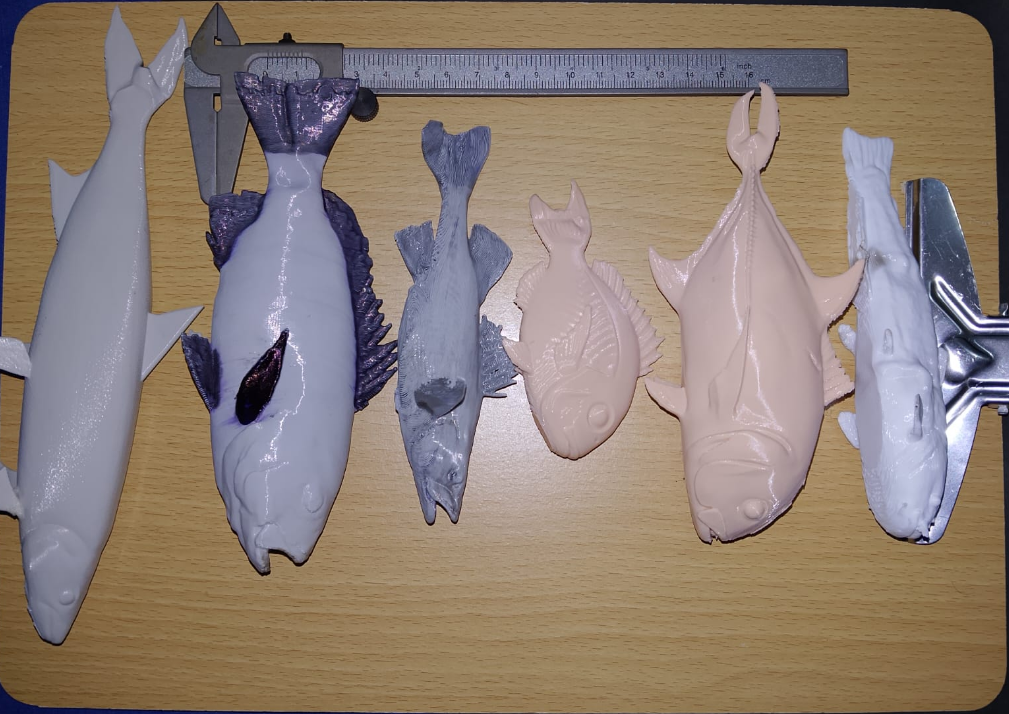
\includegraphics[width=0.8\textwidth]{fig3_1_replicas.png}
\caption[Réplicas de peces impresas en PLA utilizadas en el experimento]{Réplicas de peces impresas en PLA utilizadas en el experimento. Fuente: elaboración propia.}
\label{fig:3-1}
\end{figure}

\begin{table}[htbp]
\centering\footnotesize
\caption{Réplicas y referencias físicas medidas con calibre.}
\label{tab:replicas}
\begin{tabular}{@{}lp{1.6cm}p{1.5cm}p{1.6cm}p{1.5cm}@{}}
\toprule
Réplica & LT media (mm) & Desv. LT (mm) & PC media (mm) & Desv. PC (mm) \\
\midrule
R1 & 158,7 & 1,5 & 45,0 & 0,0 \\
R2 & 134,3 & 2,9 & 27,3 & 0,6 \\
R3 & 91,7 & 0,6 & 40,3 & 0,6 \\
R4 & 142,7 & 2,9 & 42,7 & 0,6 \\
R5 & 137,3 & 0,6 & 25,7 & 0,6 \\
R6 & 209,7 & 0,6 & 35,3 & 0,6 \\
\bottomrule
\end{tabular}
\end{table}

Tomamos cada medida de referencia tres veces con un calibre analógico con nonio (Figura~\ref{fig:H-2}) y registramos las lecturas al milímetro. La media es la referencia; la desviación estándar muestral entre lecturas indica cuán repetible es (Tabla~\ref{tab:replicas}). La mayor desviación fue de 2,9~mm, en la LT de R2 y R4; en PC no pasó de 0,6~mm. Estas desviaciones son menores que el MAE de A y \Aprime, pero del mismo orden o mayores que el de B y C (1,08 y 1,22~mm en LT; 0,38 y 0,56~mm en PC; Tabla~\ref{tab:agregados}). Dicho de otro modo: el error de B y C ya es comparable con la incertidumbre de la propia regla con la que los juzgamos.

Ubicamos cada réplica con su plano de simetría a cuatro distancias nominales de la cara interna del vidrio: 5, 11, 17 y 23~cm. Elegimos esas posiciones por los límites físicos de la pecera y por la zona en la que la imagen seguía bien enfocada. En cada combinación de réplica y distancia tomamos tres fotografías técnicas. Entre repeticiones no movimos ni la cámara ni la pecera: volvíamos a colocar la réplica en su posición y disparábamos de nuevo. Fotografiamos réplica por réplica, completando sus cuatro distancias y sus repeticiones antes de pasar a la siguiente.

No variamos de forma planificada la posición de la réplica dentro del encuadre, así que el diseño solo cambia la profundidad. El experimento produjo $6 \times 4 \times 3 = 72$ imágenes originales. Las repeticiones de una misma réplica son repeticiones técnicas y no réplicas independientes; por eso el número de unidades experimentales es $n = 6$ y el de combinaciones réplica--profundidad, 24.

Incluimos las capturas en las que la réplica se veía completa y bien enfocada. Las que no cumplían estas condiciones las descartamos y anotamos el motivo en la tabla maestra. La muestra refleja las réplicas disponibles y el tiempo destinado al experimento; por eso leemos los resultados como una evaluación experimental del montaje, no como una generalización a todos los peces.

\section{Montaje e instrumentos de recolección de datos}
\label{sec:montaje}

El ensayo se hizo en una pecera de aproximadamente $30 \times 30 \times 30$~cm, de vidrio \emph{float} de 4,0~mm de espesor, medido con calibre, llena de agua clara de la canilla. Para el modelo óptico adoptamos $\mu_a = 1{,}000$, $\mu_g = 1{,}500$ y $\mu_w = 1{,}333$, valores tabulados y no medidos en nuestra agua. La Figura~\ref{fig:3-esquema} muestra el esquema acotado del montaje, y el Anexo~\ref{anx:montaje} reúne fotografías de la pecera y de los instrumentos.

\begin{figure}[htbp]
\centering
\begin{tikzpicture}[scale=0.34,>=Stealth,font=\scriptsize]
  % pecera (vista superior): vidrio frontal en x=0, interior de 0 a 30 cm
  \fill[cyan!8] (0,0) rectangle (30,30);
  \draw[gray!60!black,line width=1.5pt] (0,0) rectangle (30,30);
  \node[gray!60!black,font=\scriptsize] at (15,28.3) {pecera $30 \times 30 \times 30$ cm (vista superior)};
  \draw[line width=2.5pt,gray!70!black] (0,0) -- (0,30);
  \node[rotate=90,gray!70!black,font=\scriptsize] at (-1.6,22.5) {vidrio frontal, $t_g = 4$ mm};
  % cámara (distancia comprimida, con corte)
  \node[draw,fill=white,minimum width=1.0cm,minimum height=0.7cm] (cam) at (-9.5,15) {};
  \fill (-8.6,15) circle (2pt);
  \node[above=2pt,font=\scriptsize,align=center] at (cam.north) {cámara\\(Realme C71)};
  \draw[->,thick] (-8.6,15) -- (0,15);
  \draw[thick] (-5.2,14.2) -- (-4.6,15.8); \draw[thick] (-4.8,14.2) -- (-4.2,15.8);
  \draw[<->] (-8.6,12.3) -- (0,12.3) node[midway,below,font=\scriptsize,align=center] {$d = 230$ mm\\(no a escala)};
  % ArUco 1 en el vidrio
  \fill[metA] (0.3,19) rectangle (1.1,22);
  \node[metA,right,font=\scriptsize,align=left] at (1.3,20.5) {ArUco id 1 (A),\\fijo en el vidrio};
  % riel
  \draw[very thick,black!60] (2,15) -- (28,15);
  \node[black!60,below,font=\scriptsize] at (25.5,14.6) {riel con carrito};
  \foreach \p/\lab in {5/5,11/11,17/17,23/23}{
    \draw[metC,very thick] (\p,13.4) -- (\p,16.6);
    \node[metC,above,font=\scriptsize] at (\p,16.7) {\lab\,cm};
  }
  % réplica en 11 cm
  \draw[metC,line width=2.5pt] (11,9) -- (11,21);
  \node[metC,left,align=right,font=\scriptsize] at (10.5,10.2) {réplica\\(plano de simetría)};
  % ArUco 2 coplanar
  \fill[metAp] (10.6,6.2) rectangle (11.4,8.6);
  \node[metAp,right,font=\scriptsize,align=left] at (11.7,7.4) {ArUco id 0 (\Aprime),\\en el carrito};
  % lámpara
  \node[draw,circle,fill=yellow!40,minimum size=0.5cm] at (15,32.5) {};
  \node[above,font=\scriptsize] at (15,33.2) {foco 12 W (techo)};
  \draw[dashed] (0,15) -- (30,15);
  \draw[<->,thick] (0.2,3.5) -- (11,3.5) node[midway,below,font=\scriptsize] {$z$ (desde la cara interna del vidrio)};
\end{tikzpicture}
\caption[Esquema acotado del montaje experimental]{Esquema acotado del montaje experimental en vista superior: cámara a $d = 230$~mm del vidrio frontal de 4~mm, marcador ArUco fijo en el vidrio (ruta A), riel con carrito y cuatro posiciones nominales (5, 11, 17 y 23~cm), marcador coplanar en el carrito (ruta \Aprime) e iluminación cenital fija. No está a escala. Fuente: elaboración propia.}
\label{fig:3-esquema}
\end{figure}

La cámara fue la de un teléfono común, un Realme C71 RMX5303 Dual. Guardamos las capturas en JPG a $4096 \times 3072$ píxeles, con la configuración bloqueada durante todo el ensayo: ISO 640, velocidad de obturación 1/25~s, enfoque 0,76 y balance de blancos 5600~K. Medimos con una regla 230~mm entre el frente de la lente y el vidrio, y usamos esa distancia como aproximación de la distancia entre el centro de proyección y la primera interfaz. En la cámara de un teléfono, la diferencia entre el frente de la lente y el centro de proyección es de pocos milímetros; su efecto sobre C lo cuantificamos en la Sección~\ref{sec:sensibilidad} con un análisis de sensibilidad a $d$. Comprobamos con una escuadra que el eje de la cámara fuera aproximadamente perpendicular al vidrio.

La iluminación fue siempre la misma: un foco de bajo consumo de 12~W en el techo de la habitación, con la pecera debajo. La réplica iba montada en un carrito que se desliza sobre un riel, ambos impresos en PLA. Ese soporte permitió repetir las posiciones de profundidad y mantener la réplica con una orientación parecida entre capturas. La Tabla~\ref{tab:posiciones} relaciona la posición nominal de cada captura con la lectura del riel y con el origen de coordenadas que usa B. El cero del riel coincide con la posición de 5~cm, donde calibramos B; por eso B recibió como posición del plano de medición la lectura del riel, $z_{\mathrm{riel}} = z - 50$~mm, mientras que C usó la distancia absoluta $z$ a la cara interna del vidrio.

\begin{table}[htbp]
\centering\footnotesize
\caption{Correspondencia entre la posición nominal de la réplica y la lectura del riel.}
\label{tab:posiciones}
\begin{tabular}{@{}p{2.8cm}p{3.4cm}p{2.6cm}p{3.4cm}@{}}
\toprule
Posición nominal (cm al vidrio) & Separación de la zona de calibración de B (cm) & Lectura del riel (mm) & Desplazamiento al plano de simetría (mm) \\
\midrule
5  & 0  & 0   & 10, compensado \\
11 & 6  & 60  & 10, compensado \\
17 & 12 & 120 & 10, compensado \\
23 & 18 & 180 & 10, compensado \\
\bottomrule
\end{tabular}

\smallskip
\begin{minipage}{0.9\textwidth}\footnotesize
\emph{Nota.} El plano de simetría de la réplica quedaba 10~mm corrido respecto del apoyo del carrito. Compensamos ese desplazamiento físicamente en el montaje, corriendo el carrito 10~mm para que el plano de simetría quedara en la posición nominal; por eso el procesamiento no aplicó ningún desplazamiento adicional, y el registro de datos consigna un desplazamiento de réplica de 0~mm.
\end{minipage}
\end{table}

Usamos dos marcadores ArUco del diccionario \texttt{4X4\_50}, con los identificadores 0 y 1. El id~1, el de la ruta A, quedó fijo en el vidrio. El id~0, el de \Aprime, fue en una base común con la réplica. Para acercarlo al plano de simetría lo montamos sobre un separador de isopor del largo equivalente al eje de simetría, sujeto con cinta impermeable de doble faz. La réplica se fijó a la base con el alambre que pasa por sus orificios. Medimos ambos marcadores con calibre: cada uno ocupa un cuadrado de 70~mm de lado, margen blanco incluido, y el cuadrado negro mide 60~mm. Como el detector ubica las esquinas en el borde exterior del cuadrado negro, el lado que cuenta es ese, y coincide con el valor $L_m = 60{,}0$~mm configurado en el procesamiento. La Figura~\ref{fig:3-2} muestra una réplica con su marcador coplanar dentro de la pecera.

\begin{figure}[htbp]
\centering
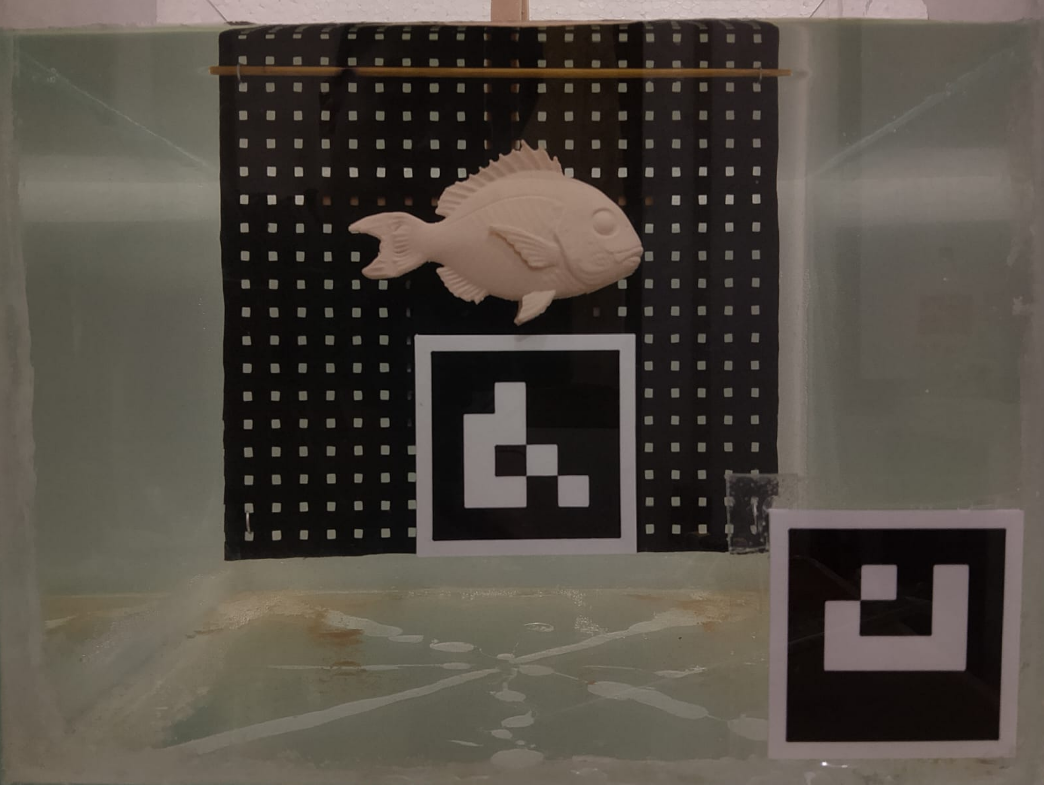
\includegraphics[width=0.75\textwidth]{fig3_2_montaje_replica.png}
\caption[Montaje de una réplica junto con el marcador ArUco coplanar]{Montaje de una réplica junto con el marcador ArUco coplanar. Fuente: elaboración propia.}
\label{fig:3-2}
\end{figure}

Para calibrar usamos un damero de $5 \times 5$ cuadros ($4 \times 4$ esquinas interiores) con cuadros de 20~mm. La calibración de B se hizo en la posición más cercana al vidrio, la de 5~cm. La separación de cada captura respecto de esa zona es la diferencia absoluta entre su distancia al vidrio y la distancia de calibración. La Figura~\ref{fig:3-3} muestra el damero y el marcador durante la preparación de la calibración.

\begin{figure}[htbp]
\centering
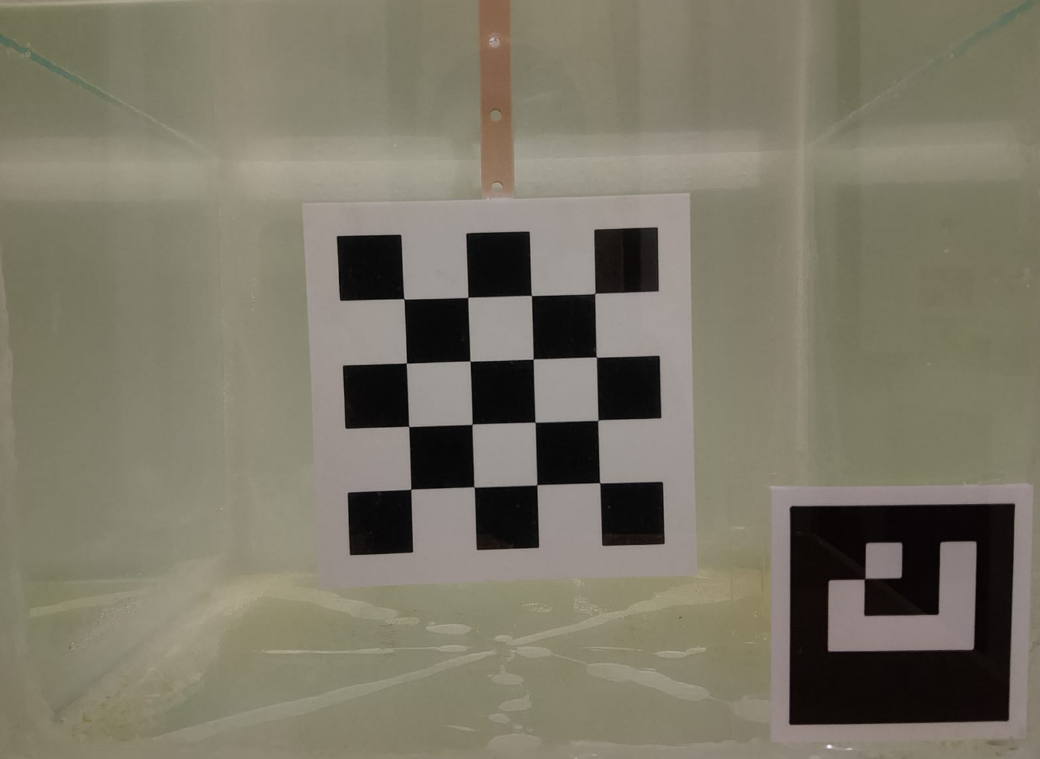
\includegraphics[width=0.75\textwidth]{fig3_3_damero.png}
\caption[Damero y marcador ArUco colocados dentro de la pecera]{Damero y marcador ArUco colocados dentro de la pecera. Fuente: elaboración propia.}
\label{fig:3-3}
\end{figure}

La Tabla~\ref{tab:puerto} reúne los parámetros físicos del puerto plano que usa C. Son, en la práctica, la ficha técnica del instrumento, y se conservan en el archivo de configuración reproducido en el Anexo~\ref{anx:flatport}.

\begin{table}[htbp]
\centering\footnotesize
\caption{Parámetros del puerto plano utilizados por la ruta C.}
\label{tab:puerto}
\begin{tabular}{@{}p{3.6cm}p{2.6cm}p{1.2cm}p{5.4cm}@{}}
\toprule
Parámetro & Valor & Unidad & Cómo se obtuvo \\
\midrule
Normal del puerto $\mathbf{n}_\pi$ & $(0, 0, 1)$ & --- & Supuesta perpendicular; comprobada con escuadra \\
Distancia cámara--vidrio $d$ & 230 & mm & Regla, desde el frente de la lente \\
Espesor del vidrio $t_g$ & 4,0 & mm & Calibre \\
Índice del aire $\mu_a$ & 1,000 & --- & Valor tabulado \\
Índice del vidrio $\mu_g$ & 1,500 & --- & Valor tabulado (vidrio \emph{float}) \\
Índice del agua $\mu_w$ & 1,333 & --- & Valor tabulado (agua dulce, 22~\si{\celsius}) \\
Condiciones del agua & 22~\si{\celsius}; salinidad 0; 0~dbar & --- & Registradas en la configuración \\
\bottomrule
\end{tabular}
\end{table}

Para ubicar el plano de medición de B observamos el damero en dos posiciones del riel (0 y 180~mm). La Tabla~\ref{tab:riel} resume los valores principales y el Anexo~\ref{anx:riel} reproduce el archivo completo. El residuo del ajuste de la dirección del riel ($1{,}62 \times 10^{-13}$~mm) es el de una recta que pasa por dos puntos: un residuo numérico, no una medida de precisión física. Los indicadores que sí informan sobre la calidad quedaron dentro de los umbrales configurados: el error de reproyección fue de 0,270~px y la dispersión de la normal, de $0{,}337^{\circ}$ (umbrales de 1,0~px y $1{,}0^{\circ}$), y el error relativo de escala, de 0,813~\%, quedó por debajo del umbral de 5~\%.

\begin{table}[htbp]
\centering\small
\caption{Referencia geométrica del riel utilizada por la ruta B.}
\label{tab:riel}
\begin{tabular}{@{}p{6cm}p{7cm}@{}}
\toprule
Campo & Valor \\
\midrule
Plano de referencia $z_{\mathrm{ref}}$ & 0,0~mm (posición nominal de 5~cm) \\
Posiciones del riel utilizadas & 0,0 y 180,0~mm \\
Error de reproyección (umbral) & 0,270~px (1,0~px) \\
Dispersión de la normal (umbral) & $0{,}337^{\circ}$ ($1{,}0^{\circ}$) \\
Error relativo de escala (umbral) & 0,813~\% (5~\%) \\
Supuesto & Planos de las réplicas paralelos al tablero \\
\bottomrule
\end{tabular}
\end{table}

\section{Software utilizado}
\label{sec:software}

Procesamos las imágenes con Fishmeter, una aplicación propia escrita en Python 3.12. El código fuente y la documentación de uso están en el repositorio público \url{\RepoURL}, etiqueta \texttt{\RepoTag}. La aplicación usa OpenCV 5.0.0 para detectar marcadores, calibrar y aplicar transformaciones geométricas; NumPy 2.5.3 para el cálculo vectorial; PyYAML 6.0.3 para los archivos de configuración; y Tkinter, de la biblioteca estándar, para la interfaz gráfica.
\\
El módulo refractivo (\texttt{refractive\_port.py} y \texttt{snells\_law.py}) implementa las ecuaciones~\eqref{eq:va} a~\eqref{eq:rayo} e incluye pruebas unitarias de sanidad. Con $\mu_g = \mu_w = 1$ y $t_g = 0$, es decir, sin vidrio ni agua, reproduce la cámara pinhole; y un rayo que viaja sobre el eje óptico no se desvía. Las pruebas de integración verifican que los cuatro métodos reciban las mismas coordenadas y que cada imagen produzca un registro trazable.

Desde la interfaz se carga la fotografía, se detectan los marcadores, se cargan o se marcan a mano los puntos anatómicos, se ejecutan los cuatro métodos y se exportan los resultados. Los clics sobre el visor se convierten a coordenadas de la imagen original antes de guardarlos o procesarlos. La Figura~\ref{fig:3-4} muestra la pantalla de marcado y comparación.

\begin{figure}[htbp]
\centering
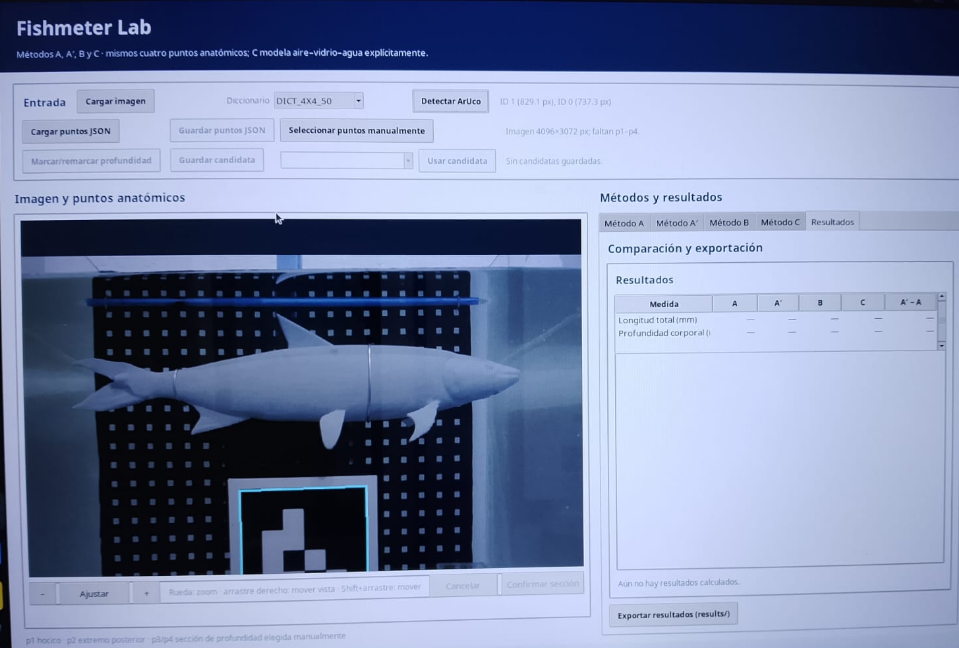
\includegraphics[width=0.8\textwidth]{fig3_4_interfaz.png}
\caption[Interfaz de Fishmeter para la marcación y comparación de métodos]{Interfaz de Fishmeter para la marcación y comparación de métodos. Fuente: Fishmeter.}
\label{fig:3-4}
\end{figure}

\section{Medidas físicas, puntos anatómicos y variables}
\label{sec:medidas}

Para cada réplica conservamos las medidas físicas de referencia de la longitud total y de la profundidad corporal (Tabla~\ref{tab:replicas}). La referencia y la imagen siguieron la misma convención anatómica, la de la Sección~\ref{sec:puntos-def}. La longitud total va desde el extremo anterior del hocico ($\mathbf{p}_1$) hasta el punto más posterior de la aleta caudal sobre el eje longitudinal ($\mathbf{p}_2$); si la cola tiene dos lóbulos, $\mathbf{p}_2$ es el extremo del lóbulo más largo. La profundidad corporal va del perfil dorsal ($\mathbf{p}_3$) al perfil ventral ($\mathbf{p}_4$) en una misma sección transversal, sin incluir las aletas.

Marcamos los cuatro puntos a mano sobre la imagen original e indicamos de forma explícita el eje longitudinal de la réplica, que usamos para proyectar las medidas. No hubo segmentación automática ni puntos distintos para cada método. La Figura~\ref{fig:3-5} resume dónde van los cuatro puntos y qué miden, y la Figura~\ref{fig:3-6} muestra los instrumentos con los que obtuvimos las dimensiones físicas de referencia.

\begin{figure}[htbp]
\centering
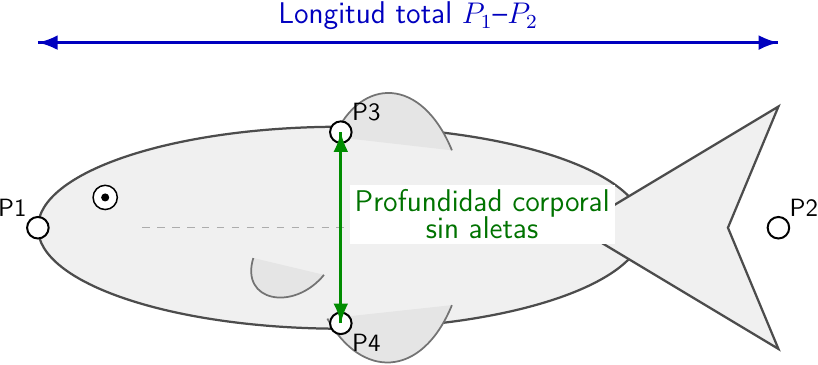
\includegraphics[width=0.7\textwidth]{fig3_5_puntos.png}
\caption[Puntos anatómicos empleados para la longitud total y la profundidad corporal]{Puntos anatómicos empleados para la longitud total y la profundidad corporal. Fuente: elaboración propia.}
\label{fig:3-5}
\end{figure}

\begin{figure}[htbp]
\centering
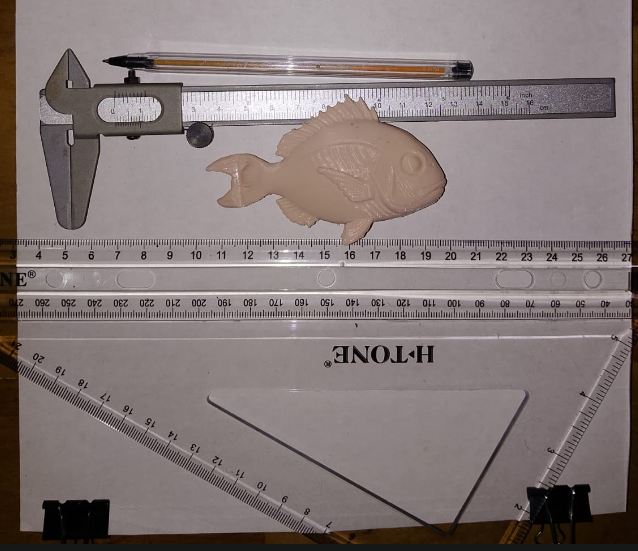
\includegraphics[width=0.6\textwidth]{fig3_6_instrumentos.png}
\caption[Instrumentos y disposición utilizados para medir físicamente una réplica]{Instrumentos y disposición utilizados para medir físicamente una réplica. Fuente: elaboración propia.}
\label{fig:3-6}
\end{figure}

Si $\mathbf{u}$ es el vector unitario del eje longitudinal y $\mathbf{n} = (-u_y, u_x)$ su normal, calculamos las medidas en el plano métrico como
\begin{equation}
\mathrm{LT} = \lvert (\mathbf{q}_2 - \mathbf{q}_1)\cdot\mathbf{u} \rvert, \qquad
\mathrm{PC} = \lvert (\mathbf{q}_4 - \mathbf{q}_3)\cdot\mathbf{n} \rvert,
\label{eq:medidas}
\end{equation}
donde $\mathbf{q}_i$ son los puntos anatómicos ya convertidos a milímetros por cada ruta. En la práctica, LT es la proyección del segmento $\mathbf{p}_1$--$\mathbf{p}_2$ sobre el eje longitudinal; si los puntos están sobre el eje, coincide con la distancia en línea recta, que es lo que mide el calibre. Una aclaración sobre los datos: en los registros del experimento, los rótulos $\mathbf{p}_1$ y $\mathbf{p}_2$ quedaron invertidos respecto de esta definición, de modo que $\mathbf{p}_1$ se marcó en el extremo caudal y $\mathbf{p}_2$ en el hocico. Como LT se calcula con el valor absoluto de la proyección (ecuación~\ref{eq:medidas}), el orden de los puntos no cambia el resultado. Solo aceptamos la profundidad corporal cuando la sección marcada era lo bastante perpendicular al eje; la aplicación guardó ese desvío como diagnóstico y permitió descartar una profundidad no válida.

La Tabla~\ref{tab:operacionalizacion} define cada variable en términos conceptuales y operacionales, y separa lo que variamos, lo que medimos y lo que mantuvimos fijo.

\begin{table}[htbp]
\centering\footnotesize
\caption{Operacionalización de las variables.}
\label{tab:operacionalizacion}
\begin{tabularx}{\textwidth}{@{}p{2.3cm} p{1.3cm} X X p{1.2cm}@{}}
\toprule
Variable & Tipo & Definición conceptual & Definición operacional & Unidad \\
\midrule
\multicolumn{5}{@{}l}{\emph{Factores variados}}\\
Método & Nominal & Ruta de conversión píxel--milímetro & A, \Aprime, B o C aplicados a los mismos puntos (Sección~\ref{sec:metodos}) & --- \\
Distancia al vidrio & Nominal & Profundidad $z$ del plano de simetría de la réplica & Posición del carrito: 5, 11, 17 o 23~cm; separación de la zona de B: 0, 6, 12 o 18~cm & cm \\
Rango de $z$ & Nominal & Conocimiento disponible sobre la profundidad & Toda la pecera (0--30~cm); $\pm 3$~cm; $\pm 1$~cm & cm \\
\multicolumn{5}{@{}l}{\emph{Resultados medidos}}\\
LT y PC estimadas & Razón & Longitud total y profundidad corporal de la réplica & Salida de Fishmeter por método, ecuación~\eqref{eq:medidas} & mm \\
LT y PC de referencia & Razón & Dimensión física de la réplica & Media de tres lecturas con calibre analógico, registradas al milímetro & mm \\
Error con signo, EA, EPA & Razón & Diferencia entre estimación y referencia & Ecuaciones~\eqref{eq:errores} & mm, mm, \% \\
Ancho relativo de $\IL$ & Razón & Extensión del intervalo por profundidad desconocida & $(\max_z L - \min_z L)/\mathrm{LT}_{\mathrm{ref}}$ & \% \\
Cobertura de $\IL$ & Razón & Fracción de capturas cuya referencia cae en $\IL$ & Conteo sobre las capturas disponibles & --- \\
\multicolumn{5}{@{}l}{\emph{Condiciones fijas}}\\
Cámara, pecera, agua, luz, marcadores, soporte, operador & --- & Condiciones del montaje & Registradas en las Secciones~\ref{sec:montaje} y~\ref{sec:procedimiento} & --- \\
\bottomrule
\end{tabularx}
\end{table}

\section{Métodos de conversión métrica}
\label{sec:metodos}

Los cuatro métodos reciben la misma imagen, los mismos cuatro puntos y el mismo eje. Lo único que cambia es la transformación que convierte píxeles en milímetros.

\begin{description}
  \item[Método A.] Usa el ArUco fijo en el vidrio. Con el lado físico $L_m$ del marcador y el promedio $\bar{p}$ de las longitudes en píxeles de sus cuatro lados (ecuación~\ref{eq:lado}), la escala implementada es
  \begin{equation}
    k = \frac{L_m}{\bar{p}}, \qquad \bar{p} = \frac{1}{4}\sum_{i=1}^{4} p_i,
    \label{eq:escala-impl}
  \end{equation}
  que difiere de la ecuación~\eqref{eq:escala-monkman} solo en el orden en que se promedia; para marcadores bien detectados, ambas coinciden hasta la tercera cifra. Cada punto se transforma como $\mathbf{q}_i = k\,\mathbf{p}_i$ y las medidas salen de la ecuación~\eqref{eq:medidas}. Es la línea de base: no corrige la diferencia de profundidad entre el vidrio y la réplica.
  \item[Método \Aprime.] Usa el ArUco montado aproximadamente en el plano de simetría de la réplica. Las cuatro esquinas del marcador en píxeles y sus coordenadas métricas $(0,0)$, $(L_m,0)$, $(L_m,L_m)$ y $(0,L_m)$ definen una homografía $\mathbf{H}$ de $3 \times 3$. Cada punto anatómico se transforma como $\tilde{\mathbf{q}}_i = \mathbf{H}\,\tilde{\mathbf{p}}_i$, en milímetros sobre el plano del marcador; el eje longitudinal se transforma igual, y las medidas salen de la ecuación~\eqref{eq:medidas}. La homografía corrige la perspectiva dentro del plano del marcador, pero no la diferencia de escala de los puntos que quedan fuera de él.
  \item[Método B.] Usa la calibración de cámara hecha con el damero sumergido y un modelo pinhole efectivo (perfil \texttt{B-effective}, Anexo~\ref{anx:calibraciones}). Los píxeles se convierten en rayos con $\mathbf{K}_{\mathrm{agua}}$ y los coeficientes de distorsión efectivos (ecuaciones~\ref{eq:pinhole} y~\ref{eq:distorsion}, invertidas), y esos rayos se intersecan con el plano $\pi_z$, paralelo al tablero de calibración y ubicado en la lectura del riel de cada captura, que ya corresponde al plano de simetría de la réplica (Tabla~\ref{tab:posiciones}). Como la calibración se fijó en la posición más cercana al vidrio, B representa de forma empírica el comportamiento óptico de esa zona. LT y PC se calculan en el espacio métrico tridimensional.
  \item[Método C.] Usa la calibración de cámara hecha en aire (perfil \texttt{C-air}) y el modelo de puerto plano de la Sección~\ref{sec:puerto-plano}. Para cada punto corregimos la distorsión de la lente, obtenemos el rayo en el aire (ecuación~\ref{eq:va}), aplicamos las dos refracciones (ecuaciones~\ref{eq:q1} a~\ref{eq:vw}) con los parámetros de la Tabla~\ref{tab:puerto} e intersecamos el rayo en el agua (ecuación~\ref{eq:rayo}) con el plano de la réplica, definido en el marco de la cámara física. Para el caso de profundidad desconocida repetimos el cálculo sobre la grilla de profundidades físicamente admisibles y lo expresamos como el intervalo geométrico de la ecuación~\eqref{eq:IL}.
\end{description}

Teníamos prevista una prueba complementaria con una barra patrón sumergida, pensada para separar un posible error de implementación del error de marcado. No la hicimos como validación separada; solo hubo una comprobación preliminar con la réplica R1 (de unos 160~mm de largo), durante las pruebas de comienzos de septiembre de 2026 (Sección~\ref{sec:delimitacion}). La validación métrica de las cuatro rutas es, entonces, la comparación directa con las longitudes y profundidades medidas con calibre en las seis réplicas y las cuatro posiciones (Capítulo~\ref{cap:resultados}). A lo largo del documento distinguimos la «comprobación instrumental con patrón» (barra sumergida, no realizada) de la «validación externa» (otras cámaras, montajes o condiciones, fuera del alcance).

\subsection{Implementación en Fishmeter}
\label{sec:implementacion}

En Fishmeter, los cuatro métodos comparten el principio y el final del cálculo. Todos parten de los mismos cuatro puntos y del mismo eje longitudinal marcados en la imagen; en todas las capturas, ese eje se indicó como la dirección horizontal de la imagen, $(1, 0)$. Todos terminan, también, en la misma operación: proyectar los segmentos $\mathbf{p}_1$--$\mathbf{p}_2$ y $\mathbf{p}_3$--$\mathbf{p}_4$ sobre los ejes anatómicos. Lo que cambia es el camino que lleva los píxeles a un espacio métrico. A y \Aprime{} llegan a un plano bidimensional en milímetros; B y C, a un plano ubicado en el espacio tridimensional de la cámara. La Tabla~\ref{tab:recorridos} resume ese camino con los nombres de las funciones del repositorio (Sección~\ref{sec:software}).

\begin{table}[htbp]
\centering\footnotesize
\caption{Recorrido de cada método en Fishmeter, desde los píxeles hasta la medición.}
\label{tab:recorridos}
\begin{tabularx}{\textwidth}{@{}p{1.1cm} >{\raggedright\arraybackslash}X >{\raggedright\arraybackslash}p{1.9cm} >{\raggedright\arraybackslash\scriptsize\ttfamily}p{5.4cm}@{}}
\toprule
Método & Conversión de los puntos & Espacio de medición & \normalfont\footnotesize Funciones principales \\
\midrule
A & Escala uniforme $k$ tomada del ArUco fijo en el vidrio & Plano 2D & measure\_a $\rightarrow$ measure\_direct $\rightarrow$ scale\_points $\rightarrow$ measure\_projected\_morphometry \\
\Aprime & Homografía $\mathbf{H}$ entre las esquinas del ArUco coplanar y un cuadrado de lado $L_m$ & Plano 2D & measure\_a\_prime $\rightarrow$ measure\_direct $\rightarrow$ marker\_plane\_homography $\rightarrow$ transform\_points\_homography $\rightarrow$ measure\_projected\_morphometry \\
B & Rayo del modelo pinhole efectivo intersecado con el plano $\pi_z$ ubicado con el riel & Plano en el espacio 3D & measure\_b $\rightarrow$ intersect\_image\_points\_with\_plane $\rightarrow$ intersect\_ray\_plane $\rightarrow$ measure\_projected\_morphometry\_3d \\
C & Rayo en aire refractado en las interfaces aire--vidrio y vidrio--agua, e intersecado con el plano de la réplica & Plano en el espacio 3D & measure\_c $\rightarrow$ \_trace\_to\_plane $\rightarrow$ trace\_refracted\_ray $\rightarrow$ intersect\_ray\_line\_plane $\rightarrow$ measure\_projected\_morphometry\_3d \\
\bottomrule
\end{tabularx}
\end{table}

\paragraph{Método A.} La función \texttt{measure\_direct} calcula el factor $k$ de la ecuación~\eqref{eq:escala-impl} y multiplica por él las coordenadas de los cuatro puntos, $\mathbf{q}_i = k\,\mathbf{p}_i$. Como una escala uniforme no cambia las direcciones, el eje marcado en la imagen sirve sin modificaciones en el plano métrico. Cada resultado de A sale con una advertencia automática: la escala viene del plano del vidrio y no corrige la separación entre planos, la perspectiva ni la refracción.

\paragraph{Método \Aprime.} La misma función calcula con OpenCV la homografía que lleva las cuatro esquinas detectadas del marcador al cuadrado métrico de lado $L_m$, y la aplica a los cuatro puntos. Una homografía no conserva las direcciones de la imagen, así que el eje se transforma como una recta: Fishmeter toma $\mathbf{p}_1$ y un segundo punto desplazado sobre el eje, transforma ambos y usa como eje métrico la dirección que los une. Lo mismo se hace en B y en C.

\paragraph{Método B.} Primero se ubica el plano de medición. El plano de referencia que guarda la calibración del riel, con un punto $\mathbf{P}_{\mathrm{ref}}$ y una normal $\mathbf{s}$, se traslada a lo largo de la dirección del riel la diferencia entre la lectura de la captura y la de calibración, $z_{\mathrm{riel}} - z_{\mathrm{ref}}$ (Tablas~\ref{tab:posiciones} y~\ref{tab:riel}); así se obtiene un punto $\mathbf{P}_0$ del plano $\pi_z$. La normal no cambia, porque suponemos que los planos de las réplicas son paralelos al tablero. Después, cada punto se corrige de distorsión con $\mathbf{K}_{\mathrm{agua}}$ y los coeficientes del perfil \texttt{B-effective}, se convierte en un rayo $\mathbf{r} = (x, y, 1)^{\mathsf{T}}$ que sale del centro de la cámara y se interseca con el plano:
\begin{equation}
\mathbf{P} = \lambda\,\mathbf{r}, \qquad \lambda = \frac{\mathbf{s}\cdot\mathbf{P}_0}{\mathbf{s}\cdot\mathbf{r}} .
\label{eq:interseccion-b}
\end{equation}
La refracción no aparece en ningún paso: queda absorbida, de forma empírica, en la calibración hecha bajo el agua.

\paragraph{Método C.} Cada punto se corrige de distorsión con la calibración en aire (perfil \texttt{C-air}) y da la dirección $\mathbf{v}_a$ de la ecuación~\eqref{eq:va}. La función \texttt{trace\_refracted\_ray} sigue ese rayo hasta la cara exterior del vidrio ($\mathbf{q}_1$), lo refracta con la ley de Snell vectorial ($\mathbf{v}_g$), lo lleva hasta la cara interior ($\mathbf{q}_2$) y lo vuelve a refractar al entrar en el agua ($\mathbf{v}_w$); son las ecuaciones~\eqref{eq:q1} a~\eqref{eq:vw}, en ese orden. En cada interfaz comprueba que el punto calculado quede sobre el plano del vidrio, con una tolerancia de $10^{-6}$~mm. El rayo en el agua (ecuación~\ref{eq:rayo}) se interseca después con el plano de la réplica, que en C es paralelo al vidrio ($\mathbf{s} = \mathbf{n}_\pi$) y contiene el punto $\mathbf{P}_0$ ubicado a $d + t_g + z$ del centro de la cámara sobre esa normal:
\begin{equation}
\mathbf{P} = \mathbf{q}_2 + \lambda\,\mathbf{v}_w, \qquad \lambda = \frac{\mathbf{s}\cdot(\mathbf{P}_0 - \mathbf{q}_2)}{\mathbf{s}\cdot\mathbf{v}_w} .
\label{eq:interseccion-c}
\end{equation}
Los dos puntos que definen el eje se trazan de la misma forma, de modo que los puntos anatómicos y el eje quedan en el mismo sistema de coordenadas.

\paragraph{Medición final.} A y \Aprime{} aplican directamente la ecuación~\eqref{eq:medidas}. En B y C, el eje transformado $\mathbf{a}$ se proyecta primero sobre el plano de medición, para quitarle cualquier componente fuera de él, y la dirección dorsoventral se obtiene con el producto vectorial:
\begin{equation}
\mathbf{u} = \frac{\mathbf{a} - (\mathbf{a}\cdot\mathbf{s})\,\mathbf{s}}{\lVert \mathbf{a} - (\mathbf{a}\cdot\mathbf{s})\,\mathbf{s} \rVert}, \qquad
\mathbf{n} = \mathbf{s} \times \mathbf{u} .
\label{eq:ejes-3d}
\end{equation}
Con esos ejes, LT y PC salen de la misma ecuación~\eqref{eq:medidas}, con los puntos tridimensionales $\mathbf{P}_i$ en lugar de $\mathbf{q}_i$. En los cuatro métodos, la profundidad corporal se valida con el ángulo de la sección,
\begin{equation}
\theta = \arctan\frac{\lvert (\mathbf{q}_4 - \mathbf{q}_3)\cdot\mathbf{u} \rvert}{\lvert (\mathbf{q}_4 - \mathbf{q}_3)\cdot\mathbf{n} \rvert},
\label{eq:angulo-seccion}
\end{equation}
que mide cuánto se aparta el segmento $\mathbf{p}_3$--$\mathbf{p}_4$ de la perpendicular al eje. Si $\theta$ supera $5^{\circ}$, Fishmeter no informa la PC y deja una advertencia; en nuestros datos ningún registro superó ese umbral. Las distancias euclidianas $\lVert \mathbf{q}_2 - \mathbf{q}_1 \rVert$ y $\lVert \mathbf{q}_4 - \mathbf{q}_3 \rVert$ se guardan con cada resultado, pero solo como diagnóstico.

\section{Procedimiento por imagen y trazabilidad}
\label{sec:procedimiento}

Las 72 imágenes siguieron exactamente la misma secuencia, la de la Figura~\ref{fig:3-flujo}:

\begin{enumerate}
  \item identificar la réplica, la distancia y la repetición, y conservar la imagen JPG original;
  \item verificar visibilidad y enfoque;
  \item marcar manualmente $\mathbf{p}_1$, $\mathbf{p}_2$, $\mathbf{p}_3$ y $\mathbf{p}_4$ en coordenadas de la imagen original;
  \item registrar el eje longitudinal y las observaciones de calidad;
  \item aplicar A, \Aprime, B y C a las mismas coordenadas;
  \item calcular LT y PC en milímetros y guardar advertencias o exclusiones;
  \item asociar cada estimación con la referencia física, la calibración, la versión del procedimiento y el nombre de la imagen.
\end{enumerate}

\begin{figure}[htbp]
\centering
\begin{tikzpicture}[>=Stealth,font=\small,node distance=4mm,
  caja/.style={draw,rounded corners=2pt,fill=gray!8,minimum height=8mm,text width=2.5cm,align=center},
  met/.style={draw,rounded corners=2pt,minimum height=7mm,text width=1.6cm,align=center,font=\small\bfseries}]
  \node[caja] (a) {Imagen JPG original};
  \node[caja,right=of a] (b) {Control de visibilidad y enfoque};
  \node[caja,right=of b] (c) {Marcado manual de $\mathbf{p}_1\ldots\mathbf{p}_4$ y eje};
  \node[caja,right=of c] (d) {Registro CSV y JSON por imagen};
  \node[met,fill=metA!15,below=9mm of b] (mA) {A};
  \node[met,fill=metAp!15,right=2mm of mA] (mAp) {\Aprime};
  \node[met,fill=metB!15,right=2mm of mAp] (mB) {B};
  \node[met,fill=metC!15,right=2mm of mB] (mC) {C};
  \node[caja,below=9mm of mAp.south east,text width=5cm] (e) {LT y PC en mm; comparación con la referencia de calibre; advertencias y exclusiones};
  \draw[->] (a) -- (b); \draw[->] (b) -- (c); \draw[->] (c) -- (d);
  \foreach \m in {mA,mAp,mB,mC}{\draw[->] (c.south) -- (\m.north); \draw[->] (\m.south) -- (e.north);}
  \draw[->] (e.east) -| (d.south);
\end{tikzpicture}
\caption[Flujo de procesamiento por imagen]{Flujo de procesamiento por imagen: los mismos cuatro puntos marcados una sola vez alimentan las cuatro rutas, y cada estimación queda asociada a su referencia física y a su registro. Fuente: elaboración propia.}
\label{fig:3-flujo}
\end{figure}

La tabla maestra guarda, para cada estimación, la réplica y la imagen, la distancia al vidrio, la repetición, el método, la medida, la referencia física, el valor estimado, el error, el estado de los puntos y del marcador, y el motivo de exclusión si lo hubo. Gracias a eso, cada número puede rastrearse hasta la fotografía original y sus coordenadas manuales. Los archivos de datos (imágenes, puntos, calibraciones y tabla maestra) y los scripts que regeneran las tablas y figuras del Capítulo~\ref{cap:resultados} están publicados (Anexo~\ref{anx:repositorio}).

\section{Evaluación de las estimaciones}
\label{sec:evaluacion}

Para cada medida calculamos el error con signo, el error absoluto y el error porcentual absoluto:
\begin{equation}
e = \hat{y} - y, \qquad \mathrm{EA} = \lvert \hat{y} - y \rvert, \qquad \mathrm{EPA} = 100\,\frac{\lvert \hat{y} - y \rvert}{y},
\label{eq:errores}
\end{equation}
donde $\hat{y}$ es la estimación del método e $y$ la referencia física. Antes de comparar métodos resumimos las tres repeticiones técnicas de cada réplica y distancia, para no tratarlas como observaciones independientes. Sobre las $n = 24$ combinaciones réplica--profundidad calculamos el sesgo, el error absoluto medio y el error porcentual absoluto medio:
\begin{equation}
\mathrm{sesgo} = \frac{1}{n}\sum_{i=1}^{n} e_i, \qquad
\mathrm{MAE} = \frac{1}{n}\sum_{i=1}^{n} \lvert e_i \rvert, \qquad
\mathrm{MAPE} = \frac{100}{n}\sum_{i=1}^{n} \frac{\lvert e_i \rvert}{y_i}.
\label{eq:agregados}
\end{equation}
Un sesgo positivo indica que el método sobreestima, y uno negativo, que subestima. Estas métricas describen la estimación promedio por condición; una captura individual puede equivocarse más, y por eso la Tabla~\ref{tab:agregados} informa también el MAE calculado captura por captura.

La comparación principal enfrenta el error de A, \Aprime, B y C en las mismas imágenes y profundidades. Las 24 combinaciones pertenecen a solo seis réplicas, es decir, son medidas repetidas; por eso hicimos la inferencia con la réplica como unidad. Para cada réplica promediamos el error absoluto de LT de las cuatro posiciones y aplicamos una prueba de signos exacta de dos colas a las diferencias pareadas entre C y cada uno de los otros métodos, y entre B y los métodos A y \Aprime{} ($n = 6$). No usamos pruebas paramétricas porque con seis réplicas no se pueden verificar sus supuestos. Los conteos sobre las 24 combinaciones réplica--profundidad se informan como descriptivos. Para ver cómo cambia el error de B y C al alejarse de la zona de calibración de B, ajustamos por mínimos cuadrados una recta a la diferencia de MAE frente a la separación y usamos su pendiente.

Con C calculamos además el intervalo de longitudes que resulta de recorrer todas las profundidades admisibles. Ese intervalo expresa incertidumbre geométrica por profundidad; no es un intervalo de confianza estadístico. Evaluamos su ancho relativo en tres escenarios de conocimiento de $z$ (toda la pecera, $\pm 3$~cm y $\pm 1$~cm) y lo comparamos con la predicción de primer orden de la ecuación~\eqref{eq:Dz}. Para eso corrimos C en cada captura con el plano de medición en $z = 0, 10, \ldots, 300$~mm, y calculamos la cobertura empírica como la fracción de las 72 capturas cuya LT de calibre cayó dentro de $\IL$. Describimos también la concordancia de B y C con la referencia mediante el sesgo y los límites de acuerdo de Bland--Altman \parencite{Bland1986}, calculados como el sesgo $\pm 1{,}96$ veces la desviación estándar de las diferencias sobre las 24 combinaciones (Sección~\ref{sec:discusion}).

\section{Alcance y limitaciones metodológicas}
\label{sec:limitaciones-metod}

El procedimiento mide réplicas rígidas y ubica los puntos a mano; no es un sistema de segmentación automática ni una medición completamente automática. Medimos la distancia cámara--vidrio desde el frente de la lente y tomamos los índices de refracción de tablas; la Sección~\ref{sec:sensibilidad} cuantifica cuánto afectan estos dos parámetros a C. La exactitud de B depende de que el plano de medición se exprese en el marco de su calibración, a través de la referencia del riel (Tablas~\ref{tab:posiciones} y~\ref{tab:riel}). No hicimos la comprobación instrumental con barra patrón sumergida; la validación métrica del trabajo es la comparación con las referencias de calibre de las réplicas.

\section{Cuestiones éticas y uso de herramientas}
\label{sec:etica}

No usamos animales ni datos de terceros: las réplicas, las imágenes, las calibraciones y las medidas son propias. El autor desarrolló el código de la aplicación, incluido el módulo refractivo, y su historial de versiones está en el repositorio. Durante la redacción se usaron herramientas de asistencia basadas en modelos de lenguaje para revisar la estructura del documento, la consistencia de la notación y el estilo, y para preparar borradores de secciones a partir de los datos del autor. El diseño experimental, la captura, el marcado, el análisis y las conclusiones son responsabilidad del autor, que revisó y validó todo el texto.

\chapter{Resultados y discusión}
\label{cap:resultados}

Este capítulo presenta los resultados registrados en el CSV maestro del experimento. El análisis se realizó sobre el experimento principal, conservando la correspondencia entre cada imagen, la réplica, la profundidad, la repetición técnica y el método de conversión métrica. Las cifras se informan como una comparación dentro del montaje utilizado y contra las referencias físicas de las réplicas; no se interpretan como una validación del sistema en otras condiciones.

\section{Composición del conjunto y control de calidad}
\label{sec:conjunto}

El archivo contiene 288 registros: 72 imágenes, seis réplicas de PLA, cuatro posiciones nominales respecto del vidrio (5, 11, 17 y 23~cm), tres capturas técnicas por condición y cuatro métodos (A, \Aprime, B y C). Por cada combinación de réplica y profundidad se dispone, en general, de tres capturas. Las capturas repetidas se trataron como repeticiones técnicas y no como réplicas independientes.

Se obtuvieron valores numéricos para 284 registros. Los cuatro registros sin medición corresponden a A y \Aprime{} en dos imágenes en las que no se detectó el marcador ArUco: \texttt{R2-REP2-170.jpg} y \texttt{R3-REP2-50.jpg}. El motivo se conservó en el CSV y esos registros se excluyeron de los cálculos de error. Los métodos B y C produjeron valores para las 72 imágenes. La aplicación conserva para ambos un estado interno \texttt{PENDING\_VALIDATION}, que solo cambia cuando se registra una barra patrón sumergida; esa comprobación instrumental complementaria no se realizó (Sección~\ref{sec:metodos}). La validación métrica de B y C en este trabajo es la comparación directa con las longitudes y profundidades de calibre de las seis réplicas en las cuatro posiciones, que se presenta en las Secciones~\ref{sec:agregados} y~\ref{sec:profundidad}. La Tabla~\ref{tab:registros} resume el tratamiento de los registros.

\begin{table}[htbp]
\centering\small
\caption{Registros del CSV y su tratamiento en el análisis.}
\label{tab:registros}
\begin{tabular}{@{}lccp{7.5cm}@{}}
\toprule
Método & Registros & Con valor & Tratamiento \\
\midrule
A & 72 & 70 & Se excluyeron dos registros por falta de detección del ArUco. \\
\Aprime & 72 & 70 & Se excluyeron dos registros por falta de detección del ArUco. \\
B & 72 & 72 & Valor numérico en las 72 imágenes; evaluado contra la referencia de calibre. \\
C & 72 & 72 & Valor numérico en las 72 imágenes; evaluado contra la referencia de calibre. \\
\bottomrule
\end{tabular}
\end{table}

En las dos combinaciones afectadas por la ausencia de ArUco, A y \Aprime{} se promediaron con las dos capturas disponibles, mientras que B y C usaron las tres; el pareamiento no es por ello idéntico en esas dos combinaciones. Al repetir el cálculo de las Tablas~\ref{tab:agregados} y~\ref{tab:posiciones-mae} solo con las 70 imágenes comunes a los cuatro métodos, ningún valor cambió en más de 0,01~mm o 0,01 puntos porcentuales, y los conteos de la comparación pareada de la Sección~\ref{sec:agregados} se mantuvieron; los resultados no dependen de esas dos capturas.

\section{Calibraciones}
\label{sec:calibraciones}

Las dos calibraciones de cámara se realizaron el 12 de octubre de 2026 con el damero de $4 \times 4$ esquinas interiores y cuadros de 20~mm, a la resolución de captura de $4096 \times 3072$ píxeles. La Tabla~\ref{tab:calibraciones} resume sus indicadores de calidad; los perfiles completos se reproducen en el Anexo~\ref{anx:calibraciones}.

\begin{table}[htbp]
\centering\footnotesize
\caption{Calibraciones de cámara utilizadas por las rutas B y C.}
\label{tab:calibraciones}
\begin{tabular}{@{}p{4.2cm}p{4.4cm}p{4.4cm}@{}}
\toprule
Campo & Perfil B (bajo agua) & Perfil C (en aire) \\
\midrule
Identificador & \texttt{B-effective} & \texttt{C-air} \\
Rutina & \texttt{calibrateCamera} (OpenCV 5.0.0) & \texttt{calibrateCamera} (OpenCV 5.0.0) \\
RMS de reproyección & 0,4354~px & 0,3745~px \\
Vistas recibidas / aceptadas & 35 / 35 & 36 / 36 \\
Vistas rechazadas & 0 & 0 \\
Focal efectiva $f_x$ & 4502,3~px & 3313,7~px \\
Punto principal $(c_x, c_y)$ & (2027,3; 1549,0)~px & (2028,2; 1530,6)~px \\
\bottomrule
\end{tabular}
\end{table}

Ambos valores de RMS están por debajo de 0,5~px, umbral habitual para una calibración aceptable, y ninguna vista fue rechazada. La razón entre las focales efectivas, $f_{x,\mathrm{agua}}/f_{x,\mathrm{aire}} = 4502{,}3/3313{,}7 = 1{,}36$, es consistente con el índice de refracción del agua ($\mu_w = 1{,}333$): la calibración de B absorbe la refracción en una focal efectiva mayor. Para incidencia cercana a la normal, un puerto plano equivale en primer orden a una cámara pinhole con la focal multiplicada por $\mu_w$ y el centro de proyección desplazado, de modo que el modelo efectivo puede reproducir la escala a distintas profundidades si el plano de medición se ubica correctamente; los efectos no centrales que lo hacen depender de la distancia crecen con el ángulo de incidencia \parencite{Rofallski2022}.

\subsection{Sensibilidad de C a los parámetros del montaje}
\label{sec:sensibilidad}

\begin{table}[htbp]
\centering\footnotesize
\caption{Sensibilidad de la longitud total estimada por C a los parámetros medidos a mano: cambio medio con signo sobre las 72 capturas respecto de la configuración base ($d = 230$~mm, $\mu_w = 1{,}333$).}
\label{tab:sensibilidad}
\begin{tabular}{@{}p{4cm}p{2.6cm}p{2.8cm}p{2.8cm}@{}}
\toprule
Parámetro & Variación & Cambio medio de LT (mm) & Cambio medio de LT (\%) \\
\midrule
Distancia cámara--vidrio $d$ & $-20$~\% (184~mm) & $-20{,}57$ & $-14{,}01$ \\
Distancia cámara--vidrio $d$ & $+20$~\% (276~mm) & $+20{,}57$ & $+14{,}01$ \\
Índice del agua $\mu_w$ & $-0{,}01$ (1,323) & $+0{,}34$ & $+0{,}23$ \\
Índice del agua $\mu_w$ & $+0{,}01$ (1,343) & $-0{,}33$ & $-0{,}23$ \\
\bottomrule
\end{tabular}
\end{table}

C se recalculó sobre las 72 capturas con cada variante, conservando la distancia $z$ de la réplica a la cara interna del vidrio; al cambiar $d$ se desplazaron tanto la interfaz como el plano de medición. Un error de $\pm 20$~\% en $d$ ($\pm 46$~mm) cambió la LT en 20,57~mm (14,01~\%) en promedio, en concordancia con la aproximación de primer orden de la ecuación~\eqref{eq:Dz}, según la cual una variación $\Delta d$ cambia la longitud estimada en una fracción $\Delta d / D(z)$, con $D(z)$ entre 270 y 405~mm en las posiciones estudiadas. Esto equivale a cerca de 0,3~\% de LT por milímetro de error en $d$: un error de 5~mm ya supera el MAPE de C (0,88~\%). La distancia cámara--vidrio es, por tanto, el parámetro del montaje que más condiciona la exactitud de C y debe medirse con cuidado. En cambio, una variación de $\pm 0{,}01$ en $\mu_w$ cambió la LT en 0,34~mm (0,23~\%) en promedio y en no más de 0,70~mm en una captura individual, por debajo del MAE de C, de modo que el uso de un índice tabulado no limitó la exactitud.

\section{Resultados agregados por método}
\label{sec:agregados}

Las métricas se calcularon según la Sección~\ref{sec:evaluacion} después de promediar las tres capturas de cada combinación réplica--profundidad, de modo que la comparación principal quedó formada por 24 combinaciones por método. La Tabla~\ref{tab:agregados} resume las diferencias entre las estimaciones promediadas y sus referencias físicas, y la Figura~\ref{fig:4-1} las presenta gráficamente. A presenta sesgo negativo en ambas medidas, mientras que \Aprime{} y C tienden a sobreestimar; B tiene un sesgo prácticamente nulo en LT ($+0{,}05$~mm) y levemente negativo en PC ($-0{,}32$~mm). B y C obtienen los menores errores, con valores cercanos entre sí; \Aprime{} queda en tercer lugar y A es el método más afectado.

\begin{table}[htbp]
\centering\footnotesize
\caption{Errores medios por método después de resumir las repeticiones técnicas.}
\label{tab:agregados}
\begin{tabular}{@{}lccccccccc@{}}
\toprule
 & & \multicolumn{6}{c}{Promedio por combinación} & \multicolumn{2}{c}{Por captura} \\
\cmidrule(lr){3-8}\cmidrule(l){9-10}
Método & $n$ & Sesgo LT & MAE LT & MAPE LT & Sesgo PC & MAE PC & MAPE PC & MAE LT & MAE PC \\
 & & (mm) & (mm) & (\%) & (mm) & (mm) & (\%) & (mm) & (mm) \\
\midrule
A       & 24 & $-37{,}43$ & 37,43 & 25,68 & $-9{,}07$ & 9,07 & 25,25 & 37,75 & 9,16 \\
\Aprime & 24 & $+3{,}29$  & 3,29  & 2,28  & $+0{,}95$ & 1,03 & 2,78 & 3,33 & 1,03 \\
B       & 24 & $+0{,}05$  & 1,08  & 0,73  & $-0{,}32$ & 0,38 & 1,26 & 1,35 & 0,54 \\
C       & 24 & $+1{,}07$  & 1,22  & 0,88  & $+0{,}29$ & 0,56 & 1,62 & 1,34 & 0,58 \\
\bottomrule
\end{tabular}

\smallskip
\begin{minipage}{0.9\textwidth}\footnotesize
\emph{Nota.} $n$ es el número de combinaciones réplica--profundidad, no el número de fotografías. Las métricas promediadas describen la estimación promedio por condición. Las dos últimas columnas se calcularon sobre las capturas individuales: 70 para A y \Aprime{} y 72 para B y C.
\end{minipage}
\end{table}

\begin{figure}[htbp]
\centering
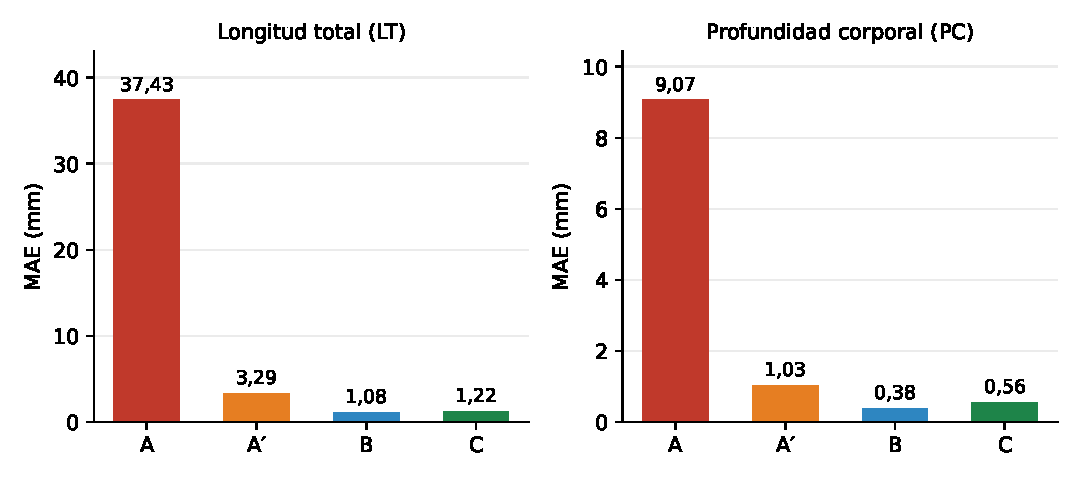
\includegraphics[width=\textwidth]{fig4_1_mae_por_metodo.pdf}
\caption[MAE por método para longitud total y profundidad corporal]{Error absoluto medio por método para longitud total (izquierda) y profundidad corporal (derecha), sobre las 24 combinaciones réplica--profundidad (datos de la Tabla~\ref{tab:agregados}). Fuente: elaboración propia.}
\label{fig:4-1}
\end{figure}

En LT, A subestimó en promedio 37,43~mm. La homografía de \Aprime{} redujo el MAE a 3,29~mm, y las dos rutas que usan la profundidad conocida con un modelo de cámara calibrado lo llevaron a 1,08~mm (B) y 1,22~mm (C). En PC se observó el mismo orden: A alcanzó un MAE de 9,07~mm, \Aprime{} de 1,03~mm, C de 0,56~mm y B de 0,38~mm. Calculado sobre las capturas individuales, el MAE de LT de B y C fue prácticamente igual (1,35 y 1,34~mm).

En la comparación pareada de LT, C tuvo menor error absoluto que A y que \Aprime{} en las 24 combinaciones, y B fue mejor que A en las 24 y que \Aprime{} en 23 (la excepción fue R2 a 5~cm). Con la réplica como unidad experimental, tanto B como C tuvieron menor error absoluto medio de LT que A y que \Aprime{} en las seis réplicas; la prueba de signos exacta de dos colas sobre las seis diferencias pareadas da $p = 2/2^{6} = 0{,}031$ en cada una de esas cuatro comparaciones. Entre B y C no hubo diferencia: C tuvo menor error de LT en 10 de las 24 combinaciones y en 3 de las 6 réplicas (R2, R5 y R6; $p = 1$). Los conteos sobre las 24 combinaciones se reportan como descriptivos porque las combinaciones de una misma réplica no son independientes. Para PC, C fue mejor que A en las 24 combinaciones y que \Aprime{} en 21 (5 de 6 réplicas, $p = 0{,}219$; la excepción fue R5, con un MAE de PC de 0,32~mm para \Aprime{} y 0,75~mm para C), y B fue mejor que C en 16 de las 24 combinaciones y en 5 de las 6 réplicas ($p = 0{,}219$), de nuevo con R5 como excepción.

\section{Comportamiento según la profundidad}
\label{sec:profundidad}

La dependencia con la distancia al vidrio se aprecia con mayor claridad en la longitud total. La Tabla~\ref{tab:posiciones-mae} presenta el MAE de LT para cada posición, calculado después de promediar las repeticiones técnicas, y la Figura~\ref{fig:4-2} muestra las cuatro curvas.

\begin{table}[htbp]
\centering\footnotesize
\caption{MAE de longitud total (mm) por posición de la réplica.}
\label{tab:posiciones-mae}
\begin{tabular}{@{}p{1.6cm}p{2.6cm}ccccc@{}}
\toprule
Distancia (cm) & Separación de la zona de B (cm) & A & \Aprime & B & C & B $-$ C \\
\midrule
5  & 0  & 13,77 & 3,44 & 1,18 & 1,09 & $+0{,}09$ \\
11 & 6  & 32,02 & 3,18 & 1,10 & 1,41 & $-0{,}31$ \\
17 & 12 & 46,29 & 3,44 & 1,01 & 1,29 & $-0{,}28$ \\
23 & 18 & 57,64 & 3,11 & 1,04 & 1,07 & $-0{,}04$ \\
\bottomrule
\end{tabular}
\end{table}

\begin{figure}[htbp]
\centering
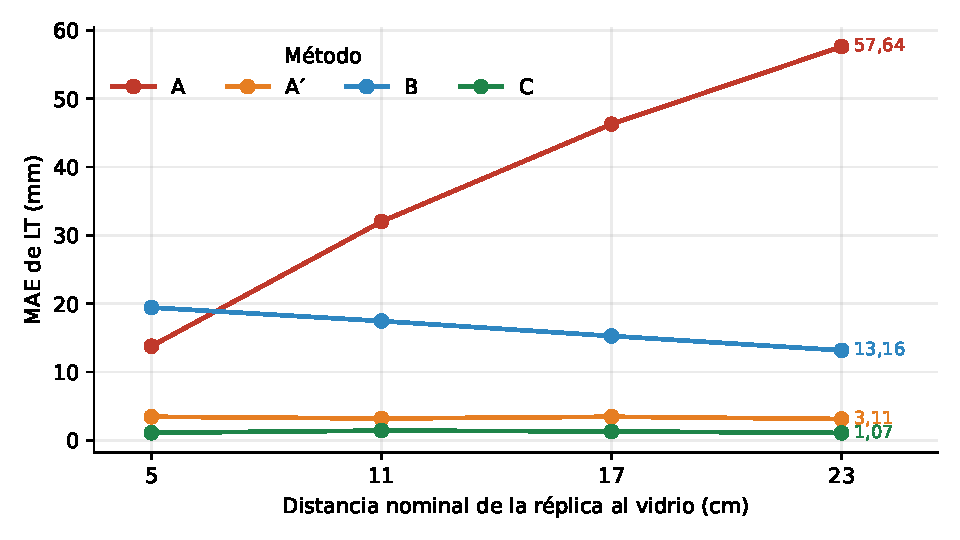
\includegraphics[width=0.9\textwidth]{fig4_2_mae_lt_profundidad.pdf}
\caption[MAE de longitud total por método y profundidad]{Error absoluto medio de longitud total por método y distancia de la réplica al vidrio (datos de la Tabla~\ref{tab:posiciones-mae}). El error de A crece con la profundidad; \Aprime, B y C se mantienen estables, y las curvas de B y C casi se superponen. Fuente: elaboración propia.}
\label{fig:4-2}
\end{figure}

El error de A aumentó de 13,77~mm a 5~cm hasta 57,64~mm a 23~cm, con una pendiente de 2,43~mm por centímetro de separación. Este comportamiento es compatible con una escala calculada en el plano del vidrio: al alejarse la réplica, la misma escala deja de representar adecuadamente su plano de medición. La predicción de primer orden de la ecuación~\eqref{eq:Dz} para una réplica de 140~mm da errores de $-19$, $-37$, $-50$ y $-60$~mm en las cuatro posiciones, frente a los $-14$, $-32$, $-46$ y $-58$~mm observados; la diferencia máxima, de 6~mm, es atribuible a que $d$ se midió desde el frente de la lente y a que las réplicas tienen longitudes distintas. Esta coincidencia es una verificación independiente del modelo óptico: el error de A es el que la geometría predice.

\Aprime{} se mantuvo cerca de 3,1--3,5~mm en todas las posiciones, lo que indica que el marcador coplanar redujo la variación asociada a la perspectiva. B permaneció entre 1,01 y 1,18~mm y C entre 1,07 y 1,41~mm, sin tendencia con la profundidad. La diferencia B $-$ C osciló entre $-0{,}31$ y $+0{,}09$~mm, con una pendiente de $-0{,}006$~mm por centímetro de separación: el error de B no aumentó al alejarse la réplica de la zona de calibración.

Para PC se observó un patrón equivalente para A: el MAE pasó de 3,02~mm a 5~cm a 14,24~mm a 23~cm. \Aprime{} varió entre 0,75 y 1,34~mm, B entre 0,25 y 0,48~mm y C entre 0,48 y 0,62~mm.

La Figura~\ref{fig:4-errores} muestra el error con signo de cada combinación réplica--profundidad, además de su media por posición. La dispersión de A crece con la profundidad junto con su sesgo; en LT, la de \Aprime{} fue de 4 a 5~mm alrededor de un sesgo positivo, y la de B y C fue similar entre sí, de 3,4 a 4,8~mm. Esa dispersión se repite entre posiciones para una misma réplica: R4 tuvo el mayor error absoluto de LT en \Aprime, B y C en las cuatro posiciones (en B y C, entre $+2{,}1$ y $+4{,}3$~mm), y su referencia de LT es una de las dos con mayor desviación entre lecturas (2,9~mm; Tabla~\ref{tab:replicas}). Esto apunta a la referencia de calibre o al marcado de esa réplica más que a la conversión.

\begin{figure}[htbp]
\centering
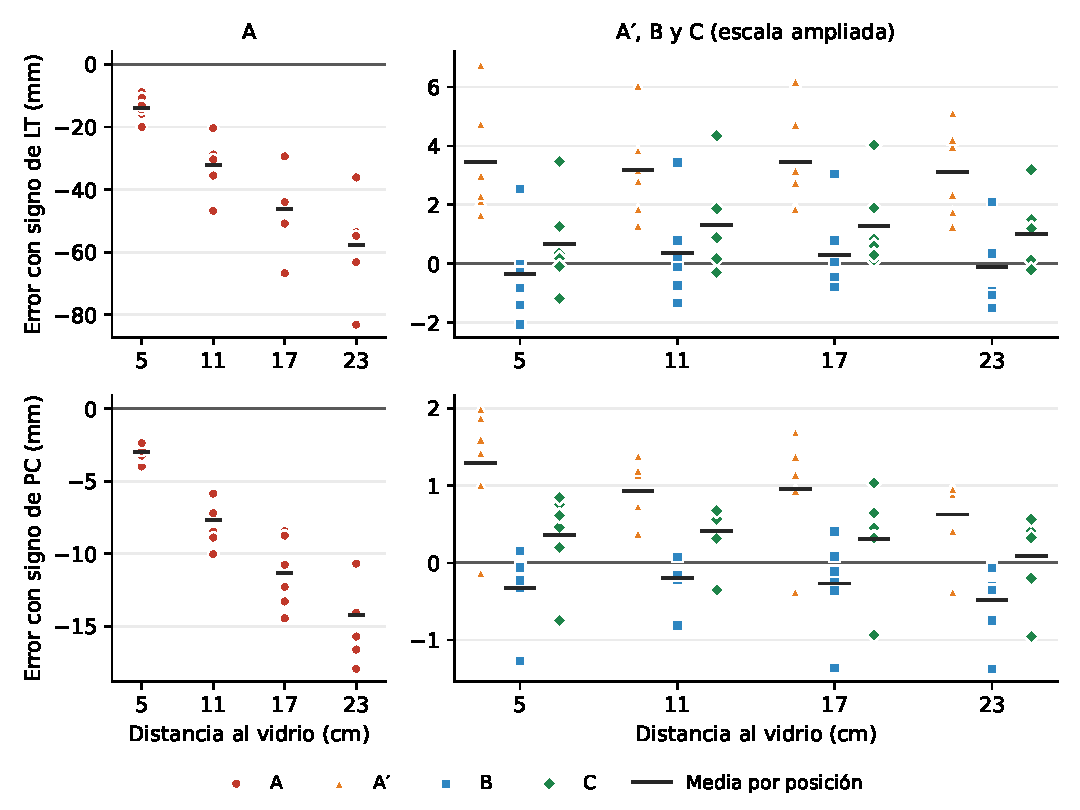
\includegraphics[width=\textwidth]{fig4_errores_combinaciones.pdf}
\caption[Error con signo por combinación réplica--profundidad]{Error con signo de LT (arriba) y PC (abajo) para cada una de las 24 combinaciones réplica--profundidad, después de promediar las repeticiones técnicas. A se presenta en un panel propio por su escala; \Aprime, B y C comparten un eje ampliado. Cada punto es una réplica y la línea horizontal, la media por posición. Fuente: elaboración propia.}
\label{fig:4-errores}
\end{figure}

\section{Repetibilidad del marcado manual}
\label{sec:repetibilidad}

\pendiente{Volver a marcar los cuatro puntos en doce imágenes (una por réplica a 5 y a 23~cm) sin consultar el marcado anterior, y completar la Tabla~\ref{tab:repetibilidad} con la diferencia media y máxima en píxeles por punto y su efecto en milímetros sobre LT y PC calculado con C. Cerrar con: «La repetibilidad del marcado introduce una variación de X~mm en LT, inferior/comparable al MAE de C y muy inferior a la diferencia entre métodos, por lo que las conclusiones de las Secciones~\ref{sec:agregados} y~\ref{sec:profundidad} no dependen del operador».}

\begin{table}[htbp]
\centering\footnotesize
\caption{Repetibilidad del marcado manual sobre doce imágenes remarcadas.}
\label{tab:repetibilidad}
\begin{tabular}{@{}p{3cm}p{2cm}p{2.2cm}p{3.2cm}p{1.6cm}@{}}
\toprule
Punto & Diferencia media (px) & Diferencia máxima (px) & Efecto medio en la medida (mm, con C) & Medida afectada \\
\midrule
$\mathbf{p}_1$ (hocico) & \pend{ } & \pend{ } & \pend{ } & LT \\
$\mathbf{p}_2$ (extremo caudal) & \pend{ } & \pend{ } & \pend{ } & LT \\
$\mathbf{p}_3$ (perfil dorsal) & \pend{ } & \pend{ } & \pend{ } & PC \\
$\mathbf{p}_4$ (perfil ventral) & \pend{ } & \pend{ } & \pend{ } & PC \\
\bottomrule
\end{tabular}
\end{table}

\section{Intervalo por profundidad desconocida}
\label{sec:intervalo}

La pregunta principal de este trabajo es qué intervalo de longitud puede garantizar C cuando la profundidad $z$ es desconocida y en qué condiciones ese intervalo es utilizable. Con el modelo de puerto plano, la longitud estimada para una misma imagen es una función $L(z)$ de la profundidad asumida; el intervalo $\IL$ de la ecuación~\eqref{eq:IL} recoge su variación sobre el rango admisible.

Para incidencia cercana a la normal, la magnificación de un punto situado a profundidad $z$ detrás del vidrio es, en primer orden, proporcional a $1/D(z)$, con $D(z) = d + t_g/\mu_g + z/\mu_w$ (ecuación~\ref{eq:Dz}), donde $d = 230$~mm, $t_g = 4$~mm, $\mu_g = 1{,}5$ y $\mu_w = 1{,}333$. Por tanto, $L(z)$ es proporcional a $D(z)$, creciente en $z$, y el intervalo puede escribirse como $[L(z_{\min}), L(z_{\max})]$. Esta misma relación reproduce el error observado de A dentro de 6~mm (Sección~\ref{sec:profundidad}), lo que respalda su uso para el intervalo.

Con ella, el ancho relativo de $\IL$ para una réplica situada a profundidad real $z_0$ es $(D(z_{\max}) - D(z_{\min}))/D(z_0)$. Para verificar esa predicción, C se ejecutó sobre las 72 capturas con el plano de medición en $z = 0, 10, 20, \ldots, 300$~mm. $L(z)$ resultó estrictamente creciente en las 72 capturas (Figura~\ref{fig:4-Lz}), lo que confirma que $\IL = [L(z_{\min}), L(z_{\max})]$. La Tabla~\ref{tab:intervalo} y la Figura~\ref{fig:4-3} presentan el ancho numérico, expresado como porcentaje de la LT de calibre, para las cuatro posiciones y tres escenarios de conocimiento de $z$: desconocida en toda la pecera (0--30~cm), conocida con $\pm 3$~cm y conocida con $\pm 1$~cm. La predicción de primer orden, que se indica entre paréntesis, difirió del cálculo numérico en 0,6~\% en promedio.

\begin{table}[htbp]
\centering\footnotesize
\caption{Ancho relativo del intervalo $\IL$ (\% de la LT de calibre) según la profundidad de la réplica y el conocimiento disponible sobre $z$: cálculo numérico con C sobre las 72 capturas y, entre paréntesis, predicción geométrica de primer orden. La última columna indica la cobertura empírica.}
\label{tab:intervalo}
\begin{tabular}{@{}lccccc@{}}
\toprule
Conocimiento de $z$ & 5~cm & 11~cm & 17~cm & 23~cm & Cobertura \\
\midrule
Desconocida (0--30~cm) & 81,8 (83,3) & 71,0 (71,4) & 62,4 (62,5) & 55,6 (55,5) & 1,00 \\
Conocida con $\pm 3$~cm & 16,4 (16,7) & 14,2 (14,3) & 12,5 (12,5) & 11,1 (11,1) & 1,00 \\
Conocida con $\pm 1$~cm & 5,5 (5,6) & 4,7 (4,8) & 4,2 (4,2) & 3,7 (3,7) & 0,81 \\
\midrule
MAPE de \Aprime{} ($z$ conocida) & \multicolumn{4}{c}{2,3} & \\
MAPE de B ($z$ conocida) & \multicolumn{4}{c}{0,7} & \\
MAPE de C ($z$ conocida) & \multicolumn{4}{c}{0,9} & \\
\bottomrule
\end{tabular}
\end{table}

\begin{figure}[htbp]
\centering
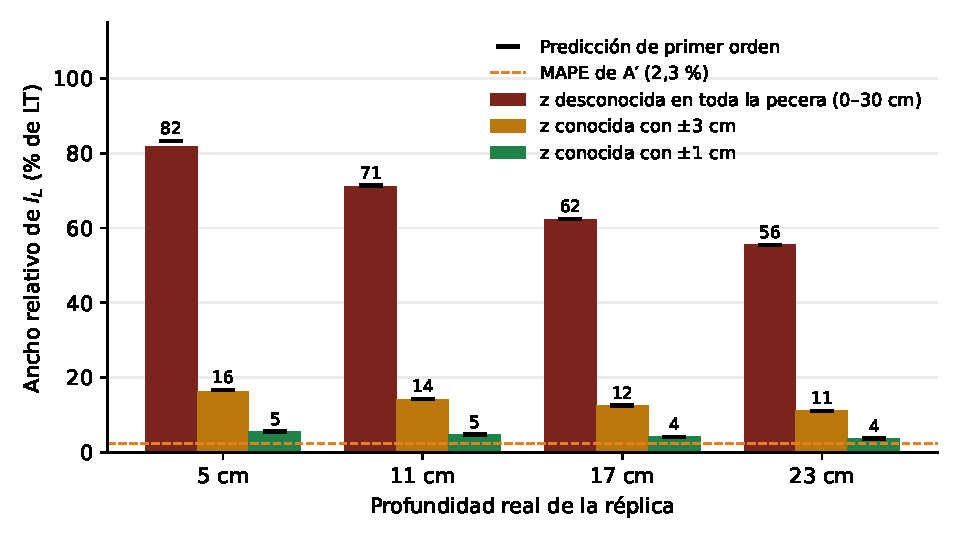
\includegraphics[width=0.9\textwidth]{fig4_3_ancho_intervalo.pdf}
\caption[Ancho relativo del intervalo por profundidad desconocida]{Ancho relativo del intervalo $\IL$ según la profundidad real de la réplica y el conocimiento disponible sobre $z$ (datos de la Tabla~\ref{tab:intervalo}). Las barras muestran el cálculo numérico y los marcadores negros la predicción de primer orden; la línea discontinua marca el MAPE de \Aprime{} con profundidad conocida. Fuente: elaboración propia.}
\label{fig:4-3}
\end{figure}

Con una sola cámara y sin información de profundidad, el intervalo abarca entre 56 y 82~\% de la longitud de la réplica: no es utilizable para morfometría. Si la profundidad se acota a $\pm 3$~cm (por ejemplo, con una guía o un tanque angosto), el ancho baja a 11--16~\%, todavía mayor que el error de \Aprime, B y C con $z$ conocida. Solo cuando la profundidad se conoce con $\pm 1$~cm el ancho (4--5~\%) se vuelve comparable con el error de \Aprime{} (2,3~\%) y queda dentro de un orden de magnitud del de B y C (0,7 y 0,9~\%). La cobertura empírica fue completa (72 de 72 capturas) en toda la pecera y con $\pm 3$~cm, pero bajó a 0,81 (58 de 72) con $\pm 1$~cm: con una ventana tan estrecha, el propio error de C con $z$ conocida basta para que la LT de calibre quede fuera del intervalo en algunas capturas. Este es el resultado que responde la pregunta principal: el modelo refractivo elimina el error de conversión, pero la profundidad sigue siendo la fuente dominante de incertidumbre y debe medirse o acotarse, no asumirse.

\begin{figure}[htbp]
\centering
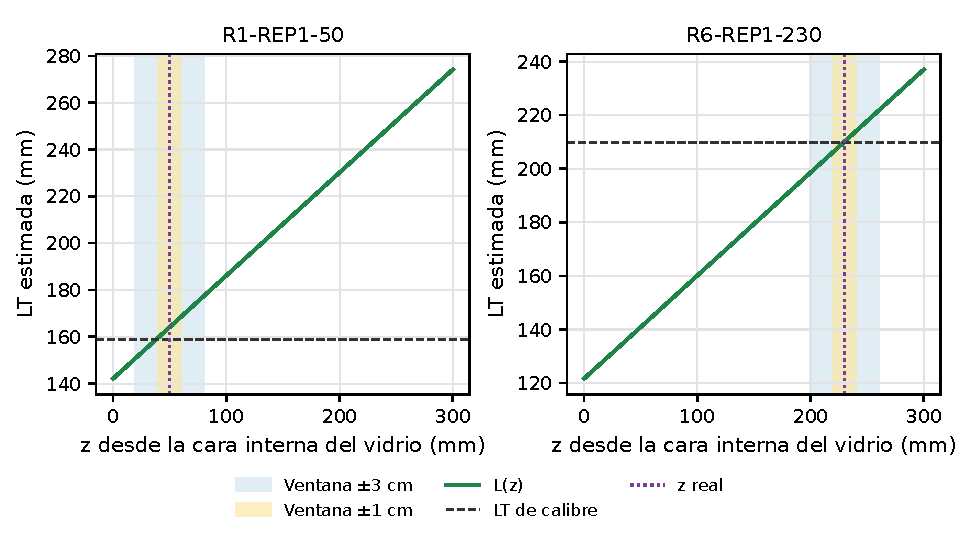
\includegraphics[width=0.9\textwidth]{fig4_L_z_ejemplos.pdf}
\caption[Longitud estimada por C en función de la profundidad supuesta]{Longitud total estimada por C en función de la profundidad supuesta $z$ para dos capturas (R1-REP1 a 5~cm y R6-REP1 a 23~cm). La línea discontinua horizontal indica la LT de calibre, la línea punteada vertical la profundidad nominal y las bandas las ventanas de $\pm 1$ y $\pm 3$~cm. Fuente: elaboración propia.}
\label{fig:4-Lz}
\end{figure}

\section{Contraste de hipótesis}
\label{sec:contraste}

La Tabla~\ref{tab:hipotesis} resume el contraste de las tres hipótesis con los criterios fijados en la Sección~\ref{sec:evaluacion}.

\begin{table}[htbp]
\centering\small
\caption{Contraste de hipótesis.}
\label{tab:hipotesis}
\begin{tabularx}{\textwidth}{@{}p{1.2cm} X X p{2.3cm}@{}}
\toprule
Hipótesis & Criterio & Valor observado & Veredicto \\
\midrule
H1 & Prueba de signos exacta por réplica, $p < 0{,}05$, para C frente a A, \Aprime{} y B en LT & Frente a A y \Aprime: C mejor en 6 de 6 réplicas ($p = 0{,}031$) y en 24 de 24 combinaciones. Frente a B: C mejor en 3 de 6 réplicas ($p = 1$) y en 10 de 24 combinaciones & Se sostiene frente a A y \Aprime; no frente a B \\
H2 & Pendiente positiva de $\mathrm{MAE}_B - \mathrm{MAE}_C$ frente a la separación & Pendiente $-0{,}006$~mm/cm ($+0{,}09$; $-0{,}31$; $-0{,}28$; $-0{,}04$~mm) & No se sostiene \\
H3 & Cobertura $\geq 0{,}95$ y ancho predicho dentro de la mitad del observado & Cobertura 1,00 (72 de 72) en toda la pecera; ancho numérico 56--82~\%, razón predicho/numérico 1,006 & Se sostiene \\
\bottomrule
\end{tabularx}
\end{table}

\paragraph{H1 se sostiene parcialmente.} C tuvo menor error absoluto de LT que A y \Aprime{} en las seis réplicas (prueba de signos exacta con la réplica como unidad, $p = 0{,}031$ en cada comparación) y en las 24 combinaciones réplica--profundidad (descriptivo), pero no que B: cada ruta fue mejor en tres réplicas ($p = 1$) y C lo fue en 10 de las 24 combinaciones. En PC, C fue mejor que A en 24 de 24 combinaciones y que \Aprime{} en 21 de 24, mientras que B fue mejor que C en 16 de 24. La parte de H1 que, en el protocolo, preveía equivalencia entre B y C dentro de la zona de calibración no se evaluó formalmente porque el margen $\delta$ no se fijó antes de observar los datos; a 5~cm el MAE de LT fue de 1,18~mm (B) y 1,09~mm (C), una diferencia de 0,09~mm, menor que la desviación de las referencias de calibre (Tabla~\ref{tab:replicas}) y compatible con que ambas rutas sean intercambiables en esa zona.

\paragraph{H2 no se sostiene.} La diferencia B $-$ C no aumentó con la separación ($+0{,}09$; $-0{,}31$; $-0{,}28$ y $-0{,}04$~mm; pendiente $-0{,}006$~mm/cm), y el MAE de B se mantuvo entre 1,01 y 1,18~mm en las cuatro posiciones. Hasta 18~cm de separación de la zona de calibración, la degradación con la distancia descrita por \textcite{Rofallski2022} no fue detectable con la resolución de este experimento; la interpretación se desarrolla en la Sección~\ref{sec:discusion}.

\paragraph{H3 se sostiene.} Con $z$ recorriendo toda la pecera, el intervalo $\IL$ contuvo la LT de calibre en las 72 capturas (cobertura 1,00), y el ancho predicho por la geometría del montaje difirió del calculado numéricamente en 0,6~\% en promedio, muy por debajo del margen de la mitad del ancho fijado en el criterio. La misma predicción reproduce el error de A dentro de 6~mm. Fuera del criterio de H3, la cobertura se mantuvo en 1,00 con $z$ acotada a $\pm 3$~cm y bajó a 0,81 con $\pm 1$~cm (Sección~\ref{sec:intervalo}).

\section{Discusión de los resultados}
\label{sec:discusion}

La comparación se realizó sobre los mismos puntos anatómicos y las mismas imágenes, por lo que la diferencia observada se relaciona principalmente con la transformación geométrica de cada ruta. La escala de A utiliza una referencia fija en el vidrio y no compensa la separación entre ese plano y el pez; el aumento de su error con la profundidad es el resultado más claro del conjunto y coincide con la predicción de primer orden del modelo óptico. \Aprime{} reduce ese efecto al trasladar la referencia al plano aproximado de la réplica, aunque sigue dependiendo de la calidad del marcado y de la coplanaridad conseguida. Conviene precisar la atribución causal: la diferencia entre A y \Aprime{} incluye tanto la coplanaridad del marcador como la rectificación por homografía, y la ventaja de B y C incluye la información de profundidad y, en C, el modelo completo de interfaces, no «la refracción» como causa única.

B presentó un sesgo prácticamente nulo en LT ($+0{,}05$~mm) y un MAE de 1,08~mm (0,73~\%) que no cambió con la separación de la zona de calibración. La calibración bajo agua absorbió la refracción en una focal efectiva (razón 1,36) y, con el plano de medición trasladado a lo largo del riel hasta la profundidad de cada captura, el modelo pinhole efectivo reprodujo la escala en todo el rango estudiado. Este resultado es coherente con la equivalencia de primer orden entre un puerto plano y una cámara pinhole con focal escalada (Sección~\ref{sec:calibraciones}): los efectos no centrales que \textcite{Rofallski2022} asocian a la distancia crecen con el ángulo de incidencia, y en este montaje, con las réplicas en la zona central del encuadre, quedaron por debajo de la resolución que imponen el marcado manual y la referencia de calibre.

B, al igual que C, necesita conocer la profundidad del plano de medición. En una ejecución preliminar, la lectura del riel se ingresó como distancia al vidrio, lo que alejó el plano 50~mm, y B sobreestimó la LT entre 13,3~\% (5~cm) y 9,1~\% (23~cm); el modelo de plano del riel predice esos valores dentro de 0,3 puntos porcentuales. La exactitud de B depende así de expresar la posición del pez en el mismo marco que la calibración, del mismo modo que la de C depende de la distancia $d$ (Tabla~\ref{tab:sensibilidad}).

B y C alcanzaron errores del mismo orden por vías distintas. B ajusta empíricamente una cámara efectiva con un patrón observado a través del agua y requiere una referencia del plano de medición en el marco de esa calibración; C modela las interfaces aire--vidrio--agua con parámetros físicos medidos ($d$, $t_g$ e índices) y una calibración en aire, que no depende del tanque. En LT ninguna fue mejor que la otra con la réplica como unidad, y la diferencia de MAE (0,14~mm) es menor que la desviación de las referencias de calibre; en PC, B tuvo menor MAE en 5 de 6 réplicas, sin significación ($p = 0{,}219$). La elección entre ambas es, por tanto, práctica: B exige calibrar dentro del tanque y referenciar el plano, y C exige medir $d$ con cuidado; C es, además, la ruta sobre la que se construyó el intervalo $\IL$. Tres evidencias respaldan la exactitud de C: la prueba de sanidad del módulo (con $\mu = 1$ y $t_g = 0$ reproduce la cámara pinhole), el error de 0,88~\% contra calibre en 72 imágenes y cuatro profundidades, y la coincidencia entre la predicción geométrica del error de A y lo observado. La exactitud de B y C se sostiene contra referencias físicas independientes del software (calibre) en 24 combinaciones; la comprobación complementaria con barra patrón, que permitiría separar un eventual error de implementación del error de marcado, queda como trabajo futuro.

Frente a los antecedentes, el error de B y C con profundidad conocida (MAE 1,08 y 1,22~mm; 0,7--0,9~\%) es menor que el informado por MorphoCal (MAE 7,5~mm, cámara sumergida y peces vivos; \citeauthor{Vijayalakshmi2026}, \citeyear{Vijayalakshmi2026}) y por \textcite{Seibold2026} (RMSE 6--9~mm, estéreo y peces vivos), pero las condiciones no son equivalentes: este trabajo usó réplicas rígidas, posturas controladas, puntos marcados a mano y una profundidad conocida por el soporte. La comparación válida no es entre cifras sino entre preguntas: los sistemas estéreo resuelven la profundidad con la segunda cámara; aquí se cuantificó qué se pierde al no tenerla.

La concordancia de C con el calibre se resume en la Figura~\ref{fig:4-BA}. Sobre las 24 combinaciones réplica--profundidad, C presentó en LT un sesgo de 1,07~mm con límites de acuerdo de $-1{,}73$ a 3,87~mm, y en PC un sesgo de 0,29~mm con límites de $-0{,}77$ a 1,35~mm. Sobre las 72 capturas individuales, que no son observaciones independientes, los límites fueron de $-2{,}42$ a 4,56~mm en LT y de $-1{,}01$ a 1,59~mm en PC. Para B, sobre las 24 combinaciones, el sesgo fue de 0,05~mm con límites de $-2{,}80$ a 2,90~mm en LT, y de $-0{,}32$~mm con límites de $-1{,}24$ a 0,61~mm en PC: B tuvo menor sesgo que C, pero límites de acuerdo de LT algo más amplios.

\begin{figure}[htbp]
\centering
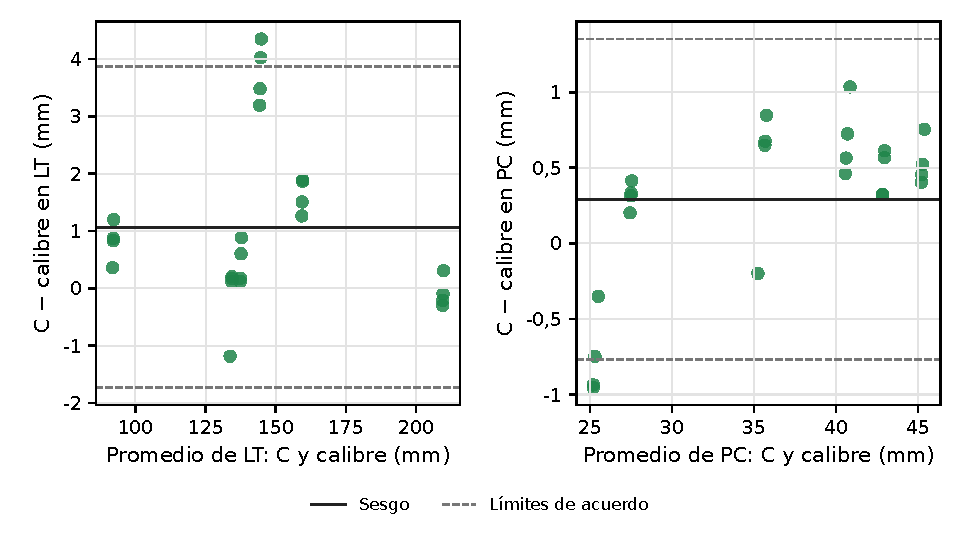
\includegraphics[width=0.95\textwidth]{fig4_bland_altman_c.pdf}
\caption[Bland--Altman de C frente al calibre]{Gráficos de Bland--Altman de C frente al calibre para LT (izquierda) y PC (derecha) sobre las 24 combinaciones réplica--profundidad. La línea continua indica el sesgo y las discontinuas los límites de acuerdo del 95~\%. Fuente: elaboración propia.}
\label{fig:4-BA}
\end{figure}

La Figura~\ref{fig:4-captura} muestra una de las capturas procesadas, con los cuatro puntos marcados y las estimaciones de cada ruta.

\begin{figure}[htbp]
\centering
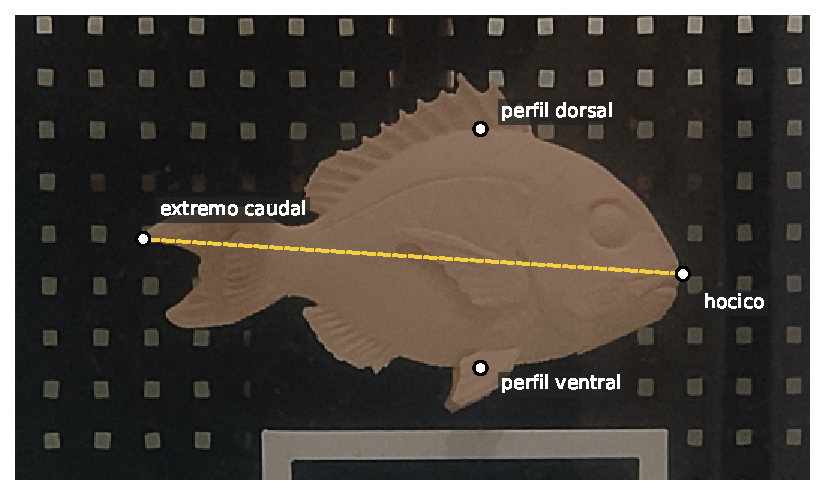
\includegraphics[width=0.9\textwidth]{fig4_captura_R3_230.pdf}
\caption[Captura real con los cuatro puntos anatómicos marcados]{Captura \texttt{R3-REP1-230.jpg} (réplica R3 a 23~cm del vidrio) con los cuatro puntos anatómicos marcados y el eje longitudinal. Referencia de calibre: LT 91,7~mm y PC 40,3~mm. Estimaciones de LT y PC: A, 55,4 y 24,5~mm; \Aprime, 93,7 y 41,6~mm; B, 91,7 y 40,1~mm; C, 92,6 y 40,7~mm. Fuente: elaboración propia.}
\label{fig:4-captura}
\end{figure}

\section{Alcance de los resultados}

Los resultados son válidos para las seis réplicas rígidas, la cámara Realme C71, la pecera de vidrio, las cuatro posiciones y las condiciones de iluminación utilizadas. No se generalizan directamente a peces vivos, movimiento, turbidez, oclusiones ni posiciones laterales que no fueron incluidas en la captura. Del mismo modo, las tres capturas técnicas no deben interpretarse como tres unidades experimentales independientes, y las 24 combinaciones réplica--profundidad no son 24 unidades: la unidad experimental es la réplica ($n = 6$).

En conjunto, los datos respaldan una ventaja de B y C, con la profundidad conocida, y en segundo lugar de \Aprime, frente a A para las medidas analizadas; entre B y C no se encontró diferencia en LT. Estas conclusiones se apoyan en la réplica como unidad y en referencias físicas de calibre. La conclusión se limita al flujo de procesamiento, al montaje y a las referencias físicas registradas.

\chapter{Conclusiones y recomendaciones}
\label{cap:conclusiones}

Empezamos con una pregunta práctica: ¿cómo medir un pez a través del vidrio de una pecera con una sola cámara? Para responderla pusimos a prueba, en un montaje controlado aire--vidrio--agua, cuatro rutas de conversión métrica sobre las mismas imágenes y los mismos puntos anatómicos, y medimos cuánto se ensancha la incertidumbre cuando no conocemos la profundidad. Trabajamos con seis réplicas rígidas de PLA, cuatro profundidades y tres capturas técnicas por condición: 72 imágenes en total. Todo lo que sigue se refiere a ese conjunto y a las referencias físicas registradas en el CSV maestro.

El aporte se puede condensar en una regla de decisión (Tabla~\ref{tab:regla} y Figura~\ref{fig:5-1}): según lo que se sepa de la escena, qué conversión conviene usar y cuánto error esperar en este montaje.

\begin{table}[htbp]
\centering\small
\caption{Regla de decisión: qué conversión usar según la situación, con el error observado en este montaje.}
\label{tab:regla}
\begin{tabularx}{\textwidth}{@{}X p{2.6cm} p{3.0cm} X@{}}
\toprule
Situación de uso & Método recomendado & Error esperado en este montaje & Condición \\
\midrule
Se puede poner un marcador junto al pez, en su mismo plano & \Aprime{} (homografía con marcador coplanar) & $\approx$ 2--3~\% de LT (3,3~mm) & Coplanaridad dentro de $\pm 1$~cm; no requiere calibración \\
No se puede poner un marcador junto al pez, pero se conoce su distancia al vidrio (riel, guía, tanque angosto) & C (puerto plano) & $< 1$~\% de LT (1,2~mm) & Calibración en aire y parámetros $d$, $t_g$ e índices del puerto \\
Hay calibración bajo agua en el mismo tanque y se conoce la posición del pez en el marco de esa calibración (riel o guía) & B (pinhole efectivo) & $< 1$~\% de LT (1,1~mm) & Damero sumergido y referencia del plano; comprobado hasta 18~cm de la zona calibrada \\
Marcador fijo en el vidrio y pez a distancia desconocida & Ninguno es aceptable (A) & 10--40~\% según la distancia & Solo sirve si el pez está pegado al vidrio \\
No se sabe nada de la profundidad & C con intervalo $\IL$ & 56--82~\% de ancho: no utilizable & Hay que acotar $z$; con $\pm 1$~cm el ancho baja a 4--5~\% \\
\bottomrule
\end{tabularx}
\end{table}

\begin{figure}[htbp]
\centering
\begin{tikzpicture}[>=Stealth,font=\small,
  preg/.style={draw,rounded corners=3pt,fill=gray!8,text width=5.2cm,align=center,minimum height=9mm},
  hoja/.style={draw,rounded corners=3pt,text width=4.6cm,align=center,minimum height=9mm,font=\small\bfseries}]
  \node[preg] (q1) at (0,0) {¿Se puede colocar un marcador coplanar con el pez?};
  \node[hoja,fill=metAp!15] (h1) at (6.3,0) {\Aprime\\ \normalfont error $\approx$ 2--3~\%};
  \node[preg] (q2) at (0,-2.2) {¿Se conoce la distancia pez--vidrio con $\pm 1$~cm?};
  \node[hoja,fill=metC!15] (h2) at (6.3,-2.2) {C, o B con calibración bajo agua\\ \normalfont error $< 1$~\%};
  \node[preg] (q3) at (0,-4.4) {¿Se puede acotar $z$ con una guía o una segunda vista?};
  \node[hoja,fill=metC!15] (h3) at (6.3,-4.4) {C con intervalo $\IL$\\ \normalfont ancho 4--17~\% según la cota};
  \node[hoja,fill=metA!15] (h4) at (0,-6.6) {No medir\\ \normalfont intervalo de 56--82~\%: no utilizable};
  \draw[->] (q1) -- node[above,font=\footnotesize]{sí} (h1);
  \draw[->] (q1) -- node[right,font=\footnotesize]{no} (q2);
  \draw[->] (q2) -- node[above,font=\footnotesize]{sí} (h2);
  \draw[->] (q2) -- node[right,font=\footnotesize]{no} (q3);
  \draw[->] (q3) -- node[above,font=\footnotesize]{sí} (h3);
  \draw[->] (q3) -- node[right,font=\footnotesize]{no} (h4);
\end{tikzpicture}
\caption[Diagrama de decisión para la conversión métrica monocular a través de un vidrio plano]{Diagrama de decisión para la conversión métrica monocular a través de un vidrio plano. Cada hoja indica el error observado en este montaje (Capítulo~\ref{cap:resultados}); B requiere una calibración bajo agua en el mismo tanque. Fuente: elaboración propia.}
\label{fig:5-1}
\end{figure}

\section{Conclusiones por objetivo}
\label{sec:conclusiones}

\begin{enumerate}
  \item \textbf{Conjunto de datos (objetivo 1).} Construimos y documentamos un conjunto de 72 imágenes de seis réplicas a cuatro profundidades, con referencias físicas de calibre, una tabla maestra que permite rastrear cada valor por réplica, profundidad, repetición e imagen, y un registro de exclusiones. Obtuvimos valores numéricos para 284 de los 288 registros; los cuatro restantes corresponden a A y \Aprime{} en dos imágenes en las que no se detectó el marcador. Resumimos las repeticiones técnicas por combinación réplica--profundidad. Objetivo cumplido.
  \item \textbf{Protocolo y repetibilidad del marcado (objetivo 2).} Definimos y aplicamos un protocolo de marcado manual único por imagen, con cuatro puntos anatómicos que comparten las cuatro rutas. No cuantificamos en esta versión la repetibilidad del marcado, que queda como verificación inmediata. Objetivo cumplido parcialmente.
  \item \textbf{Implementación y validación de las rutas (objetivo 3).} Implementamos las cuatro rutas en una aplicación propia de código abierto, con pruebas unitarias de sanidad para el módulo de puerto plano, y las evaluamos contra las referencias de calibre de las seis réplicas en 72 imágenes. B logró un MAE de 1,08~mm (0,73~\%) en LT y de 0,38~mm (1,26~\%) en PC; C, de 1,22~mm (0,88~\%) y 0,56~mm (1,62~\%); y \Aprime, de 3,29~mm (2,28~\%) y 1,03~mm (2,78~\%). No hicimos la comprobación instrumental con barra patrón. Objetivo cumplido en cuanto a la validación contra referencias físicas; la comprobación con patrón queda como trabajo futuro.
  \item \textbf{Comparación pareada según la separación (objetivo 4).} A fue la ruta más sensible a la profundidad: su MAE de LT pasó de 13,77~mm a 5~cm a 57,64~mm a 23~cm (2,43~mm por centímetro), tal como predice la geometría del puerto plano. B y C se mantuvieron entre 1,0 y 1,4~mm en las cuatro posiciones, sin tendencia con la separación. C superó a A y \Aprime{} en 6 de 6 réplicas ($p = 0{,}031$) y en 24 de 24 combinaciones, pero no se diferenció de B (3 de 6 réplicas, $p = 1$). H1 se sostiene frente a A y \Aprime{} y no frente a B. H2 no se sostiene: hasta 18~cm de la zona de calibración, B no se degradó con la separación. Objetivo cumplido.
  \item \textbf{Intervalo por profundidad desconocida (objetivo 5).} Calculamos el intervalo $\IL$ con C sobre las 72 capturas, y coincidió con la predicción geométrica del montaje (razón media 1,006). Su ancho es de 56--82~\% de LT si $z$ es desconocida en toda la pecera, de 11--16~\% con $\pm 3$~cm y de 4--5~\% con $\pm 1$~cm. La cobertura empírica fue de 1,00 en toda la pecera y con $\pm 3$~cm, y de 0,81 con $\pm 1$~cm. H3 se sostiene. Objetivo cumplido.
  \item \textbf{Sensibilidad (objetivo 6).} Cuantificamos cuánto depende C de la distancia cámara--vidrio y del índice del agua (Tabla~\ref{tab:sensibilidad}). Un error de $\pm 20$~\% en $d$ cambió la LT en 14~\% (cerca de 0,3~\% por milímetro); un cambio de $\pm 0{,}01$ en $\mu_w$, apenas 0,23~\%. No cuantificamos en esta versión la sensibilidad a la repetibilidad del marcado. Objetivo cumplido parcialmente.
\end{enumerate}

La Tabla~\ref{tab:cumplimiento} resume el grado de cumplimiento de cada objetivo.

\begin{table}[htbp]
\centering\small
\caption{Matriz de cumplimiento de los objetivos específicos.}
\label{tab:cumplimiento}
\begin{tabularx}{\textwidth}{@{}p{1.6cm} X p{1.8cm} X@{}}
\toprule
Objetivo & Resultado que lo sostiene & Grado & Pendiente \\
\midrule
1 & Tablas~\ref{tab:replicas} y~\ref{tab:registros}; repositorio & Cumplido & Publicar los datos con la etiqueta \texttt{\RepoTag} \\
2 & Sección~\ref{sec:procedimiento} & Parcial & Remarcado de doce imágenes \\
3 & Tablas~\ref{tab:calibraciones} y~\ref{tab:agregados} & Cumplido & Comprobación con barra patrón \\
4 & Tabla~\ref{tab:posiciones-mae}; Tabla~\ref{tab:hipotesis} & Cumplido & --- \\
5 & Tabla~\ref{tab:intervalo}; Figuras~\ref{fig:4-3} y~\ref{fig:4-Lz} & Cumplido & --- \\
6 & Tabla~\ref{tab:sensibilidad} & Parcial & Efecto del remarcado sobre las medidas \\
\bottomrule
\end{tabularx}
\end{table}

En pocas palabras: a través de un vidrio plano, la escala de un marcador pegado al vidrio no sirve para medir un pez que nada a otra profundidad, porque el error crece 2,4~mm por cada centímetro de separación. Un marcador en el plano del pez baja ese error a 2--3~\%. Un modelo de cámara calibrado, con la profundidad conocida, lo baja a menos del 1~\%, y da lo mismo si es el pinhole efectivo calibrado bajo el agua (B) o el puerto plano (C). Cuando la profundidad no se conoce, la geometría encierra la longitud en un intervalo demasiado ancho para hacer morfometría, salvo que la profundidad se acote a $\pm 1$~cm. En un sistema de una sola cámara, entonces, el problema a resolver es la profundidad, no la refracción, y este trabajo pone un número a cuánto pesa.

\section{Limitaciones}

Trabajamos con réplicas rígidas, una sola cámara y una pecera de vidrio, con la iluminación y el encuadre bajo control. No evaluamos peces vivos, movimiento, agua turbia, oclusiones ni posiciones laterales planificadas. Seis réplicas en una muestra no probabilística no alcanzan para generalizar a otras especies, tamaños, cámaras o puertos; las conclusiones valen para este montaje.

Hicimos la inferencia con una prueba de signos exacta sobre diferencias pareadas por réplica. No usamos pruebas paramétricas porque con $n = 6$ réplicas no se pueden verificar sus supuestos, y los conteos sobre 24 combinaciones son descriptivos. No hicimos la comprobación instrumental con barra patrón sumergida; la validación métrica es la comparación con las referencias de calibre. Tampoco cuantificamos en esta versión la repetibilidad del marcado, y por eso declaramos los objetivos 2 y 6 como parcialmente cumplidos.

\section{Recomendaciones}

Quien quiera repetir el procedimiento debería mantener fijos la cámara, la resolución, el enfoque, la iluminación, la posición de la pecera y la configuración del puerto durante todas las capturas, y conservar la imagen original, los puntos manuales, los archivos de calibración, la versión del programa y el registro de exclusiones. Recomendamos además registrar en cada sesión una medida física sumergida independiente, como una barra patrón, y repetir la evaluación con el pez en posiciones laterales del encuadre.

Para el uso práctico, la Tabla~\ref{tab:regla} resume qué hacer. La escala A es solo una línea de base y no corrige la refracción. B funciona si la posición del pez se expresa en el marco de su calibración y dentro del rango de distancias comprobado. C necesita conservar documentados los parámetros físicos del puerto, los índices de refracción y el sistema de coordenadas, y su salida solo es útil si la profundidad se conoce o se acota.

\section{Trabajos futuros}

\paragraph{Verificaciones inmediatas sobre este mismo conjunto.} Volver a marcar doce imágenes para medir la repetibilidad del operador, y hacer la comprobación con una barra patrón sumergida.

\paragraph{Líneas de continuación.} Quedan varios caminos abiertos. Detectar los puntos anatómicos de forma automática, con el mismo protocolo pareado, permitiría separar el error de localización del geométrico. Estimar la profundidad con una guía, una segunda vista o una restricción de postura reduciría el intervalo $\IL$ a un rango útil. También falta evaluar el método con peces vivos, agua turbia y posiciones fuera del centro del encuadre; incorporar al intervalo la incertidumbre de los parámetros del puerto y de los índices de refracción; y publicar un artículo con el conjunto de datos y el código.

\section{Impacto potencial y aporte}

El principal aporte de este trabajo es un procedimiento trazable para comparar conversiones métricas con una sola cámara en un montaje aire--vidrio--agua, y una medida concreta de lo que se puede afirmar sobre la longitud cuando no se conoce la profundidad. B y C fueron las rutas más exactas, con errores menores que el 1~\% cuando la profundidad es conocida, y \Aprime{} ofrece una alternativa más simple que mejora mucho a la escala fija en el vidrio.

Para la Ingeniería Informática, el trabajo deja cuatro productos: (1) un módulo de trazado refractivo de puerto plano, implementado a partir de las formulaciones de \textcite{Agrawal2012} y \textcite{Treibitz2012}, con pruebas unitarias de sanidad (con $\mu_g = \mu_w = 1$ y $t_g = 0$ reproduce la cámara pinhole) y evaluado contra referencias físicas; (2) una aplicación de escritorio de código abierto que conserva la trazabilidad de cada imagen (puntos, calibración, versión y advertencias) y exporta un registro reproducible; (3) un procedimiento experimental pareado que aísla el efecto del modelo geométrico y que sirve para evaluar, en el futuro, detectores automáticos de puntos; y (4) evidencia cuantitativa, para este montaje, sobre cuándo alcanza un marcador, cuándo conviene una calibración bajo el agua y cuándo hace falta el modelo físico.

Para la acuicultura, el resultado es una regla práctica, con números, para medir peces sin sacarlos del agua usando una cámara común a través del vidrio de un tanque. Llevarla a peces vivos o a instalaciones productivas sigue siendo una posibilidad futura, que requiere validarla primero en esas condiciones.


% ================= REFERENCIAS =================
\clearpage
\phantomsection
\addcontentsline{toc}{chapter}{Referencias}
\printbibliography[title={Referencias}]

% ================= ANEXOS =================
\appendix
% Figura A1, Tabla F1, Listado C1: número propio dentro de cada anexo (APA)
\counterwithin*{figure}{chapter}
\counterwithin*{table}{chapter}
\counterwithin*{lstlisting}{chapter}
\renewcommand{\thefigure}{\thechapter\arabic{figure}}
\renewcommand{\thetable}{\thechapter\arabic{table}}
\renewcommand{\thelstlisting}{\thechapter\arabic{lstlisting}}
\chapter*{Anexos}
\addcontentsline{toc}{chapter}{Anexos}

Los anexos reúnen el material de respaldo del experimento: el registro visual de las capturas, la configuración del puerto plano, los perfiles de calibración, la referencia geométrica del riel, la estructura de los repositorios de código y datos, la tabla maestra de resultados, las fichas de las réplicas y las fotografías del montaje y de los instrumentos. Los archivos completos están publicados con los datos del experimento (Anexo~\ref{anx:repositorio}); aquí se muestran sus campos principales para facilitar la lectura y la trazabilidad.

\chapter{Registro visual de capturas}
\label{anx:capturas}

La Figura~\ref{fig:A-1} reúne en una sola vista las capturas del experimento. Cada etiqueta indica la réplica, la repetición y la distancia nominal de la réplica al vidrio en milímetros; por ejemplo, \texttt{R1-REP1-50.jpg}. La vista permite comprobar la organización del conjunto y la correspondencia de cada captura con su posición. Las 72 imágenes originales están publicadas en el repositorio de datos (Anexo~\ref{anx:repositorio}).

\begin{figure}[H]
\centering
\caption[Vista conjunta de las capturas y sus identificadores]{Vista conjunta de las capturas y sus identificadores.}
\label{fig:A-1}
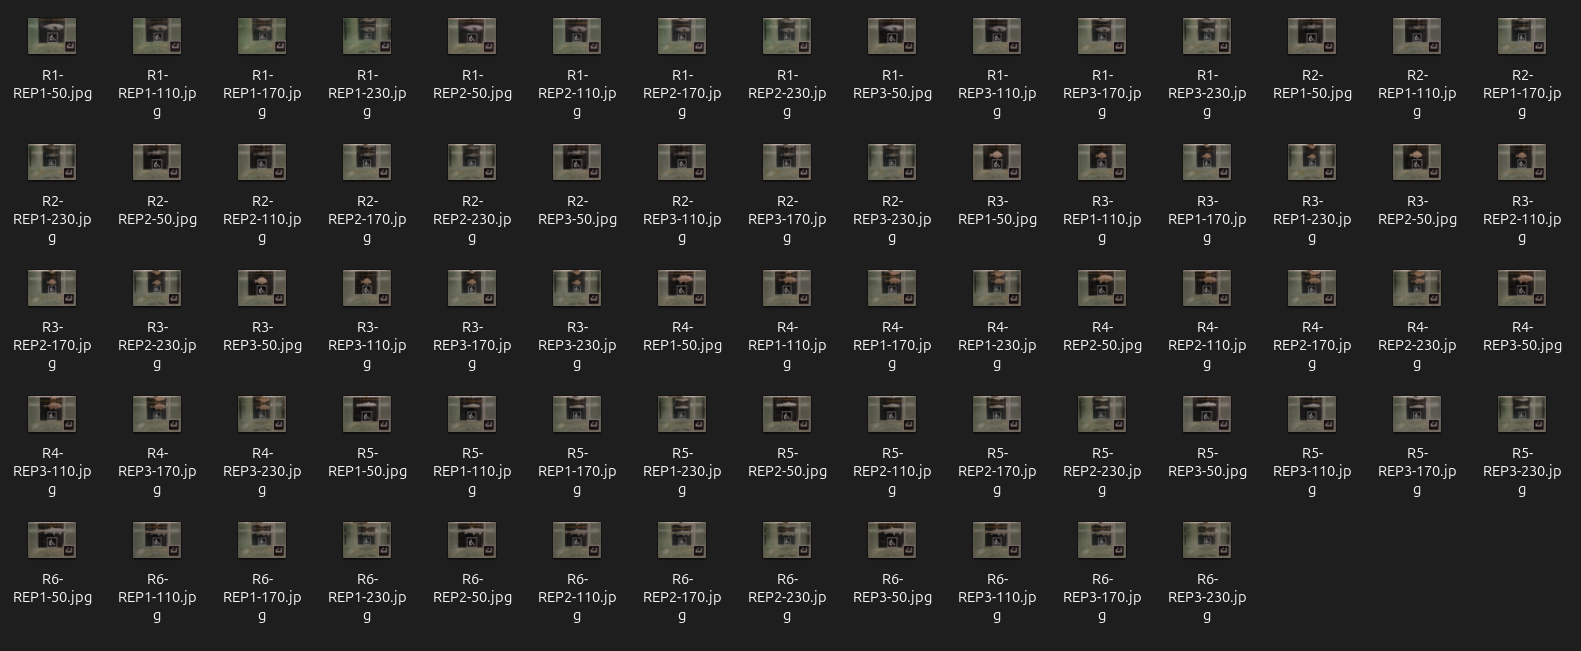
\includegraphics[width=\textwidth]{figA_1_capturas.png}
\fignota{Elaboración propia.}
\end{figure}

\chapter{Configuración del puerto plano}
\label{anx:flatport}

La Figura~\ref{fig:B-1} reproduce la configuración del modelo de puerto plano, resumida en la Tabla~\ref{tab:puerto}: unidades en milímetros, normal de cámara $(0, 0, 1)$, distancia de la interfaz de 230~mm, vidrio de 4~mm de espesor e índices de refracción de 1,000 para el aire, 1,500 para el vidrio y 1,333 para el agua. El archivo deja constancia de que la distancia de la lente se midió desde su frente, como aproximación, y de que el agua estaba a 22~\si{\celsius}, con salinidad 0 y presión 0~dbar.

\begin{figure}[H]
\centering
\caption[Parámetros visibles de la configuración del puerto plano]{Parámetros visibles de la configuración del puerto plano.}
\label{fig:B-1}
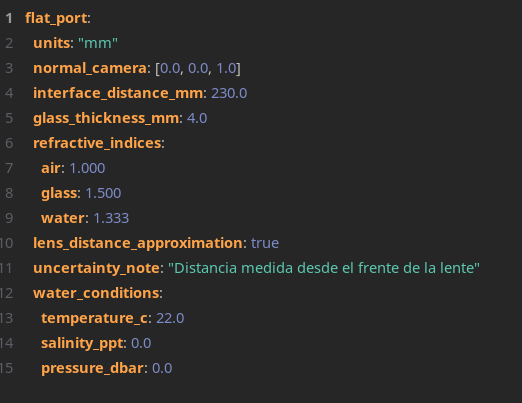
\includegraphics[width=0.6\textwidth]{figB_1_flatport.png}
\fignota{Captura de pantalla de Fishmeter, aplicación desarrollada en este trabajo.}
\end{figure}

\chapter{Parámetros de calibración de cámara}
\label{anx:calibraciones}

Los archivos \texttt{calibration\_B.yaml} y \texttt{calibration\_C\_air.yaml} guardan los perfiles de calibración de las rutas B y C. Los dos usan el modelo de cámara de OpenCV, una resolución de $4096 \times 3072$ píxeles y un tablero de $4 \times 4$ esquinas interiores con cuadros de 20~mm. La Tabla~\ref{tab:calibraciones} presenta sus indicadores de calidad. Los listados que siguen reproducen la cabecera y el resumen de cada archivo; los informes de cada vista quedan en los YAML completos, publicados con los datos (Anexo~\ref{anx:repositorio}).

\begin{lstlisting}[caption={Cabecera y resumen del perfil B.},label={lst:calB}]
schema: fish_morphometry.b_calibration.v1
profile_id: B-effective
profile_hash: eb245104cb46caded48e9e9f827dda11db985c7b22ec5cb63a27572da14caf4e
calibration_context_hash: 1e3531dcf0d9ff8d00b322b41d2dd074b41cb822a1324cd5545635303ca81ba6
model: OPENCV
camera_matrix:
- [4502.32284117, 0.0, 2027.2736574393155]
- [0.0, 4504.395746404586, 1549.0026630316365]
- [0.0, 0.0, 1.0]
distortion_coefficients:
- 0.4454686711747631
- -3.4668133596510753
- -0.008336348094703296
- 0.004790603340447537
- 8.25240238252019
resolution: [4096, 3072]
calibration_rail_position_mm: 0.0
created_at_utc: '2026-10-12T04:07:10.722788+00:00'
versions:
  opencv: 5.0.0
  fish_morphometry: 0.1.0
source: opencv_calibrateCamera
board:
  inner_corners: [4, 4]
  square_size_mm: 20.0
rms_px: 0.4353568098178903
views:
  received: 35
  accepted: 35
  rejected: 0
\end{lstlisting}

\begin{lstlisting}[caption={Cabecera y resumen del perfil C en aire.},label={lst:calC}]
schema: fish_morphometry.air_calibration.v1
profile_id: C-air
profile_hash: fb98aea6af6ba57d663f5884b4034bfff3413c62cc376bef82256a7c1f412a55
calibration_context_hash: 623631f83c66f4b1615fd73e2f4db719880ccaa11c117bc705674d1a0df96ef8
model: OPENCV
camera_matrix:
- [3313.72125140631, 0.0, 2028.1975106019397]
- [0.0, 3313.6744263215105, 1530.5739559303083]
- [0.0, 0.0, 1.0]
distortion_coefficients:
- 0.18564347583186028
- -0.829350911254369
- -0.0011635185172718578
- -0.0015902497923188043
- 1.0012733784385703
resolution: [4096, 3072]
board:
  inner_corners: [4, 4]
  square_size_mm: 20.0
  units: mm
rms_px: 0.3745461951579489
created_at_utc: '2026-10-12T04:12:38.034127+00:00'
versions:
  opencv: 5.0.0
  fish_morphometry: 0.1.0
source: opencv_calibrateCamera_air
views:
  received: 36
  accepted: 36
  rejected: 0
\end{lstlisting}

\chapter{Referencia geométrica del riel para B}
\label{anx:riel}

El archivo \texttt{rail\_reference\_B.yaml} documenta el plano de referencia de B, obtenido a partir de dos posiciones del riel, 0 y 180~mm, con un error de reproyección de 0,270~px (umbral de 1,0~px). El ajuste informa un residuo lineal de $1{,}62 \times 10^{-13}$~mm, que es el residuo numérico de una recta por dos puntos y no representa la incertidumbre física; una dispersión de la normal de $0{,}337^{\circ}$ (umbral de $1{,}0^{\circ}$); y un error relativo de escala de 0,813~\% (umbral de 5~\%). El archivo registra además dos supuestos: los planos de las réplicas son paralelos al tablero, y el riel no es necesariamente perpendicular a él. La Tabla~\ref{tab:riel} resume los valores principales.

\begin{lstlisting}[caption={Cabecera y plano de referencia del riel para B.},label={lst:riel}]
plane_point_camera_mm:
- -34.117491789288806
- -28.291160700295567
- 365.1469994117171
plane_normal_camera:
- -0.03972877728543376
- -0.042783728187314775
- 0.9982941334385363
z_ref_mm: 0.0
rail_direction_camera:
- 0.02095849070805215
- -0.04478647483729878
- 0.998776708448334
\end{lstlisting}

\chapter{Repositorio de código y datos}
\label{anx:repositorio}

El trabajo está publicado en dos repositorios. El código de Fishmeter está en \url{\RepoURL}, etiqueta \texttt{\RepoTag}, que corresponde al commit\par\noindent{\footnotesize\texttt{\RepoCommit}}\par
\noindent Los datos del experimento y los scripts que regeneran las tablas y figuras del Capítulo~\ref{cap:resultados} están en el repositorio de este documento, \url{\DatosURL}, etiqueta \texttt{\DatosTag}, que corresponde al commit\par\noindent{\footnotesize\texttt{\DatosCommit}}\par\noindent La estructura de ambos es la siguiente:

\begin{lstlisting}
FishmeterTPF/                     codigo (etiqueta v1.0-tesis)
  src/fish_morphometry/           aplicacion Fishmeter (calibracion, geometria,
                                  metodos A, A', B y C, interfaz, validacion)
  tests/                          pruebas unitarias e integracion (pytest)
  docs/                           guia de uso y notas de desarrollo
  README.md                       instalacion y ejecucion

ProyectoTPF/                      datos y analisis
  datos/imagenes/                 72 imagenes JPG originales
  datos/calibraciones/            perfiles B y C, puerto plano y riel (YAML)
  datos/referencias/replicas.csv  tres lecturas de calibre por medida
  datos/resultados_json/          un JSON por imagen y metodo (puntos y parametros)
  datos/derivados/                L(z), intervalos y sensibilidad de C
  datos/SHA256SUMS                huellas de todos los archivos de datos
  datos/README.md                 contenido y convenciones de los datos
  anexos/csv-maestro-re-run.csv   tabla maestra (288 registros)
  analysis/reproducir_capitulo4.py  Tablas 4.3 a 4.6, pruebas de signos,
                                  Bland-Altman y Figuras 4.5 y 4.6
  analysis/make_figures.py        Figuras 4.1 a 4.4 y 4.7
  analysis/tabla_maestra.py       tabla del Anexo F
  analysis/re_run_b.py            recalculo de B con la lectura del riel
\end{lstlisting}

Para reproducir el Capítulo~\ref{cap:resultados} se debe instalar Fishmeter en la versión indicada y ejecutar, desde la raíz de ProyectoTPF, los tres primeros scripts de \texttt{analysis/} en el orden del listado. El primero recalcula C desde los puntos marcados con el perfil \texttt{C-air} y la configuración del puerto plano; los otros dos leen la tabla maestra, los resultados del primero y, para la Figura~\ref{fig:4-captura}, la imagen original. El cuarto, \texttt{re\_run\_b.py}, documenta cómo se obtuvieron los valores de B de la tabla maestra: toma los JSON de B del cálculo preliminar y repite el cálculo con la posición expresada en el marco del riel (Anexo~\ref{anx:riel}), sin cambiar los puntos marcados ni las calibraciones. Su salida ya está incluida en la tabla maestra, por lo que no es necesario ejecutarlo para reproducir el capítulo.

\chapter{Tabla maestra de resultados}
\label{anx:maestra}

La Tabla~\ref{tab:maestra} reproduce, para cada una de las 72 imágenes, las referencias de calibre y las estimaciones de LT y PC de los cuatro métodos; el error con signo de cada estimación es su diferencia con la referencia. Los guiones marcan los cuatro registros sin valor, en los que no se detectó el ArUco (Sección~\ref{sec:conjunto}). La tabla se generó con \texttt{analysis/tabla\_maestra.py} a partir del CSV maestro, que guarda además los puntos marcados (con $\mathbf{p}_1$ y $\mathbf{p}_2$ invertidos respecto de la definición de la Sección~\ref{sec:medidas}), los parámetros de cada ruta y sus advertencias. Su huella SHA-256 figura a continuación de la tabla.

% Generado por analysis/tabla_maestra.py; no editar a mano.
% CSV: csv-maestro-re-run.csv, SHA-256 f5e8c1091ceb06ec406dffc0d1a02f5b65f9147fdf5a582671e33e65abf8235c
\newcommand{\MaestraSHA}{f5e8c1091ceb06ec406dffc0d1a02f5b65f9147fdf5a582671e33e65abf8235c}
\begin{footnotesize}
\setlength{\tabcolsep}{4pt}
\begin{longtable}{@{}lrrrrrrrrrr@{}}
\caption{Tabla maestra: referencias de calibre y estimaciones por imagen y método.}
\label{tab:maestra}\\
\toprule
 & \multicolumn{5}{c}{Longitud total (mm)} & \multicolumn{5}{c}{Profundidad corporal (mm)} \\
\cmidrule(lr){2-6}\cmidrule(l){7-11}
Imagen & Ref. & A & \Aprime & B & C & Ref. & A & \Aprime & B & C \\
\midrule
\endfirsthead
\toprule
 & \multicolumn{5}{c}{Longitud total (mm)} & \multicolumn{5}{c}{Profundidad corporal (mm)} \\
\cmidrule(lr){2-6}\cmidrule(l){7-11}
Imagen & Ref. & A & \Aprime & B & C & Ref. & A & \Aprime & B & C \\
\midrule
\endhead
\bottomrule
\endfoot
\texttt{R1-REP1-50} & 158,7 & 143,0 & 161,8 & 162,7 & 164,1 & 45,0 & 41,0 & 45,6 & 45,9 & 46,8 \\
\texttt{R1-REP2-50} & 158,7 & 143,2 & 164,7 & 156,9 & 158,1 & 45,0 & 40,8 & 46,7 & 44,2 & 45,0 \\
\texttt{R1-REP3-50} & 158,7 & 142,7 & 163,8 & 156,4 & 157,6 & 45,0 & 41,3 & 47,5 & 44,7 & 45,5 \\
\texttt{R1-REP1-110} & 158,7 & 123,0 & 163,3 & 163,6 & 164,7 & 45,0 & 34,7 & 45,7 & 45,6 & 46,3 \\
\texttt{R1-REP2-110} & 158,7 & 123,2 & 162,4 & 157,3 & 158,4 & 45,0 & 35,2 & 46,1 & 44,5 & 45,2 \\
\texttt{R1-REP3-110} & 158,7 & 123,4 & 161,8 & 157,5 & 158,6 & 45,0 & 35,0 & 45,3 & 44,3 & 45,0 \\
\texttt{R1-REP1-170} & 158,7 & 106,9 & 164,1 & 162,2 & 163,3 & 45,0 & 30,2 & 45,9 & 45,2 & 45,9 \\
\texttt{R1-REP2-170} & 158,7 & 108,1 & 162,6 & 157,7 & 158,8 & 45,0 & 30,8 & 46,4 & 44,6 & 45,3 \\
\texttt{R1-REP3-170} & 158,7 & 108,5 & 163,5 & 158,4 & 159,5 & 45,0 & 30,7 & 46,1 & 44,4 & 45,1 \\
\texttt{R1-REP1-230} & 158,7 & 94,5 & 163,5 & 161,3 & 162,5 & 45,0 & 26,5 & 45,6 & 44,8 & 45,5 \\
\texttt{R1-REP2-230} & 158,7 & 95,9 & 161,9 & 157,6 & 158,9 & 45,0 & 27,4 & 46,1 & 44,8 & 45,5 \\
\texttt{R1-REP3-230} & 158,7 & 96,0 & 162,5 & 157,9 & 159,1 & 45,0 & 27,3 & 45,9 & 44,5 & 45,2 \\
\texttt{R2-REP1-50} & 134,3 & 119,1 & 136,5 & 131,2 & 132,1 & 27,3 & 24,6 & 28,2 & 26,5 & 27,0 \\
\texttt{R2-REP2-50} & 134,3 & 120,4 & 135,0 & 132,6 & 133,5 & 27,3 & 25,5 & 28,4 & 27,5 & 28,0 \\
\texttt{R2-REP3-50} & 134,3 & 120,6 & 136,5 & 132,9 & 133,8 & 27,3 & 25,1 & 28,4 & 27,0 & 27,5 \\
\texttt{R2-REP1-110} & 134,3 & 103,6 & 135,1 & 133,2 & 134,1 & 27,3 & 21,6 & 28,0 & 27,2 & 27,6 \\
\texttt{R2-REP2-110} & 134,3 & 104,6 & 136,7 & 134,3 & 135,2 & 27,3 & 21,5 & 28,1 & 27,0 & 27,5 \\
\texttt{R2-REP3-110} & 134,3 & 103,7 & 135,1 & 133,3 & 134,2 & 27,3 & 21,7 & 28,1 & 27,4 & 27,8 \\
\texttt{R2-REP1-170} & 134,3 & 90,6 & 137,0 & 133,1 & 134,1 & 27,3 & 18,7 & 28,3 & 26,9 & 27,4 \\
\texttt{R2-REP2-170} & 134,3 & --- & --- & 133,5 & 134,5 & 27,3 & --- & --- & 27,1 & 27,6 \\
\texttt{R2-REP3-170} & 134,3 & 91,0 & 135,5 & 133,8 & 134,8 & 27,3 & 19,1 & 28,3 & 27,6 & 28,0 \\
\texttt{R2-REP1-230} & 134,3 & 80,7 & 135,8 & 133,4 & 134,5 & 27,3 & 16,9 & 28,4 & 27,5 & 27,9 \\
\texttt{R2-REP2-230} & 134,3 & 80,6 & 136,0 & 133,2 & 134,3 & 27,3 & 16,6 & 28,2 & 26,9 & 27,4 \\
\texttt{R2-REP3-230} & 134,3 & 80,9 & 135,0 & 133,6 & 134,8 & 27,3 & 16,9 & 28,1 & 27,5 & 27,9 \\
\texttt{R3-REP1-50} & 91,7 & 82,6 & 93,8 & 91,2 & 91,8 & 40,3 & 37,0 & 42,5 & 40,2 & 40,9 \\
\texttt{R3-REP2-50} & 91,7 & --- & --- & 91,4 & 92,0 & 40,3 & --- & --- & 40,1 & 40,8 \\
\texttt{R3-REP3-50} & 91,7 & 83,0 & 93,8 & 91,6 & 92,2 & 40,3 & 36,9 & 41,9 & 40,1 & 40,7 \\
\texttt{R3-REP1-110} & 91,7 & 71,4 & 94,2 & 91,9 & 92,6 & 40,3 & 31,5 & 41,5 & 40,0 & 40,6 \\
\texttt{R3-REP2-110} & 91,7 & 71,4 & 93,2 & 91,9 & 92,6 & 40,3 & 32,1 & 41,4 & 40,7 & 41,4 \\
\texttt{R3-REP3-110} & 91,7 & 71,2 & 93,2 & 91,8 & 92,5 & 40,3 & 31,9 & 41,6 & 40,5 & 41,2 \\
\texttt{R3-REP1-170} & 91,7 & 62,1 & 93,1 & 91,5 & 92,3 & 40,3 & 28,0 & 41,8 & 40,7 & 41,3 \\
\texttt{R3-REP2-170} & 91,7 & 62,4 & 93,9 & 91,9 & 92,6 & 40,3 & 28,0 & 42,2 & 40,7 & 41,3 \\
\texttt{R3-REP3-170} & 91,7 & 62,3 & 93,6 & 91,8 & 92,6 & 40,3 & 28,1 & 42,0 & 40,8 & 41,5 \\
\texttt{R3-REP1-230} & 91,7 & 55,4 & 93,7 & 91,7 & 92,6 & 40,3 & 24,5 & 41,6 & 40,1 & 40,7 \\
\texttt{R3-REP2-230} & 91,7 & 55,9 & 93,3 & 92,4 & 93,3 & 40,3 & 24,7 & 41,1 & 40,3 & 40,9 \\
\texttt{R3-REP3-230} & 91,7 & 55,4 & 93,3 & 91,8 & 92,7 & 40,3 & 24,7 & 41,3 & 40,4 & 41,1 \\
\texttt{R4-REP1-50} & 142,7 & 130,5 & 149,3 & 143,5 & 144,5 & 42,7 & 39,0 & 44,6 & 42,0 & 42,8 \\
\texttt{R4-REP2-50} & 142,7 & 132,5 & 150,1 & 145,9 & 146,9 & 42,7 & 39,7 & 45,2 & 42,7 & 43,6 \\
\texttt{R4-REP3-50} & 142,7 & 133,0 & 148,9 & 146,1 & 147,1 & 42,7 & 39,6 & 44,2 & 42,6 & 43,4 \\
\texttt{R4-REP1-110} & 142,7 & 113,7 & 148,7 & 145,9 & 146,8 & 42,7 & 33,5 & 43,6 & 42,2 & 42,9 \\
\texttt{R4-REP2-110} & 142,7 & 114,1 & 148,7 & 146,1 & 147,0 & 42,7 & 33,6 & 43,6 & 42,2 & 42,9 \\
\texttt{R4-REP3-110} & 142,7 & 114,0 & 148,8 & 146,3 & 147,2 & 42,7 & 34,2 & 44,3 & 43,1 & 43,9 \\
\texttt{R4-REP1-170} & 142,7 & 99,4 & 148,5 & 145,7 & 146,7 & 42,7 & 29,6 & 44,5 & 42,7 & 43,3 \\
\texttt{R4-REP2-170} & 142,7 & 99,3 & 149,0 & 145,7 & 146,7 & 42,7 & 29,3 & 43,9 & 42,2 & 42,9 \\
\texttt{R4-REP3-170} & 142,7 & 99,5 & 149,1 & 145,7 & 146,7 & 42,7 & 29,2 & 43,7 & 42,0 & 42,7 \\
\texttt{R4-REP1-230} & 142,7 & 87,4 & 147,6 & 144,3 & 145,4 & 42,7 & 25,9 & 43,3 & 42,1 & 42,7 \\
\texttt{R4-REP2-230} & 142,7 & 88,4 & 148,3 & 145,8 & 146,9 & 42,7 & 26,4 & 44,0 & 42,8 & 43,5 \\
\texttt{R4-REP3-230} & 142,7 & 87,3 & 147,4 & 144,1 & 145,2 & 42,7 & 25,9 & 43,6 & 42,1 & 42,8 \\
\texttt{R5-REP1-50} & 137,3 & 123,8 & 139,1 & 136,3 & 137,2 & 25,7 & 22,4 & 25,0 & 24,1 & 24,6 \\
\texttt{R5-REP2-50} & 137,3 & 124,2 & 139,6 & 136,5 & 137,4 & 25,7 & 22,8 & 25,6 & 24,5 & 25,0 \\
\texttt{R5-REP3-50} & 137,3 & 124,5 & 140,3 & 136,8 & 137,8 & 25,7 & 23,0 & 26,0 & 24,7 & 25,2 \\
\texttt{R5-REP1-110} & 137,3 & 106,8 & 139,7 & 137,1 & 138,1 & 25,7 & 19,8 & 26,2 & 24,9 & 25,4 \\
\texttt{R5-REP2-110} & 137,3 & 106,9 & 141,3 & 137,3 & 138,3 & 25,7 & 19,6 & 25,9 & 24,5 & 25,0 \\
\texttt{R5-REP3-110} & 137,3 & 107,2 & 140,5 & 137,3 & 138,3 & 25,7 & 20,0 & 26,1 & 25,1 & 25,6 \\
\texttt{R5-REP1-170} & 137,3 & 93,3 & 139,6 & 136,9 & 137,9 & 25,7 & 16,9 & 25,3 & 24,3 & 24,8 \\
\texttt{R5-REP2-170} & 137,3 & 93,3 & 139,9 & 136,7 & 137,7 & 25,7 & 17,1 & 25,6 & 24,6 & 25,0 \\
\texttt{R5-REP3-170} & 137,3 & 93,6 & 140,7 & 137,1 & 138,1 & 25,7 & 16,7 & 25,0 & 24,0 & 24,4 \\
\texttt{R5-REP1-230} & 137,3 & 82,7 & 140,8 & 136,7 & 137,9 & 25,7 & 14,8 & 25,4 & 24,0 & 24,5 \\
\texttt{R5-REP2-230} & 137,3 & 82,0 & 138,9 & 135,4 & 136,6 & 25,7 & 15,1 & 25,3 & 24,4 & 24,8 \\
\texttt{R5-REP3-230} & 137,3 & 82,9 & 139,4 & 136,7 & 137,9 & 25,7 & 15,1 & 25,2 & 24,4 & 24,8 \\
\texttt{R6-REP1-50} & 209,7 & 189,8 & 213,2 & 208,7 & 210,0 & 35,3 & 33,6 & 37,8 & 36,2 & 36,9 \\
\texttt{R6-REP2-50} & 209,7 & 189,7 & 212,2 & 208,0 & 209,3 & 35,3 & 32,8 & 36,3 & 35,3 & 36,0 \\
\texttt{R6-REP3-50} & 209,7 & 189,6 & 212,6 & 208,1 & 209,4 & 35,3 & 32,5 & 36,2 & 35,0 & 35,7 \\
\texttt{R6-REP1-110} & 209,7 & 162,3 & 212,7 & 207,7 & 208,7 & 35,3 & 28,7 & 37,7 & 36,2 & 36,8 \\
\texttt{R6-REP2-110} & 209,7 & 163,0 & 212,3 & 208,5 & 209,6 & 35,3 & 27,6 & 35,9 & 34,7 & 35,3 \\
\texttt{R6-REP3-110} & 209,7 & 163,4 & 212,4 & 208,8 & 209,8 & 35,3 & 28,1 & 36,6 & 35,3 & 35,9 \\
\texttt{R6-REP1-170} & 209,7 & 142,8 & 211,2 & 208,8 & 209,9 & 35,3 & 25,3 & 36,9 & 36,5 & 37,1 \\
\texttt{R6-REP2-170} & 209,7 & 142,9 & 213,9 & 208,8 & 209,9 & 35,3 & 24,5 & 36,7 & 35,3 & 35,8 \\
\texttt{R6-REP3-170} & 209,7 & 143,2 & 213,4 & 209,0 & 210,1 & 35,3 & 23,9 & 35,1 & 34,4 & 35,0 \\
\texttt{R6-REP1-230} & 209,7 & 127,0 & 216,0 & 208,8 & 210,1 & 35,3 & 21,3 & 36,4 & 34,7 & 35,2 \\
\texttt{R6-REP2-230} & 209,7 & 126,4 & 214,2 & 208,3 & 209,6 & 35,3 & 21,1 & 35,3 & 34,4 & 35,0 \\
\texttt{R6-REP3-230} & 209,7 & 126,2 & 211,5 & 207,4 & 208,7 & 35,3 & 21,4 & 35,5 & 34,7 & 35,2 \\
\end{longtable}
\end{footnotesize}


\noindent{\footnotesize SHA-256 del CSV maestro:\\ \texttt{\MaestraSHA}}

\chapter{Fichas de las réplicas}
\label{anx:fichas}

Las seis réplicas están impresas en PLA. La Figura~\ref{fig:G-1} las muestra juntas, cada una con su identificador, y la Tabla~\ref{tab:lecturas-calibre} reproduce las tres lecturas de calibre de cada medida, registradas al milímetro, con su media y su desviación estándar muestral; las medias son las referencias de la Tabla~\ref{tab:replicas}.

\begin{figure}[H]
\centering
\caption[Réplicas utilizadas en el experimento con su identificador]{Las seis réplicas impresas en PLA, con el identificador (R1--R6) que se usa en todo el documento.}
\label{fig:G-1}
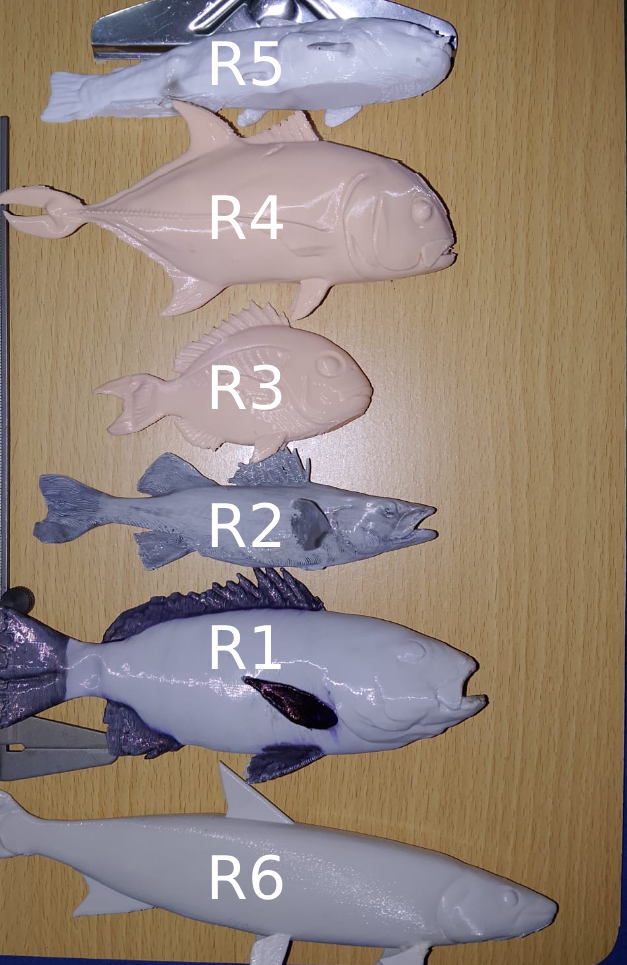
\includegraphics[width=0.55\textwidth]{fig3_1_replicas_tags.jpg}
\fignota{Elaboración propia.}
\end{figure}

\begin{table}[H]
\centering\footnotesize
\caption{Lecturas de calibre de las réplicas (mm).}
\label{tab:lecturas-calibre}
\begin{tabular}{@{}lccccc@{\hspace{1.2em}}ccccc@{}}
\toprule
 & \multicolumn{5}{c}{Longitud total (LT)} & \multicolumn{5}{c}{Profundidad corporal (PC)} \\
\cmidrule(lr){2-6}\cmidrule(l){7-11}
Réplica & 1 & 2 & 3 & Media & Desv. & 1 & 2 & 3 & Media & Desv. \\
\midrule
R1 & 160 & 157 & 159 & 158,7 & 1,5 & 45 & 45 & 45 & 45,0 & 0,0 \\
R2 & 131 & 136 & 136 & 134,3 & 2,9 & 28 & 27 & 27 & 27,3 & 0,6 \\
R3 & 91  & 92  & 92  & 91,7  & 0,6 & 41 & 40 & 40 & 40,3 & 0,6 \\
R4 & 141 & 146 & 141 & 142,7 & 2,9 & 43 & 42 & 43 & 42,7 & 0,6 \\
R5 & 137 & 138 & 137 & 137,3 & 0,6 & 25 & 26 & 26 & 25,7 & 0,6 \\
R6 & 210 & 209 & 210 & 209,7 & 0,6 & 35 & 36 & 35 & 35,3 & 0,6 \\
\bottomrule
\end{tabular}

\smallskip
\begin{minipage}{0.9\textwidth}\footnotesize
\emph{Nota.} Las lecturas de PC de R1 y R2 se anotaron originalmente con un cero de más (450 por 45~mm; 280/270/270 por 28/27/27~mm) y se corrigieron antes del análisis; la corrección está registrada en \texttt{datos/referencias/replicas.csv} y en la tabla maestra.
\end{minipage}
\end{table}

\chapter{Montaje e instrumentos}
\label{anx:montaje}

La Figura~\ref{fig:H-1} muestra la pecera de vidrio en la que se hizo el ensayo, con agua y el soporte de PLA en su interior; sus dimensiones y la disposición del montaje están en la Sección~\ref{sec:montaje} y en la Figura~\ref{fig:3-esquema}. La Figura~\ref{fig:H-2} reúne los instrumentos con los que se midió y se armó el montaje: las reglas y la escuadra con las que se midió la distancia cámara--vidrio y se comprobó la perpendicularidad de la cámara, el calibre analógico con el que se tomaron las medidas de referencia, el damero de calibración, los dos marcadores ArUco, el soporte del teléfono y los útiles con los que se cortaron y fijaron las piezas.

\begin{figure}[H]
\centering
\caption[Pecera utilizada en el experimento]{Pecera de vidrio utilizada en el experimento, con agua y el soporte de PLA en su interior.}
\label{fig:H-1}
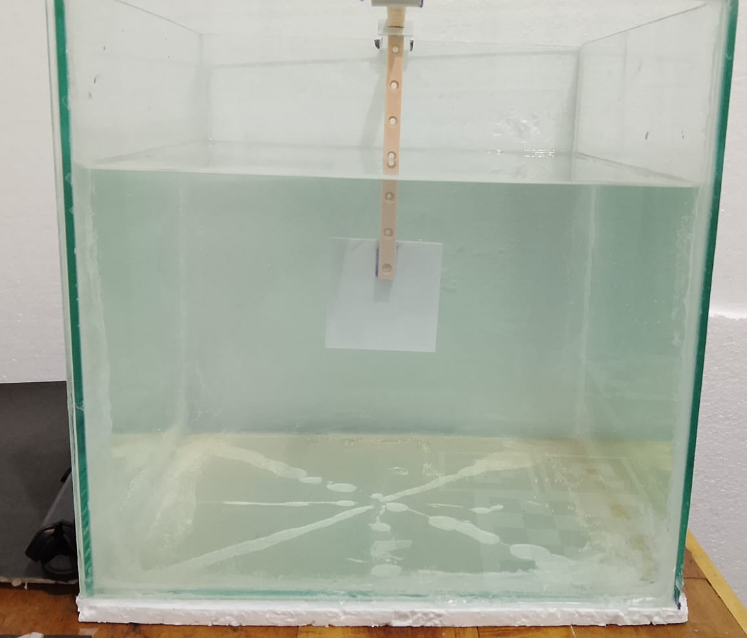
\includegraphics[width=0.48\textwidth]{estanque.png}
\fignota{Elaboración propia.}
\end{figure}

\begin{figure}[H]
\centering
\caption[Instrumentos de medición y de manipulación]{Instrumentos de medición y de manipulación: reglas, escuadra, calibre, damero de calibración, marcadores ArUco, soporte del teléfono, cinta doble faz y herramientas de corte y sujeción.}
\label{fig:H-2}
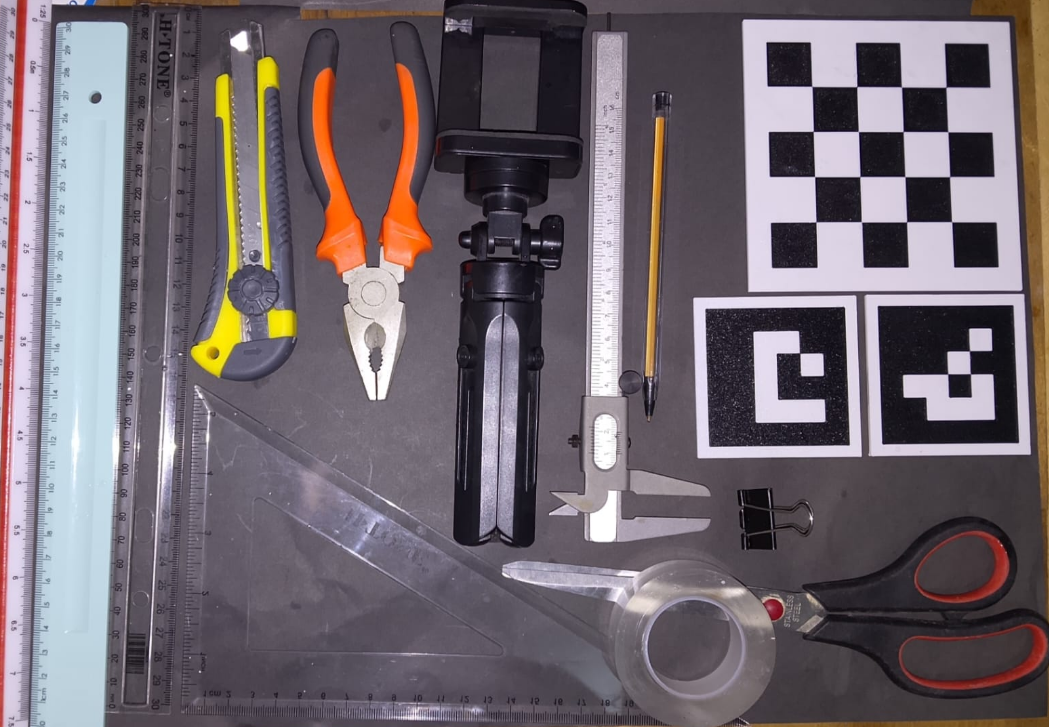
\includegraphics[width=0.65\textwidth]{tools-measure-manipulate.png}
\fignota{Elaboración propia.}
\end{figure}


% ---------------------------------------------------------------------------
% Registro de cambios: comentado para la entrega. Para mostrarlo de nuevo,
% seleccionar las líneas siguientes y quitar el comentario (Ctrl+/).
% ---------------------------------------------------------------------------
% \chapter{Registro de cambios de esta versión}
% \label{anx:cambios}
%
% Esta versión del documento incorpora las observaciones de dos revisiones independientes realizadas el 13 de octubre de 2026 sobre la versión anterior del libro (77 páginas). El registro siguiente permite justificar cada cambio y lo que no se incorporó, conforme al artículo 17 del Reglamento de Proyecto Final. La numeración A-$n$ y B-$n$ remite a las correcciones de cada revisión.
%
% \begin{footnotesize}
% \begin{longtable}{@{}p{1.6cm}p{2.0cm}p{6.0cm}p{5.0cm}@{}}
% \caption{Registro de cambios respecto de la versión anterior.}
% \label{tab:registro-cambios}\\
% \toprule
% Ref. & Ubicación anterior & Cambio realizado & Motivo \\
% \midrule
% \endfirsthead
% \toprule
% Ref. & Ubicación anterior & Cambio realizado & Motivo \\
% \midrule
% \endhead
% \bottomrule
% \endfoot
% \endlastfoot
% A-1, B-26 & Cap.~1 y 2 & Los verbos en futuro que describían acciones realizadas pasaron a pretérito; las definiciones a presente; lo no realizado se declara como pendiente. & El documento informa una investigación concluida. \\
% A-2, A-6, B-01 & Título, 1.5, 1.6, 4.6 & Se agregó la Sección~\ref{sec:intervalo} con la estimación geométrica del ancho de $\IL$ y su verificación contra el error de A; la corrida numérica de $L(z)$ sobre las 72 capturas, su ancho y su cobertura se incorporaron a la Tabla~\ref{tab:intervalo} y a la Figura~\ref{fig:4-Lz}. & El título y la pregunta principal prometían el intervalo y ninguna sección lo trataba. Se mantiene el título. \\
% A-3, B-04/05 & 1.8, 4.4 & H1 y H2 reescritas con criterios coincidentes con lo calculado; nueva Sección~\ref{sec:contraste} con tabla de veredictos; H2 declarada no sostenida e interpretada. & No existía contraste de hipótesis; los datos refutaban H2 sin decirlo. \\
% A-4, B-03 & 1.6, Cap.~4 & Secciones~\ref{sec:repetibilidad} y~\ref{sec:sensibilidad} creadas con sus tablas; matriz de cumplimiento en la Tabla~\ref{tab:cumplimiento}. & Objetivos 2, 5 y 6 sin resultado. \\
% A-5, B-27 & pp.~8, 11, 19, 27, 30, 54, 62 & Eliminadas las frases de proceso («D7 del informe», «2-antecedente.tex», «carpeta anexo/», fila «pendiente de verificación»). & Texto dirigido al autor, no al lector. \\
% A-7, B-12 & pp.~42--48 & Reemplazado «requiere comprobación física independiente / resultados exploratorios» por la descripción del estado interno del software y la validación contra calibre; distinción entre comprobación con patrón y validación externa. & La comparación contra calibre es la validación física. \\
% A-8, B-07 & pp.~42--49 & Las cinco menciones a la advertencia de unidad de PC de R1 y R2 se concentraron en un recuadro pendiente de la Sección~\ref{sec:conjunto}, que se retiró al corregir los valores en la Tabla~\ref{tab:replicas}. & Es una tarea de medición, no una limitación. \\
% B-08 & 4.3 & La inferencia se hizo con la réplica como unidad (prueba de signos, $n = 6$, $p = 0{,}031$); los conteos 24/24 pasan a descriptivos. & Las 24 combinaciones son medidas repetidas de seis réplicas. \\
% B-09, B-10 & 3.7, 4.1 & Se aclara que las métricas describen la estimación promedio por condición y que el pareamiento no es idéntico en dos combinaciones; el recálculo con la intersección de las 70 imágenes comunes no cambió ningún valor en más de 0,01. & Rigor del diseño pareado. \\
% A-9, B-23 & 3.3, Anexo E & Hash completo del commit y etiqueta prevista; Anexo~\ref{anx:repositorio} con el árbol del repositorio; publicación de datos pendiente. & Reproducibilidad. \\
% A-10, B-15 & Cap.~3 & Tabla~\ref{tab:replicas} de réplicas y referencias (media y desviación de tres lecturas; origen del modelo pendiente); lado físico de los ArUco verificado con calibre (cuadrado negro de 60~mm; 70~mm con el margen blanco). & El lector debe conocer contra qué se comparó. \\
% A-11 & Cap.~4 & Figuras~\ref{fig:4-1}, \ref{fig:4-2} y~\ref{fig:4-3} generadas por script desde las tablas. & El capítulo no tenía figuras. \\
% A-12, B-24 & Resumen & Resumen y abstract reescritos con hallazgos y conclusión (menos de 350 palabras), sin tareas pendientes. & Anexo I del reglamento. \\
% A-13, B-18 & Cap.~1 & 1.2 ampliado; Sección~\ref{sec:conclusiones}; nueva 1.9.1 de delimitación; Tabla~\ref{tab:trazabilidad}. & Estructura del Anexo I y trazabilidad. \\
% A-14, B-22 & Cap.~3 & 3.1 renombrada con tipo, enfoque, población y muestra; Tabla~\ref{tab:operacionalizacion}; Tablas~\ref{tab:puerto} y~\ref{tab:riel} subidas desde los anexos. & Marco metodológico del Anexo I. \\
% A-15 & 4.5 & Párrafo sobre B reescrito: sesgo constante como error de escala, con la razón de focales 1,36. & Convertir una contradicción en un hallazgo interpretado. \\
% A-16, B-43 & 5.5 & Párrafo con el aporte a la Ingeniería Informática; Tabla~\ref{tab:regla} y Figura~\ref{fig:5-1}. & Explicitar el aporte de la carrera. \\
% A-17 & 5.4 & Trabajos futuros separados en verificaciones inmediatas y líneas de continuación. & Evitar leer el trabajo futuro como lista de incumplimientos. \\
% A-18, B-28 & 2.7, Tabla 2.1 & Párrafo y filas de MorphoCal, Yin y Zhou con los datos verificados de las fuentes primarias. & Una fila «pendiente de verificación» es inadmisible en la versión final. \\
% A-19, B-16/17 & 2.5, 3.4, 3.5 & Definición operacional de $\mathbf{p}_2$ y de LT; fórmula implementada de la escala (ecuación~\ref{eq:escala-impl}); homografía de \Aprime{} y plano de B formulados; nombres de funciones retirados del cuerpo. & Coherencia texto--código y rigor. \\
% A-20, B-45 & 3.2 & Efecto de medir $d$ desde el frente de la lente acotado analíticamente y calculado numéricamente (Tabla~\ref{tab:sensibilidad}). & Pregunta previsible de la mesa. \\
% A-21 & 2.2 & Orden «aire--vidrio--agua» unificado en todo el documento. & Concordancia. \\
% A-22 & 4.2 & Fórmulas definidas una sola vez en la Sección~\ref{sec:evaluacion}. & Concisión. \\
% A-23 & 1.1 & Introducción reducida a tres párrafos; el estado del arte queda en 2.7. & Concisión. \\
% A-24/25/26/27, B-38/39/41 & Preliminares & Orden según el Anexo I; numeración romana única; tildes; «Tutora: Ing. Evelyn Giménez»; «para optar al título de Ingeniero en Informática»; \texttt{hidelinks}. & Formato. \\
% A-28 & Acrónimos & Lista reducida a las siglas usadas. & Rúbrica, ítem 5. \\
% A-29 a A-33, B-36, B-42 & varias & Erratas («La Los», «no se se», «çorrección»), cita parentética, cita narrativa de CalibMar, «Petrellis (2021) combinó», concordancia de $\mathbf{n}_\pi$, lados de $\Pi_1$ y $\Pi_2$, «Listado». & Corrección y uniformidad. \\
% A-34, A-36, B-30/33 & Referencias & Hartley y Zisserman, Brown, Hecht, Shortis, Bland y Altman y Lin agregados; Genovese, Huai, Waleed, Rojtberg y Markvorsen retirados; Weng, Tseng, Correia, Torres, Marrable, Qiao, Steeds, Petrellis y Saleh corregidos. Pendientes: DOI de Seegräber (2025) y páginas de Torres (2018). & APA 7 y pertinencia. \\
% A-35 & Figuras & Leyenda completa de la Figura~\ref{fig:2-3}; fuente en todas las figuras. & Formato. \\
% A-37 & 2.7 & Se indicó el número de trabajos seleccionados (catorce, Tabla~\ref{tab:antecedentes}) y de resultados adicionales examinados (alrededor de veinte). & Trazabilidad de la búsqueda. \\
% A-38 & 3.3 & Versiones de Python, OpenCV, NumPy y PyYAML. & Reproducibilidad. \\
% A-39 & 3.8, 5.2 & Limitaciones metodológicas y de resultados separadas. & Concisión. \\
% §6 de A & 3.9 & Nueva Sección~\ref{sec:etica} de cuestiones éticas y uso de herramientas. & Anexo I; transparencia. \\
% B-13, B-14 & 3.2, Anexo D & Tabla~\ref{tab:posiciones} de correspondencia de posiciones (lecturas del riel completadas; desplazamiento al plano de simetría pendiente); residuo del riel aclarado como numérico. & Dos orígenes sin correspondencia; número vacío presentado como evidencia. \\
% B-20, B-21, B-29 & 2.3, 2.2.7, 4.8 & Atribución causal precisada (coplanaridad + homografía; modelo completo + profundidad); CalibMar como antecedente, calibraciones con OpenCV y trazado propio. & Honestidad del instrumento y de la atribución. \\
% Concordancia & Cap.~3 y 4; Anexos & Comprobación de las cifras contra el CSV maestro y los datos de $L(z)$: identificadores de los ArUco corregidos en la Figura~\ref{fig:3-esquema}; C frente a B en PC, 23 de 24 combinaciones; redondeos de la Tabla~\ref{tab:posiciones-mae}; MAE por captura en la Tabla~\ref{tab:agregados}; lado de los ArUco medido con calibre; lecturas de calibre en la Tabla~\ref{tab:lecturas-calibre}; redacción de la sensibilidad a $\mu_w$; Tablas~\ref{tab:sensibilidad} y~\ref{tab:intervalo} verificadas sin diferencias. Se detectó que B se ejecutó con el plano desplazado 50~mm; su recálculo queda pendiente. & Concordancia entre texto y datos. \\
% Recálculo de B & Cap.~3, 4 y 5; Resumen; Abstract & B se volvió a ejecutar con la lectura del riel ($z - 50$~mm) en lugar de la distancia al vidrio; se rehicieron las Tablas~\ref{tab:agregados} y~\ref{tab:posiciones-mae}, la comparación pareada, H1 (ahora sostenida frente a A y \Aprime{} y no frente a B) y H2, la discusión, el resumen, el abstract y las conclusiones; se agregaron la Figura~\ref{fig:4-errores}, la Figura~\ref{fig:4-captura} y la Tabla~\ref{tab:maestra}. & Error de entrada detectado en la comprobación de concordancia. \\
% No incorporado & Título & No se cambió el título propuesto por la revisión B. & El título está registrado y la Sección~\ref{sec:intervalo} responde la pregunta que enuncia; el cambio quedaba como contingencia si la corrida de $L(z)$ no se realizaba; la corrida se realizó. \\
% No incorporado & Resumen & No se incluyeron en el resumen las tareas pendientes (comprobación instrumental), como proponía la revisión B. & El resumen informa hallazgos; las salvedades están en las Secciones~\ref{sec:conjunto} y~\ref{sec:limitaciones-metod}. \\
% \end{longtable}
% \end{footnotesize}
%
% Los recuadros «PENDIENTE» distribuidos en el cuerpo del documento (\thependcount{} en total) señalan los puntos que requieren datos o cálculos no disponibles al preparar esta versión. Deben resolverse y eliminarse antes de la entrega definitiva.


\end{document}
